
%% bare_conf.tex
%% V1.4b
%% 2015/08/26
%% by Michael Shell
%% See:
%% http://www.michaelshell.org/
%% for current contact information.
%%
%% This is a skeleton file demonstrating the use of IEEEtran.cls
%% (requires IEEEtran.cls version 1.8b or later) with an IEEE
%% conference paper.
%%
%% Support sites:
%% http://www.michaelshell.org/tex/ieeetran/
%% http://www.ctan.org/pkg/ieeetran
%% and
%% http://www.ieee.org/

%%*************************************************************************
%% Legal Notice:
%% This code is offered as-is without any warranty either expressed or
%% implied; without even the implied warranty of MERCHANTABILITY or
%% FITNESS FOR A PARTICULAR PURPOSE! 
%% User assumes all risk.
%% In no event shall the IEEE or any contributor to this code be liable for
%% any damages or losses, including, but not limited to, incidental,
%% consequential, or any other damages, resulting from the use or misuse
%% of any information contained here.
%%
%% All comments are the opinions of their respective authors and are not
%% necessarily endorsed by the IEEE.
%%
%% This work is distributed under the LaTeX Project Public License (LPPL)
%% ( http://www.latex-project.org/ ) version 1.3, and may be freely used,
%% distributed and modified. A copy of the LPPL, version 1.3, is included
%% in the base LaTeX documentation of all distributions of LaTeX released
%% 2003/12/01 or later.
%% Retain all contribution notices and credits.
%% ** Modified files should be clearly indicated as such, including  **
%% ** renaming them and changing author support contact information. **
%%*************************************************************************


% *** Authors should verify (and, if needed, correct) their LaTeX system  ***
% *** with the testflow diagnostic prior to trusting their LaTeX platform ***
% *** with production work. The IEEE's font choices and paper sizes can   ***
% *** trigger bugs that do not appear when using other class files.       ***                          ***
% The testflow support page is at:
% http://www.michaelshell.org/tex/testflow/



\documentclass[conference,twosided,10pt]{IEEEtran}
% Some Computer Society conferences also require the compsoc mode option,
% but others use the standard conference format.
%
% If IEEEtran.cls has not been installed into the LaTeX system files,
% manually specify the path to it like:
% \documentclass[conference]{../sty/IEEEtran}

%%line and pagenumbers to be removed for final version
\usepackage[switch]{lineno}
\pagestyle{plain}
%%%%%%%%%%%%%%%%%%%%%%%%%%%%%%%%%%%%%%%%%%%%%%%%%%%%%%

\usepackage[usenames,dvipsnames]{xcolor}% More colours (BrickRed, BlueViolet, ...). Must come before tikz or pstricks. Doc: http://en.wikibooks.org/wiki/LaTeX/Colors


\newcommand{\dominic}[1]{{\color{green!60!black}     \noindent[\![\![{\bf Dominic: }#1]\!]\!]}}
\newcommand{\lutz}[1]{{\color{blue}     \noindent[\![\![{\bf Lutz: }#1]\!]\!]}}
\newcommand{\juihsuan}[1]{{\color{violet}     \noindent[\![\![{\bf Jui-Hsuan: }#1]\!]\!]}}


\newcommand{\todo}[1]{{\color{red}     \noindent[\![\![{\bf TODO: }#1]\!]\!]}}
\newcommand{\TODO}[1]{\todo{#1}}
\newcommand{\tocheck}[1][]{{\color{red}     \noindent[\![\![{\bf TO CHECK: }#1]\!]\!]}}




% *** PACKAGES *** %
%\usepackage{fdsymbol}

\usepackage{xifthen}
\usepackage[utf8]{inputenc}
\usepackage{dashbox}
\usepackage{ebproof}
%\usepackage{mathtools}% mathtools = bug-fixed amsmath; includes variable length \mapsto as \xmapsto
\usepackage{amsmath}
\usepackage{ebproof}
%\usepackage{stmaryrd}
\usepackage{virginialake}
\vlstemheight=12pt

\usepackage{cmll}





\usepackage{amsthm}\theoremstyle{plain}
\newtheorem{thm}{Theorem}%[section]
\newtheorem{lemma}[thm]{Lemma}
\newtheorem{proposition}[thm]{Proposition}
\newtheorem{theorem_}[thm]{Theorem}

\theoremstyle{definition}
\newtheorem{definition}[thm]{Definition}
\newtheorem{notation}[thm]{Notation}
\newtheorem{example}[thm]{Example}
\newtheorem{remark}[thm]{Remark}

% Some very useful LaTeX packages include:
% (uncomment the ones you want to load)
\makeatletter
 \newcommand{\coloneqq}{%
 \mathrel{%
   \rlap{\raisebox{0.3ex}{$\m@th\cdot$}}\raisebox{-0.3ex}{$\m@th\cdot$}%
   \rlap{\raisebox{0.3ex}{$\m@th\cdot$}}\raisebox{-0.3ex}{$\m@th\cdot$}%
 }=}
\makeatother

\newcommand{\dual}[1]{\overline{#1}}
\newcommand{\cneg}[1]{\dual{#1}}

\newcommand{\VAR}{\textsc{var}}
\newcommand{\FUN}{\textsc{fun}}
\newcommand{\PRED}{\textsc{pred}}
\newcommand{\ATOM}{\textsc{atom}}
\newcommand{\FORM}{\textsc{form}}
\newcommand{\TERM}{\textsc{term}}

\newcommand{\samecol}{\sim}
\newcommand{\fequ}{\equiv}
\newcommand{\fequp}{\mathrel{\equiv'\mkern-2mu}}

\newcommand{\graph}[1]{\mathcal{#1}}
\newcommand{\vertices}[1][]{\ifthenelse{\isempty{#1}}{V}{V_{{\graph{#1}}}}}
\newcommand{\edges}[1][]{\ifthenelse{\isempty{#1}}{E}{E_{\graph{#1}}}}
\newcommand{\bgraph}[1]{\mathcal{\vec{#1}}}
\newcommand{\lgraph}[1]{\mathcal{#1}^{\mathsf{L}}}
\newcommand{\leaps}[1]{L_{#1}}

\newcommand{\vgraphof}[1]{V_{\graphof{#1}}}
\newcommand{\gA}{\graph{A}}
\newcommand{\gB}{\graph{B}}
\newcommand{\gBone}{\graph{B}_1}
\newcommand{\gC}{\graph{C}}
\newcommand{\gD}{\graph{D}}
\newcommand{\gG}{\graph{G}}
\newcommand{\gH}{\graph{H}}
\newcommand{\gN}{\graph{N}}

\newcommand{\bA}{\bgraph{A}}
\newcommand{\bB}{\bgraph{B}}
\newcommand{\bC}{\bgraph{C}}
\newcommand{\bD}{\bgraph{D}}
\newcommand{\bG}{\bgraph{G}}
\newcommand{\bH}{\bgraph{H}}

\newcommand{\vA}{\vertices[A]}
\newcommand{\vB}{\vertices[B]}
\newcommand{\vBone}{V_{\mathcal{B}_1}}
\newcommand{\vC}{\vertices[C]}
\newcommand{\vG}{\vertices[G]}
\newcommand{\vH}{\vertices[H]}

\newcommand{\eA}{\edges[A]}
\newcommand{\eC}{\edges[C]}
\newcommand{\eG}{\edges[G]}
\newcommand{\eH}{\edges[H]}

\newcommand{\sysS}{\mathsf{S}}
\newcommand{\Deri}{\Phi}
\newcommand{\DDeri}{\Psi}
\newcommand{\Proof}{\Pi}

\newcommand{\lgG}{\lgraph{\gG}}
\newcommand{\lgC}{\lgraph{\gC}}

\newcommand{\lpG}{\leaps{\gG}}
\newcommand{\lpC}{\leaps{\gC}}

\newcommand{\dualizer}{\delta}

% *** MISC UTILITY PACKAGES ***
%
%\usepackage{ifpdf}
% Heiko Oberdiek's ifpdf.sty is very useful if you need conditional
% compilation based on whether the output is pdf or dvi.
% usage:
% \ifpdf
%   % pdf code
% \else
%   % dvi code
% \fi
% The latest version of ifpdf.sty can be obtained from:
% http://www.ctan.org/pkg/ifpdf
% Also, note that IEEEtran.cls V1.7 and later provides a builtin
% \ifCLASSINFOpdf conditional that works the same way.
% When switching from latex to pdflatex and vice-versa, the compiler may
% have to be run twice to clear warning/error messages.






% *** CITATION PACKAGES ***
%
%\usepackage{cite}
% cite.sty was written by Donald Arseneau
% V1.6 and later of IEEEtran pre-defines the format of the cite.sty package
% \cite{} output to follow that of the IEEE. Loading the cite package will
% result in citation numbers being automatically sorted and properly
% "compressed/ranged". e.g., [1], [9], [2], [7], [5], [6] without using
% cite.sty will become [1], [2], [5]--[7], [9] using cite.sty. cite.sty's
% \cite will automatically add leading space, if needed. Use cite.sty's
% noadjust option (cite.sty V3.8 and later) if you want to turn this off
% such as if a citation ever needs to be enclosed in parenthesis.
% cite.sty is already installed on most LaTeX systems. Be sure and use
% version 5.0 (2009-03-20) and later if using hyperref.sty.
% The latest version can be obtained at:
% http://www.ctan.org/pkg/cite
% The documentation is contained in the cite.sty file itself.






% *** GRAPHICS RELATED PACKAGES ***
%
\ifCLASSINFOpdf
  % \usepackage[pdftex]{graphicx}
  % declare the path(s) where your graphic files are
  % \graphicspath{{../pdf/}{../jpeg/}}
  % and their extensions so you won't have to specify these with
  % every instance of \includegraphics
  % \DeclareGraphicsExtensions{.pdf,.jpeg,.png}
\else
  % or other class option (dvipsone, dvipdf, if not using dvips). graphicx
  % will default to the driver specified in the system graphics.cfg if no
  % driver is specified.
  % \usepackage[dvips]{graphicx}
  % declare the path(s) where your graphic files are
  % \graphicspath{{../eps/}}
  % and their extensions so you won't have to specify these with
  % every instance of \includegraphics
  % \DeclareGraphicsExtensions{.eps}
\fi
% graphicx was written by David Carlisle and Sebastian Rahtz. It is
% required if you want graphics, photos, etc. graphicx.sty is already
% installed on most LaTeX systems. The latest version and documentation
% can be obtained at: 
% http://www.ctan.org/pkg/graphicx
% Another good source of documentation is "Using Imported Graphics in
% LaTeX2e" by Keith Reckdahl which can be found at:
% http://www.ctan.org/pkg/epslatex
%
% latex, and pdflatex in dvi mode, support graphics in encapsulated
% postscript (.eps) format. pdflatex in pdf mode supports graphics
% in .pdf, .jpeg, .png and .mps (metapost) formats. Users should ensure
% that all non-photo figures use a vector format (.eps, .pdf, .mps) and
% not a bitmapped formats (.jpeg, .png). The IEEE frowns on bitmapped formats
% which can result in "jaggedy"/blurry rendering of lines and letters as
% well as large increases in file sizes.
%
% You can find documentation about the pdfTeX application at:
% http://www.tug.org/applications/pdftex





% *** MATH PACKAGES ***
%
%\usepackage{amsmath}
% A popular package from the American Mathematical Society that provides
% many useful and powerful commands for dealing with mathematics.
%
% Note that the amsmath package sets \interdisplaylinepenalty to 10000
% thus preventing page breaks from occurring within multiline equations. Use:
%\interdisplaylinepenalty=2500
% after loading amsmath to restore such page breaks as IEEEtran.cls normally
% does. amsmath.sty is already installed on most LaTeX systems. The latest
% version and documentation can be obtained at:
% http://www.ctan.org/pkg/amsmath





% *** SPECIALIZED LIST PACKAGES ***
%
%\usepackage{algorithmic}
% algorithmic.sty was written by Peter Williams and Rogerio Brito.
% This package provides an algorithmic environment fo describing algorithms.
% You can use the algorithmic environment in-text or within a figure
% environment to provide for a floating algorithm. Do NOT use the algorithm
% floating environment provided by algorithm.sty (by the same authors) or
% algorithm2e.sty (by Christophe Fiorio) as the IEEE does not use dedicated
% algorithm float types and packages that provide these will not provide
% correct IEEE style captions. The latest version and documentation of
% algorithmic.sty can be obtained at:
% http://www.ctan.org/pkg/algorithms
% Also of interest may be the (relatively newer and more customizable)
% algorithmicx.sty package by Szasz Janos:
% http://www.ctan.org/pkg/algorithmicx




% *** ALIGNMENT PACKAGES ***
%
%\usepackage{array}
% Frank Mittelbach's and David Carlisle's array.sty patches and improves
% the standard LaTeX2e array and tabular environments to provide better
% appearance and additional user controls. As the default LaTeX2e table
% generation code is lacking to the point of almost being broken with
% respect to the quality of the end results, all users are strongly
% advised to use an enhanced (at the very least that provided by array.sty)
% set of table tools. array.sty is already installed on most systems. The
% latest version and documentation can be obtained at:
% http://www.ctan.org/pkg/array


% IEEEtran contains the IEEEeqnarray family of commands that can be used to
% generate multiline equations as well as matrices, tables, etc., of high
% quality.




% *** SUBFIGURE PACKAGES ***
%\ifCLASSOPTIONcompsoc
%  \usepackage[caption=false,font=normalsize,labelfont=sf,textfont=sf]{subfig}
%\else
%  \usepackage[caption=false,font=footnotesize]{subfig}
%\fi
% subfig.sty, written by Steven Douglas Cochran, is the modern replacement
% for subfigure.sty, the latter of which is no longer maintained and is
% incompatible with some LaTeX packages including fixltx2e. However,
% subfig.sty requires and automatically loads Axel Sommerfeldt's caption.sty
% which will override IEEEtran.cls' handling of captions and this will result
% in non-IEEE style figure/table captions. To prevent this problem, be sure
% and invoke subfig.sty's "caption=false" package option (available since
% subfig.sty version 1.3, 2005/06/28) as this is will preserve IEEEtran.cls
% handling of captions.
% Note that the Computer Society format requires a larger sans serif font
% than the serif footnote size font used in traditional IEEE formatting
% and thus the need to invoke different subfig.sty package options depending
% on whether compsoc mode has been enabled.
%
% The latest version and documentation of subfig.sty can be obtained at:
% http://www.ctan.org/pkg/subfig




% *** FLOAT PACKAGES ***
%
%\usepackage{fixltx2e}
% fixltx2e, the successor to the earlier fix2col.sty, was written by
% Frank Mittelbach and David Carlisle. This package corrects a few problems
% in the LaTeX2e kernel, the most notable of which is that in current
% LaTeX2e releases, the ordering of single and double column floats is not
% guaranteed to be preserved. Thus, an unpatched LaTeX2e can allow a
% single column figure to be placed prior to an earlier double column
% figure.
% Be aware that LaTeX2e kernels dated 2015 and later have fixltx2e.sty's
% corrections already built into the system in which case a warning will
% be issued if an attempt is made to load fixltx2e.sty as it is no longer
% needed.
% The latest version and documentation can be found at:
% http://www.ctan.org/pkg/fixltx2e


%\usepackage{stfloats}
% stfloats.sty was written by Sigitas Tolusis. This package gives LaTeX2e
% the ability to do double column floats at the bottom of the page as well
% as the top. (e.g., "\begin{figure*}[!b]" is not normally possible in
% LaTeX2e). It also provides a command:
%\fnbelowfloat
% to enable the placement of footnotes below bottom floats (the standard
% LaTeX2e kernel puts them above bottom floats). This is an invasive package
% which rewrites many portions of the LaTeX2e float routines. It may not work
% with other packages that modify the LaTeX2e float routines. The latest
% version and documentation can be obtained at:
% http://www.ctan.org/pkg/stfloats
% Do not use the stfloats baselinefloat ability as the IEEE does not allow
% \baselineskip to stretch. Authors submitting work to the IEEE should note
% that the IEEE rarely uses double column equations and that authors should try
% to avoid such use. Do not be tempted to use the cuted.sty or midfloat.sty
% packages (also by Sigitas Tolusis) as the IEEE does not format its papers in
% such ways.
% Do not attempt to use stfloats with fixltx2e as they are incompatible.
% Instead, use Morten Hogholm'a dblfloatfix which combines the features
% of both fixltx2e and stfloats:
%
% \usepackage{dblfloatfix}
% The latest version can be found at:
% http://www.ctan.org/pkg/dblfloatfix




% *** PDF, URL AND HYPERLINK PACKAGES ***
%
%\usepackage{url}
% url.sty was written by Donald Arseneau. It provides better support for
% handling and breaking URLs. url.sty is already installed on most LaTeX
% systems. The latest version and documentation can be obtained at:
% http://www.ctan.org/pkg/url
% Basically, \url{my_url_here}.




% *** Do not adjust lengths that control margins, column widths, etc. ***
% *** Do not use packages that alter fonts (such as pslatex).         ***
% There should be no need to do such things with IEEEtran.cls V1.6 and later.
% (Unless specifically asked to do so by the journal or conference you plan
% to submit to, of course. )

% *** MACROS *** 

% ** SYSTEMS **

\newcommand*{\LK}{\mathsf{LK}}
\newcommand*{\FOLK}{\mathsf{LK1}}
\newcommand*{\FOLKcut}{\FOLK\mathord+\cut}
\newcommand*{\LKm}{\mathsf{LK + mix}}
\newcommand*{\MLL}{\mathsf{MLL}}
\newcommand*{\MLLm}{\mathsf{MLL+mix}}
\newcommand*{\FOMLL}{\mathsf{MLL1^X}} 
\newcommand*{\FOMLLcut}{\FOMLL\mathord+\cut}
\newcommand*{\FOMLLm}{\mathsf{MLL1+mix}}
\newcommand*{\FOKS}{\mathsf{KS1}}
\newcommand*{\FOMLS}{\mathsf{MLS1^X}}

% ** RULES **

\newcommand{\rr}{\mathsf{r}}
\newcommand{\ax}{\mathsf{ax}}
\newcommand{\cut}{\mathsf{cut}}
\newcommand{\conj}{\mathsf{\wedge}}
\newcommand{\disj}{\mathsf{\vee}}
\newcommand{\univ}{\mathsf{\forall}}
\newcommand{\exist}{\mathsf{\exists}}
\newcommand{\mix}{\mathsf{mix}}
\newcommand{\ctr}{\mathsf{ctr}}
\newcommand{\wk}{\mathsf{wk}}

\newcommand{\axr}{\mathsf{ax}}
\newcommand{\cutr}{\mathsf{cut}}
\newcommand{\mixr}{\mathsf{mix}}
\newcommand{\conr}{\mathsf{ctr}}
\newcommand{\weakr}{\mathsf{wk}}

\newcommand\aiD {\mathsf{ai}}
\newcommand\faD {\forall}
\newcommand\exD {\exists}
\newcommand\tttD {\ttt}
\renewcommand\wD {\mathsf{w}}
\newcommand\wlD {\mathsf{w}}
\newcommand\wrD {\mathsf{w}}
\renewcommand\cD {\mathsf{c}}
\renewcommand\acD {\mathsf{ac}}
\newcommand\acDx {\mathsf{ac}_x}
\newcommand\acDeq {\mathsf{ac}_x^\fequ}
\newcommand\cfaD {\mathsf{c_\forall}}
\newcommand\mfaD {\mathsf{m_\forall}}
\newcommand\mexD {\mathsf{m_\exists}}

\newcommand{\cons}[1]{\{#1\}}
\newcommand{\Scons}[1]{S\cons{#1}}
\newcommand{\conhole}{\cons{\cdot}}
\newcommand{\Sconhole}{S\conhole}

% ** SYMBOLS **

\newcommand{\cor}{\vee}
\newcommand{\cand}{\wedge}

% ** SPECIAL **

\newcommand{\Gr}{\mathcal{G}}
\newcommand{\PE}[1]{#1^\circ}
\newcommand{\PEp}[1]{\tilde{#1}}

% ** FONT STYLE **


\DeclareTextFontCommand{\bfit}{\bfseries\itshape}

%%%%%%%%%%%%%%%%%%%%%%%%%%%%
\newcommand{\Pfour}{\mathbf{P_4}}

\newcommand{\tuple}[1]{\langle#1\rangle}
\newcommand{\pair}[1]{(#1)}
\newcommand{\set}[1]{\{#1\}}
\newcommand{\sqn}[1]{\vdash#1}
\newcommand{\sqns}[1]{\vdash#1\phantom{\vdash}}

\newcommand{\single}[1]{\bullet#1}

\newcommand{\rectif}[1]{\widehat{#1}}

\newcommand{\fographof}[1]{\llbracket#1\rrbracket}
\newcommand{\graphof}[1]{\llbracket#1\rrbracket}
%\newcommand{\graphof}[1]{\mathbb{G}(#1)}

\newcommand{\frameof}[1]{#1^\star}

\newcommand{\compl}[1]{#1^\complement}
%\newcommand{\sublist}[1]{\set{#1}}
%\newcommand{\subst}[2]{#1\mathord{\scriptstyle\mapsto} #2}
\newcommand{\sublist}[1]{[#1]}
\newcommand{\subst}[2]{#1/#2}
\newcommand{\ssubst}[2]{\sublist{\subst{#1}{#2}}}
\newcommand{\substof}[1]{\sigma_{\!#1}}
\newcommand{\rsubstof}[1]{\rho_{#1}}
\newcommand{\dsubstof}[1]{\delta_{#1}}
\newcommand{\linkingof}[1]{\sim_{#1}}
\newcommand{\linking}{\sim}
\newcommand{\mapof}[1]{\lfloor{#1}\rfloor}
\newcommand{\labelof}[1]{\ell(#1)}
%\newcommand{\form}[1]{\mathrm{fm}(#1)}
\newcommand{\form}[1]{\bigvee\mkern-1mu(\mkern-2mu #1\mkern-2mu)}
\newcommand{\formtree}[1]{\mathcal{F}(#1)}

\renewcommand{\phi}{\varphi}

\newcommand{\unifstr}[1]{\mathcal{U}(#1)}
\newcommand{\sqntl}[1]{\left\lceil{#1}\right\rceil}


%%%%%%%%%%%%%%%%%%%%%%%%%%%%%%%%%%%%%%%%%%%%%%%%
\newcommand{\quand}{\quad\mbox{and}\quad}

\newcommand{\qquand}{\qquad\mbox{and}\qquad}

% correct bad hyphenation here
\hyphenation{op-tical net-works semi-conduc-tor}





%%%%%%%%% PACKAGES DOMINIC USES FOR CP FIGURES
\usepackage{tikz}
\usetikzlibrary{arrows}% e.g. >=latex' or >=stealth'
\usetikzlibrary{decorations}\usetikzlibrary{shapes.geometric}% better dot/dash in cp fibres
\usetikzlibrary{chains}% for inline skew fibrations on formulas
\usetikzlibrary{arrows}% e.g. >=latex' or >=stealth'
% \usetikzlibrary{arrows.meta}% to easily adjust arrowhead style without adjusting the line style. Problem: no Latex' or Stealth'; package is stale.
\usetikzlibrary{calc}
% %	\usetikzlibrary{decorations.markings}
\usetikzlibrary{matrix}
\usetikzlibrary{positioning}
\usepackage{calculator}% e.g. \MULTIPLY{1.3}{4.2}{\resultmacroname} https://tug.org/TUGboat/tb33-3/tb105fuster.pdf  https://mirror.hmc.edu/ctan/macros/latex/contrib/calculator/calculator.pdf

\usepackage{pifont}% for \ding http://willbenton.com/wb-images/pifont.pdf  e.g. for \cross \ding{55} which matches \checkmark or \ding{51}
\newcommand\cross{\text{\ding{55}}}

%%%%% DOMINIC: THIS IS ONLY USED FOR THE TWIN COLLAPSE EXAMPLE; PACKAGE CAN BE KILLED
%\usepackage{adjustbox}%% CONFLICT %% easier to align boxes (such as proofs) to top with, e.g. \begin{adjustbox}{valign=t,raise=-.6ex} <STUFF> \end{adjustbox} 
\usepackage{prftree}% ftp://ftp.dante.de/tex-archive/macros/latex/contrib/prftree/prftreedoc.pdf http://get-software.net/macros/latex/contrib/prftree/prftree.sty
\prflinethickness=.25pt% package default 0.2pt
\prfinterspace=1.5em% increase default space between proof rule hypotheses
\prflinepadbefore=0.2ex% default 0.3ex  above proof lines
\prflinepadafter=0ex%  default 0.3ex  below proof lines
\prflineextra=0pt% default 0.3em  proof line overhang each side

% Vertical centring in math mode
\makeatletter% allows \m@th for example
\newcommand\vctr[1]{\vcenter{\hbox{$\m@th{#1}$}}}
\makeatother

\newcommand\skewlifting[1]{\widetilde{#1}}

% Vertex metavariables
\newcommand\vertex{v}
\newcommand\vertexp{{\vertex\mkern-1.3mu'}}
\newcommand\vertexa{w}
\newcommand\vertexaa{u}
\newcommand\vertexap{w\primed}

% Fibration symbol
\newcommand\fib{f}




%%%% Connectives

% Logical connectives

\renewcommand{\implies}{\Rightarrow}% overrides ams package
\newcommand\tightwedgeveeshrink{\mkern-2mu}
\newcommand\tightvee{\mathbin{\tightwedgeveeshrink\vee\tightwedgeveeshrink}}
\newcommand\tightwedge{\mathbin{\tightwedgeveeshrink\wedge\tightwedgeveeshrink}}
\newcommand\shortimplies{\mathop{\mkern-0mu\implies\mkern-1mu}}
\newcommand\tightimplies{\shortimplies}
\newcommand\tighteq{\mathop{\mkern-.5mu=\mkern-.5mu}}
\newcommand\tightneq{\mathop{\mkern-.5mu\neq\mkern-.5mu}}
\newcommand\tightin{\mathbin{\mkern-5mu{}\in{}\mkern-5mu}}
\newcommand\tightnotin{\mathbin{\mkern-5mu{}\notin{}\mkern-3mu}}
\newcommand\tightsubseteq{\mathbin{\mkern-.5mu\subseteq\mkern-.5mu}}
\newcommand\tightsupseteq{\mathbin{\mkern-.5mu\supseteq\mkern-.5mu}}
\newcommand\tightsetminus{\mathbin{\mkern-2mu\setminus\mkern-1mu}}

% Graph/cotree connectives

\newcommand\tightplus{\mathbin+}
\newcommand\tighttimes{\mathbin\times}
\newcommand\graphunion{\tightplus}
\newcommand\graphjoin{\tighttimes}



% FORMULAS

% to be able to control the spacing of 'px', 'py' etc:
\newcommand\p{p}\newcommand\pp{\dual p}\newcommand\ppp{\dual\pp}
\newcommand\q{q}\newcommand\qq{\dual q}
\newcommand\px{\p x}
\newcommand\py{\p y}
\newcommand\pxy{\p x y}
\newcommand\ppx{\pp x}
\newcommand\ppy{\pp y}
\newcommand\pa{\p a}
\newcommand\pb{\p b}
\newcommand\ppa{\pp a}
\newcommand\ppb{\pp b}
\newcommand\pz{\p z}
\newcommand\ppz{\pp z}
\newcommand\axpx{\forall x\mkern2.2mu\px}
\newcommand\aypy{\forall y \mkern3mu \py}
\newcommand\qab{\q a b}
\newcommand\qba{\q b a}
\newcommand\qqab{\qq a b}
\newcommand\qqba{\qq b a}
\newcommand\qx{\q x}
\newcommand\qy{\q y}
\newcommand\qqx{\qq x}
\newcommand\qqy{\qq y}
\newcommand\qxy{\q x y}
\newcommand\fx{f\mkern-1.5mu x}
\newcommand\fy{f\mkern-1.5mu y}
\newcommand\fz{f\mkern-1.5mu z}
\newcommand\pfx{\p\mkern-1mu \fx}
\newcommand\qfz{\q \fz}
\newcommand\qqfz{\qq \fz}
\newcommand\pfy{\p\mkern-2mu \fy}
\newcommand\ffy{f\mkern-4mu \fy}
\newcommand\pffy{\p\mkern-2mu \ffy}
\newcommand\ppffy{\pp\mkern-2mu \ffy}
\newcommand\allx{\forall x}
\newcommand\ally{\forall y}
\newcommand\existsx{\exists x}
\newcommand\existsy{\exists y}
\newcommand\rx{rx}
\newcommand\rz{rz}




% Hacks to control height/depth of atom/var labels on vertices

\newcommand{\nohang}[1]{\raisebox{0ex}[\height][0ex]{$#1$}}
\newcommand\likex[1]{\raisebox{0ex}[1ex][0ex]{$#1$}}
\newlength\fheight\settoheight\fheight{$f$}
\newlength\pbarheight\settoheight\pbarheight{$\pp$}
\newcommand\likef[1]{\raisebox{0ex}[\the\fheight][0ex]{$#1$}}
\newcommand\likepbar[1]{\raisebox{0ex}[\the\pbarheight][0ex]{$#1$}}



%%%%%% VERTICES %%%%%%


%%%  Vertex styles

% Vertex colours 

\colorlet{dblue}{black!15!blue}% outline of blue vx
\colorlet{lblue}{blue!8}% fill of blue vx
\colorlet{dred}{black!55!red}% outline of red vx
\colorlet{lred}{red!40}% fill of red vx
\colorlet{dgreen}{black!65!green}% outline of green vx
\colorlet{lgreen}{green!30}% fill of green vx

\newcommand\roundvxwidth{3.6pt}

\tikzstyle{all vertices} = [inner sep=0pt, outer sep=0pt, draw]
\tikzstyle{round vx}     = [all vertices, circle, minimum width=\roundvxwidth, semithick]
\newcommand\squarewidth{4.8pt}
\tikzstyle{square vx}    = [all vertices, regular polygon, regular polygon sides = 4, minimum width=\squarewidth, minimum height=\squarewidth, semithick]
\tikzstyle{diamond vx}   = [square vx, shape border rotate = 45]

\tikzstyle{black vx}     = [round vx, draw=black, fill=black]
\tikzstyle{blue vx}      = [round vx, draw=dblue, fill=lblue]
\tikzstyle{red vx}       = [square vx, draw=dred, fill=lred]
\tikzstyle{green vx}     = [diamond vx, draw=dgreen, fill=lgreen]

\newcommand\vertextoitslabelgap{1.4pt}
\newcommand\labelvertexgap{5pt}
\newcommand\vertexlabelgap{\labelvertexgap}
\newcommand\labellabelgap{5pt}% account for \inlineoutersep
\newcommand\pairvxgap{1.8ex}
\tikzset{% for inline labelled graphs
  graphlabel/.style={
	text height=1.4ex,
	text depth =.5ex,
	inner sep=0pt,
	outer sep=0pt,
        anchor=base
  }
}


\newcommand\vx[2]{% #1 placement e.g. "3,4"  #2 name
\node[black vx] ({#2}) at ({#1}) {};}

\newcommand\bluevx[2]{% #1 placement eg "3,4"  #2 name
\node[blue vx] ({#2}) at ({#1}) {};}

\newcommand\redvx[2]{% #1 placement eg "3,4"  #2 name
\node[red vx] ({#2}) at ({#1}) {};}

\newcommand\greenvx[2]{% #1 placement eg "3,4"  #2 name
\node[green vx] ({#2}) at ({#1}) {};}

\newcommand\collvxsep[6]{% #1 placement e.g. "3,4"  #2 name  #3 contents  #4 angle  #5 extra label sep  #6 vertex style 
\node[#6, label={[outer sep=0pt,inner sep=0,label distance={#5}]{#4}:${#3}$}] ({#2}) at ({#1}) {};}

\newcommand\lvxsep[5]{% #1 placement e.g. "3,4"  #2 name  #3 contents  #4 angle  #5 extra label sep
\collvxsep{#1}{#2}{#3}{#4}{#5}{black vx}}
%\node[black vx, label={[label distance={#5}]{#4}:${#3}$}] ({#2}) at ({#1}) {};}
\newcommand\redlvxsep[5]{% #1 placement e.g. "3,4"  #2 name  #3 contents  #4 angle  #5 extra label sep
\collvxsep{#1}{#2}{#3}{#4}{#5}{red vx}}
\newcommand\bluelvxsep[5]{% #1 placement e.g. "3,4"  #2 name  #3 contents  #4 angle  #5 extra label sep
\collvxsep{#1}{#2}{#3}{#4}{#5}{blue vx}}

\newcommand\lvxgap{3pt}
\newcommand\lvx[4]{% #1 placement e.g. "3,4"  #2 name  #3 contents  #4 angle
\lvxsep{#1}{#2}{#3}{#4}{\lvxgap}}
\newcommand\redlvx[4]{% #1 placement e.g. "3,4"  #2 name  #3 contents  #4 angle
\redlvxsep{#1}{#2}{#3}{#4}{\lvxgap}}
\newcommand\bluelvx[4]{% #1 placement e.g. "3,4"  #2 name  #3 contents  #4 angle
\bluelvxsep{#1}{#2}{#3}{#4}{\lvxgap}}


\newcommand\lvxugap{\lvxgap}% specialized to y with its underhang
\newcommand\lvxl[3]{%  left-labelled vertex: #1 coords eg "3,4"  #2 name  #3 contents
\lvxsep{#1}{#2}{\likex{#3}}{180}{\lvxgap}}
\newcommand\lvxr[3]{% right-labelled vertex: #1 coords eg "3,4"  #2 name  #3 contents
\lvxsep{#1}{#2}{\likex{#3}}{0}{\lvxgap}}
\newcommand\lvxusep[4]{% #1 placement e.g. "3,4"  #2 name  #3 contents  #4 sep
\lvxsep{#1}{#2}{#3}{90}{#4}}
\newcommand\lvxu[3]{% #1 placement e.g. "3,4"  #2 name  #3 contents
\lvxusep{#1}{#2}{#3}{\lvxugap}}
\newcommand\lvxd[3]{% #1 placement e.g. "3,4"  #2 name  #3 contents
\lvxsep{#1}{#2}{#3}{-90}{\lvxgap}}


%%%%%%%%% EDGES

%%% Edge styles

\newcommand\defaultarrowstyle{stealth'}% all directed edges, e.g. binding edges
\tikzset{>=\defaultarrowstyle}

\newcommand\linewd{.5pt}
\newcommand\linewidthforbindinggraphsymbol{.4pt}
\newcommand\fibrewidth{1pt}
\newcommand\leapwidth{.7pt}
\newcommand\dualitywidth{.5pt}

%%% Edges of various types

% hack to stretch the dash pattern by a factor:
\makeatletter
\tikzset{%
  stretch dash/.code args={on #1 off #2}{%
    \tikz@addoption{%
      \pgfgetpath\currentpath%
      \pgfprocessround{\currentpath}{\currentpath}%
      \pgf@decorate@parsesoftpath{\currentpath}{\currentpath}%
      \pgfmathparse{max(round((\pgf@decorate@totalpathlength-#1)/(#1+#2)),0)}%
      \let\npattern=\pgfmathresult%
      \pgfmathparse{\pgf@decorate@totalpathlength/(\npattern*(#1+#2)+#1)}%
      \let\spattern=\pgfmathresult%
      \pgfsetdash{{\spattern*#1}{\spattern*#2}}{0pt}%
    }%
  }%
}
\makeatother


% Undirected edge (no separation from source and target --- touches them)
\newcommand\e[2]{\draw ({#1})--({#2});}

% Undirected edge with extra endpoint separations
\newcommand\eseps[4]{\draw[{_[sep=#3]}-{_[sep=#4]}] (#1) -- (#2);}

% Fibration edge (NB assumes ambient style for dotting; this only sets end-point gaps)
\newcommand\fe[2]{\draw ([yshift=-2.7pt]#1.south)--([yshift=2.7pt]#2.north);} 

% Directed edge with extra endpoint separations
\newcommand\deseps[5][\defaultarrowstyle]{\draw[{_[sep=#4]}-{>[sep=#5]},>=#1] (#2) -- (#3);}% #1 optional arrow style. For arrowhead adjustment using arrows.meta: https://tex.stackexchange.com/questions/150721/adjusting-the-size-of-an-arrow/150739#150739

% Directed edge (default slightly separated from source and target)
\newcommand\de[2]{\deseps{#1}{#2}{2.4pt}{2.3pt}}

% For much better dashed/dotted liens, pstricks-style
\makeatletter





%%%%%% GRAPHS AND TREES

% standard edge lengths sizes
\def\edgelen{.8}% basic edge of graph
\SQUAREROOT{.75}{\equitriangleheightmultiplier}
\MULTIPLY{\edgelen}{\equitriangleheightmultiplier}{\height}% height of
                                % equilateral of base \edgelen
\DIVIDE{\edgelen}{2}{\halfedgelen}
\DIVIDE{\halfedgelen}{2}{\quarteredgelen}
\DIVIDE{\quarteredgelen}{2}{\eighthedgelen}
\DIVIDE{\height}{2}{\halfheight}
\MULTIPLY{\edgelen}{2}{\twoedgelen}
\MULTIPLY{\edgelen}{3}{\threeedgelen}


\tikzstyle{tree} = [graph, level distance=4ex, outer sep=0pt, inner sep=0, 
  level 1/.style={sibling distance=7ex},
  level 2/.style={sibling distance=4ex},
  level 3/.style={sibling distance=4ex}
]
\tikzstyle{leaf} = [black vx, outer sep=2pt]

\newcommand\gr[1]{\vctr{\begin{tikzpicture}[graph]#1\end{tikzpicture}}}
\newcommand\tr[1]{\vctr{\begin{tikzpicture}[tree,
  level 1/.style={sibling distance=5ex},
  level 2/.style={sibling distance=5ex},
  level 3/.style={sibling distance=5ex}
]#1\end{tikzpicture}}}

\newcommand\namedleaf[1]{ node[leaf] (#1) {} }%
\newcommand\leafsep[1]{ node[leaf]{} edge from parent[{_[sep=#1]}-] }% leaf whose edge from parent takes extra sep at parent
\newcommand\leaf{ node[leaf]{} } % edge from parent[{_[sep=#1]}]}
\newcommand\namedleaflab[2] {  node[leaf, label={[label distance=1pt]{-90}:${#1}$}] (#2) {} } 
\newcommand\leaflab[1] {\namedleaflab{#1}{leaf}}
\newcommand\leaflabsep[2] {% #1 label, #2 extra separation from parent
node[leaf, label={[label distance=1pt]{-90}:${#1}$}]{} edge from parent[{_[sep=#2]}-]
}
\newcommand\unionroot{\node[circle] {$\graphunion$}}% for some reason "\node" only works at the root
\newcommand\joinroot{\node[circle] {$\graphjoin$}}
\newcommand\unionnode{node[circle] {$\graphunion$}}
\newcommand\joinnode{node[circle] {$\graphjoin$}}
\newcommand\namedunionnode[1]{node[circle] (#1) {$\graphunion$}}
\newcommand\namedjoinnode[1]{node[circle] (#1) {$\graphjoin$}}
\newcommand\dummyleaf{ edge from parent[draw=none] }



%%%%%% FIBRATIONS


\tikzstyle{graph}        = [line width=\linewd]
\tikzstyle{fibres}       = 
 [every path/.style={graph, line cap=round, line width=\fibrewidth, stretch dash=on .001pt off 4.2pt}]
\tikzstyle{leap}         = [every path/.style={graph, line width=\leapwidth, stretch dash=on 5pt off 3pt}]
\tikzstyle{duality}      = 
 [every path/.style=
  {graph, line width=\dualitywidth, color=dualitycolour, stretch dash=on 3pt off 1.5pt}]
\tikzstyle{binding}      = [every path/.style={graph, line width=\dualitywidth, color=bindingcolour}]
\tikzstyle{semifibres}   = [graph]
\tikzstyle{inlinegraph} = [graph,baseline]


\newcommand\fibheight{2}



%%% Condensed "inline" skew fibrations / cps

% standard inline vertex heights
\def\lo{.13}%
\def\mi{.23}%
\def\hi{.33}%
\def\vi{.53}% "very hi"

\tikzset{inlinecp/.style={graph,auto,inner sep=0pt,outer sep=0pt,node distance = 0pt}}
\tikzset{% for inline skew fibrations
  token/.style={
	text height=1.9ex,
	text depth =.5ex,
	inner sep=0pt,
	outer sep=0pt
  }
}
\newcommand\fibration[1]{% the fibres to lay draw in succession
\begin{math}\begin{scope}[inlinecp,start chain=going right]#1\end{scope}\end{math}}
\newcommand\fibrationpic[1]{\begin{tikzpicture}[graph]\fibration{#1}\end{tikzpicture}}
\newcommand\fibbase[2]{% name, contents
\node[on chain,token] (#1) {${}#2{}$};}
\renewcommand\over[3]{\node[#1,above = #2 of \currentnode, anchor=center] (#3) {};}% style, height, name
\newcommand\overlabdirgap[6]{% style, height, name, label, label-direction, label-gap
\node[#1,above = #2 of \currentnode, anchor=center, label={[outer sep=0pt,inner sep=0pt,label distance={#6}]{#5}:${#4}$}] ({#3}) {};}
\newcommand\overlabdir[5]{% style, height, name, label, label-direction (default label distance)
\overlabdirgap{#1}{#2}{#3}{#4}{#5}{\lvxugap}}
\newcommand\overlabu[4]{% label up: style, height, name, label
\overlabdir{#1}{#2}{#3}{#4}{90}}
\newcommand\overlabd[4]{% label down: style, height, name, label
\overlabdir{#1}{#2}{#3}{#4}{-90}}
\newcommand\overlabdd[4]{% label far down: style, height, name, label
\overlabdirgap{#1}{#2}{#3}{#4}{-90}{\lvxddgap}}
\newcommand\fibre[3]{% name, base, fibres
\fibbase{#1}{#2}\def\currentnode{#1}#3}
\newcommand\symb[1]{\fibbase{symb}{#1}}
\newcommand\open{\symb{(}}
\newcommand\close{\symb{)}}



%%%%%%%%%%% DRINKER EXAMPLES


\newcommand\drinkerformula{\exists x\mkern1mu(\mkern1mu px\mkern-1mu\implies\mkern-1mu \aypy)}
\newcommand\veedrinkerformula{\exists x\mkern1mu(\mkern1mu\ppx\mkern-1mu\vee\mkern-1mu \aypy)}
\newcommand\variantveedrinkerformula{\exists x\mkern2mu\forall y\mkern2mu(\py\mkern-1mu\vee\mkern-1mu\ppx)}

\newcommand\drinkergraph{D}

% Parameters for drinker fibration

\newcommand\drinkerx{-1.1}
\newcommand\drinkerxx{-.4}% -.4
\newcommand\drinkerxxx{.4}% .4
\newcommand\drinkerxxxx{1.15}
%\MULTIPLY{\drinkerx}{2}{\drinkerxx}
%\MULTIPLY{\drinkerx}{3}{\drinkerxxx}
\newcommand\drinkerup{.27}
\newcommand\drinkerdown{.235}
\newcommand\drinkerdowndown{.37}
\newcommand\drinkercovergap{.445}
\newcommand\drinkercoverfirstdown{.3}
\newcommand\drinkercoverseconddown{.21}
% \newcommand\drinkercovergap{.45}
\newcommand\drinkercoverup{.24}
\newcommand\drinkercoverdown{.27}


%%%% Graph of drinker

\newcommand\drinkerbasevertices{
\lvxd{\drinkerx,0}{x}{x}
\lvxd{\drinkerxx,-\drinkerdowndown}{ppx}{\ppx}%{\ppxlabelangle}
\lvxd{\drinkerxxx,-\drinkerdown}{y}{y}%{\ylabelangle}
\lvxd{\drinkerxxxx,0}{py}{\py}
}

\newcommand\drinkerbaseedges{
\begin{scope}[graph]
\e x y
\e x {py}
\e x {ppx}
\end{scope}
}

\newcommand\drinkerbase{
\drinkerbasevertices
\drinkerbaseedges
}


%%%% CP of drinker

\newcommand\drinkercoververticescoloured{
\begin{scope}[shift={(0,\drinkercovergap)}]
    \vx{\drinkerx,0}{xa}
    \vx{\drinkerxxx,-\drinkercoverseconddown}{ya}
    \bluevx{\drinkerxxxx,0}{pya}
  \end{scope}
  \vx{\drinkerx,0}{xb}
  \bluevx{\drinkerxx,-\drinkercoverfirstdown}{ppxb}
}

\newcommand\drinkercoveredges{
\begin{scope}[graph]
  \e{xb}{ppxb}
  \e{xa}{pya}
  \e{xa}{ya}
\end{scope}}


\newcommand\drinkercovercoloured{
  \drinkercoververticescoloured
  \drinkercoveredges
}

\newcommand\drinkerfibres{
\begin{scope}[fibres]
  \fe{xa}{xb}
  \fe{xb}{x}
  \fe{ppxb}{ppx}
  \fe{pya}{py}
  \fe{ya}{y}
\end{scope}
}

\newcommand\drinkerfibcoloured{
\begin{scope}[shift={(0,\fibheight)}]
  \drinkercovercoloured
\end{scope}
\drinkerbase
\drinkerfibres
}

% Inline versions of drinker CP

\newcommand\drinkerInlineAbstract[4]{\fibration{
  \fibre{e} {#1}{
    \over{black vx}{\lo}{el}
    \over{black vx}{\hi}{eh}
  }
  \symb{\mkern2mu(\mkern2mu}
  \fibre{px} {#2}{
    \over{blue vx}{\lo}{pxl}
  }
  \symb{\mkern-2mu\implies\mkern-2mu}
  \fibre{a} {#3}{
    \over{black vx}{\lo}{al}
  }
  \symb{\mkern3mu}
  \fibre{py} {#4}{
    \over{blue vx}{\lo}{pyl}
  }
  \symb{\mkern2mu)}
  \draw (pxl) -- (el);
  \draw (eh) to[out=-2,in=162,looseness=.9] (al);
  \draw (eh) to[out=6,in=155,looseness=.9] (pyl);
}}

\newcommand\veedrinkerinlinevee{\mkern-1mu\vee\mkern-0mu}
\newcommand\veedrinkerinlineveesymb{\symb{\veedrinkerinlinevee}}
\newcommand\veedrinkerInlineAbstract[4]{\fibration{
  \fibre{e} {#1}{
    \over{black vx}{\lo}{el}
    \over{black vx}{\hi}{eh}
  }
  \symb{\mkern2mu(\mkern2mu}
  \fibre{px} {#2}{
    \over{blue vx}{\lo}{pxl}
  }
  \veedrinkerinlineveesymb
  \fibre{a} {#3}{
    \over{black vx}{\lo}{al}
  }
  \symb{\mkern3mu}
  \fibre{py} {#4}{
    \over{blue vx}{\lo}{pyl}
  }
  \symb{\mkern2mu)}
  \draw (pxl) -- (el);
  \draw (eh) to[out=-2,in=162,looseness=.9] (al);
  \draw (eh) to[out=6,in=155,looseness=.9] (pyl);
}}

\newcommand\drinkerInline{\drinkerInlineAbstract{\exists x}{\px}{\forall y}{\py}}

\newcommand\veedrinkerInline{\veedrinkerInlineAbstract{\exists x}{\ppx}{\forall y}{\py}}


%%%%%%%%%%%%%%%%%%%%%%% FIGURES

% rule underneath caption
\newcommand\figrule{\vspace{1.3ex}\hrule}%\vspace{2ex}}

%%%%%%%% FIGURE: Four combinatorial proofs

\newcommand\pfyxone{-1.2}
\newcommand\pfyxtwo{-.6}
\newcommand\pfyxthree{0}
\newcommand\pfyxfour{.6}
\newcommand\pfyxfive{1.2}
\newcommand\pfycoverradius{.23}
\newcommand\pfycp{
  \begin{scope}[shift={(0,\fibheight)}]
    % cover vertices (coloured)
    \begin{scope}[shift={(0,-\pfycoverradius)}]
      \vx{\pfyxone,0}{xa}
      \bluevx{\pfyxtwo,0}{ppxa}
    \end{scope}
    \begin{scope}[shift={(0,\pfycoverradius)}]
      \vx{\pfyxone,0}{xb}
      \redvx{\pfyxtwo,0}{ppxb}
    \end{scope}
    \vx{\pfyxthree,0}{yc}
    \bluevx{\pfyxfour,0}{pyc}
    \redvx{\pfyxfive,0}{pfyc}
  \end{scope}
  % % base vertices
  \lvxd{\pfyxone,0} x {\likepbar x}
  \lvxd{\pfyxtwo,0}{ppx}{\likepbar\ppx}
  \lvxd{\pfyxthree,0}{y}{\likepbar y}
  \lvxd{\pfyxfour,0}{py}{\likepbar\py}
  \lvxd{\pfyxfive,0}{pfy}{\mkern14mu\likepbar\pfy}
  % cover edges
  \e {xa} {ppxa}
  \e {xb} {ppxb}
  \e {pyc} {pfyc}
  % base edges
  \e {x} {ppx}
  \e {py} {pfy}
  % fibration edges
  \begin{scope}[fibres]
    \fe{xb}{xa}
    \fe{xa}{x}
    \fe{ppxb}{ppxa}
    \fe{ppxa}{ppx}
    \fe{yc}{y}
    \fe{pfyc}{pfy}
    \fe{pyc}{py}
  \end{scope}
}


\newcommand\pabxone{-1.2}
\newcommand\pabxtwo{-.5}
\newcommand\pabxthree{.2}
\newcommand\pabxfour{.7}
\newcommand\pabxfive{1.2}
\newcommand\pabcoverradius{.3}% .23 gives two dots instead of three
\newcommand\pabnudge{-.22}% for triangles
\newcommand\pabcp{
  \begin{scope}[shift={(0,\fibheight)}]
    % cover vertices (coloured)
    \bluevx{\pabxone,0}{pabm}
    \redvx{\pabxtwo,0}{pcdm}
    \begin{scope}[shift={(0,\pabcoverradius)}]
      \vx{\pabxthree,0}{xu}
      \vx{\pabxfour,\pabnudge}{yu}
      \bluevx{\pabxfive,0}{pxyu}
    \end{scope}
    \begin{scope}[shift={(0,-\pabcoverradius)}]     
      \vx{\pabxthree,0}{xl}
      \vx{\pabxfour,\pabnudge}{yl}
      \redvx{\pabxfive,0}{pxyl}
    \end{scope}
  \end{scope}
  % base vertices
  \lvxd{\pabxone,0}{pab}{\hspace{-1ex}\likepbar\qqab}
  \lvxd{\pabxtwo,0}{pcd}{\likepbar\qqba\hspace{-.5ex}}
  \lvxd{\pabxthree,0}{x}{\likepbar x} 
  \lvxd{\pabxfour,\pabnudge}{y}{y}
  \lvxd{\pabxfive,0}{pxy}{\likepbar\qxy\hspace{-1ex}}
  % cover edges
  \e {pabm} {pcdm}
  \e {xu} {yu}
  \e {xu} {pxyu}
  \e {yu} {pxyu}
  \e {xl} {yl}
  \e {xl} {pxyl}
  \e {yl} {pxyl}
  % base edges
  \e {pab} {pcd}
  \e {x} {y}
  \e {x} {pxy}
  \e {y} {pxy}
  % fibration edges
  \begin{scope}[fibres]
    \fe{pabm}{pab}
    \fe{pcdm}{pcd}
    \fe{xu}{xl}
    \fe{xl}{x}
    \fe{yu}{yl}
    \fe{yl}{y}
    \fe{pxyu}{pxyl}
    \fe{pxyl}{pxy}
  \end{scope}
}
\newcommand\pabcpinline{\fibration{
  \def\hi{0.43}
  \fibre{qabbase}{\qab}{
    \over{blue vx}{\lo}{pab}
  }
  \symb{\vee}
  \fibre{qbabase}{\qba}{
    \over{red vx}{\lo}{pcd}
  }
  \symb{\mkern5mu\implies\mkern4mu}
  \fibre{exbase}{\exists x}{
    \over{black vx}{\lo}{xl}
    \over{black vx}{\hi}{xu}
  }
  \symb{\mkern4mu}
  \fibre{eybase}{\exists y}{
    \over{black vx}{\lo}{yl}
    \over{black vx}{\hi}{yu}
  }
  \symb{\mkern3mu}
  \fibre{qxybase}{\qxy}{
    \over{red vx}{\lo}{pxyl}
    \over{blue vx}{\hi}{pxyu}
  }
  \e {pab} {pcd}
  \e {xl} {yl}
  \e {yl} {pxyl}
  \e {xu} {yu}
  \e {yu} {pxyu}
  \draw (xl) to[out=25,in=160,looseness=.9](pxyl);
  \draw (xu) to[out=25,in=160,looseness=.9](pxyu);
}}

\newcommand\onionxone{.3}
\newcommand\onionxtwo{.85}
\newcommand\onionxthree{1.4}
\newcommand\onionxfour{2.1}
\newcommand\onionxfive{2.8}
\newcommand\onionxsix{3.5}
\newcommand\onioncoverradius{.3}
\newcommand\onionnudge{-.22}% for triangles
\newcommand\onioncp{
  \begin{scope}[shift={(0,\fibheight)}]
    % cover vertices (coloured)
    \begin{scope}[shift={(0,-\onioncoverradius)}]
      \vx{\onionxone,0}{xa}
      \redvx{\onionxtwo,\onionnudge}{pfxa}
      \greenvx{\onionxthree,0}{ppxa}
    \end{scope}
    \begin{scope}[shift={(0,\onioncoverradius)}]
      \vx{\onionxone,0}{xb}
      \greenvx{\onionxtwo,\onionnudge}{pfxb}
      \bluevx{\onionxthree,0}{ppxb}
    \end{scope}
    \vx{\onionxfour,0}{yc}
    \redvx{\onionxfive,0}{ppffyc}
    \bluevx{\onionxsix,0}{pyc}
  \end{scope}
  % base vertices
  \lvxd{\onionxone,0} x {\likepbar x\hspace{1ex}}
  \lvxd{\onionxtwo,\onionnudge}{pfx}{\pfx}
  \lvxd{\onionxthree,0}{ppx}{\hspace{1.5ex}\ppx}
  \lvxd{\onionxfour,0} y {\likepbar y}
  \lvxd{\onionxfive,0}{ppffy}{\likepbar\ppffy\hspace{.2ex}}
  \lvxd{\onionxsix,0}{py}{\hspace{.5ex}\likepbar\py}
  % cover edges
  \e {xa} {pfxa}
  \e {xa} {ppxa}
  \e {pfxa} {ppxa}
  \e {xb} {pfxb}
  \e {xb} {ppxb}
  \e {pfxb} {ppxb}
  % base edges
  \e {x} {pfx}
  \e {x} {ppx}
  \e {pfx} {ppx}
  % fibration edges
  \begin{scope}[fibres]
    \fe{xb}{xa}
    \fe {xa}{x}
    \fe {pfxb}{pfxa}
    \fe {pfxa}{pfx}
    \fe {ppxb}{ppxa}
    \fe {ppxa}{ppx}
    \fe {yc}{y}
    \fe {ppffyc}{ppffy}
    \fe {pyc}{py}
  \end{scope}
}
\newcommand\onioncpinline{\fibration{
  \def\hi{.43}
  \symb{\left(\strut\mkern-5mu\right.}
  \fibre{axbase}{\allx}{
    \over{black vx}{\lo}{xl}
    \over{black vx}{\hi}{xu}
  }
  \symb{(}
  \fibre{pfxbase}{\pfx}{
    \over{red vx}{\lo}{pfxl}
    \over{green vx}{\hi}{pfxu}
  }
  \symb{\mkern-2mu\implies\mkern-2mu}
  \fibre{pxbase}{\px}{
    \over{green vx}{\lo}{pxl}
    \over{blue vx}{\hi}{pxu}
  }
  \symb{)\left.\mkern-5mu\strut\right)\mkern3mu\implies\mkern3mu}
  \fibre{aybase}{\ally}{
    \over{black vx}{\lo}{y}
  }
  \symb{\mkern2mu(\mkern1mu}
  \fibre{pffybase}{\pffy}{
    \over{red vx}{\lo}{pffy}
  }
  \symb{\mkern-1mu\implies\mkern-1mu}
  \fibre{pybase}{\py}{
    \over{blue vx}{\lo}{py}
  }
  \symb{\mkern1mu)}
%
  \e {xl} {pfxl}
  \e {pfxl} {pxl}
  \e {xu} {pfxu}
  \e {pfxu} {pxu}
  \draw (xu) to[out=23,in=170,looseness=.9](pxu);
  \draw (xl) to[out=23,in=170,looseness=.9](pxl);
}}

\newcommand\eabxone{-.8}
\newcommand\eabxtwo{-.3}
\newcommand\eabxthree{.3}
\newcommand\eabxfour{.825}
%\newcommand\eabcoverradius{.44}%{.3}
\newcommand\eabcoverradius{.22}%{.3}
\newcommand\eaby{-.2}
\newcommand\eabyy{-.35}
\newcommand\eabfibheightboost{.12}
\newcommand\eabcp{
  \begin{scope}[shift={(0,\fibheight)}]
    \begin{scope}[shift={(0,\eabfibheightboost)}]
      % cover vertices (coloured)
      \begin{scope}[shift={(0,-\eabcoverradius)}]
        % cover bottom triangle
        \vx{\eabxone,0}{xl}
        \bluevx{\eabxtwo,\eabyy}{ppal}
        \redvx{\eabxthree,\eaby}{ppbl}
        \redvx{\eabxfour,0}{pxm}
      \end{scope}
      % cover mid horizontal
%      \vx{\eabxone,0}{xm}
%      \redvx{\eabxfour,0}{pxm}
      \begin{scope}[shift={(0,\eabcoverradius)}]
        % cover upper horizontal
        \vx{\eabxone,0}{xu}
        \bluevx{\eabxfour,0}{pxu}
      \end{scope}
    \end{scope}
  \end{scope}
  % base vertices
  \lvxd{\eabxone,0} x {x\hspace{1.3ex}}
  \lvxd{\eabxtwo,\eabyy}{ppa}{\likepbar\ppa\hspace{.2ex}}
  \lvxd{\eabxthree,\eaby}{ppb}{\hspace{.9ex}\likepbar\ppb}
  \lvxd{\eabxfour,0}{px}{\px\hspace{-1.5ex}}
  % cover edges
  \e {xl} {ppal}
  \e {xl} {ppbl}
  \e {ppal} {ppbl}
  \e {xl} {pxm}
%  \e {xm} {pxm}
  \e {xu} {pxu}
  % base edges
  \e {x} {ppa}
  \e {x} {ppb}
  \e {ppa} {ppb}
  \e {x} {px}
  % fibration edges
  \begin{scope}[fibres]
    \fe {xu}{xl}
%    \fe {xu}{xm}
%    \fe {xm}{xl}
    \fe {xl}{x}
    \fe {ppal}{ppa}
    \fe {ppbl}{ppb}
    \fe {pxu}{pxm}
    \fe {pxm}{px}
  \end{scope}
}




\newcommand\pfyformula{(\axpx) \mkern1mu \implies \mkern1mu \forall y\mkern3mu (\mkern1mu\py\tightwedge \pfy\mkern1mu)}
\newcommand\eabformula{\exists x\mkern2mu (\mkern1mu\pa\tightvee\mkern1.2mu\pb\mkern-1mu\implies\mkern-1mu px\mkern1mu)}
\newcommand\onionformula{\left(\strut\forall x\mkern1mu  (\mkern1mu \pfx\tightimplies \px)\right)\mkern2mu \implies\mkern2mu  \forall y\mkern2mu  (\mkern1mu \pffy\tightimplies \py\mkern1mu )}
\newcommand\pabformula{\qab\vee \qba\mkern4mu \implies \mkern4mu \exists x\mkern4mu \exists y\mkern3mu \qxy}

\newcommand\cponeformula{\eabformula}
\newcommand\cptwoformula{\pfyformula}
\newcommand\cpthreeformula{\pabformula}
\newcommand\cpfourformula{\onionformula}

\newcommand\cpone{\eabcp}
\newcommand\cptwo{\pfycp}
\newcommand\cpthree{\pabcp}
\newcommand\cpfour{\onioncp}

\newcommand\cponformula[3]{% #1 cp, #2 xadjustment, #3 formula
  \begin{scope}[graph,shift={(#2,1.7)}]{#1}\end{scope}
  \node[anchor=base] (formula) at (0,0){$#3$};
}

\newcommand\eabcponformula{\cponformula{\eabcp}{-.1}{\eabformula}}
\newcommand\pfycponformula{\cponformula{\pfycp}{-.15}{\pfyformula}}
\newcommand\pabcponformula{\cponformula{\pabcp}{0}{\pabformula}}
\newcommand\onioncponformula{\cponformula{\onioncp}{-2}{\onionformula}}

\newcommand\cponeonformula{\eabcponformula}
\newcommand\cptwoonformula{\pfycponformula}
\newcommand\cpthreeonformula{\pabcponformula}
\newcommand\cpfouronformula{\onioncponformula}


\newcommand\figcps{\begin{figure*}\begin{center}\vspace{1ex}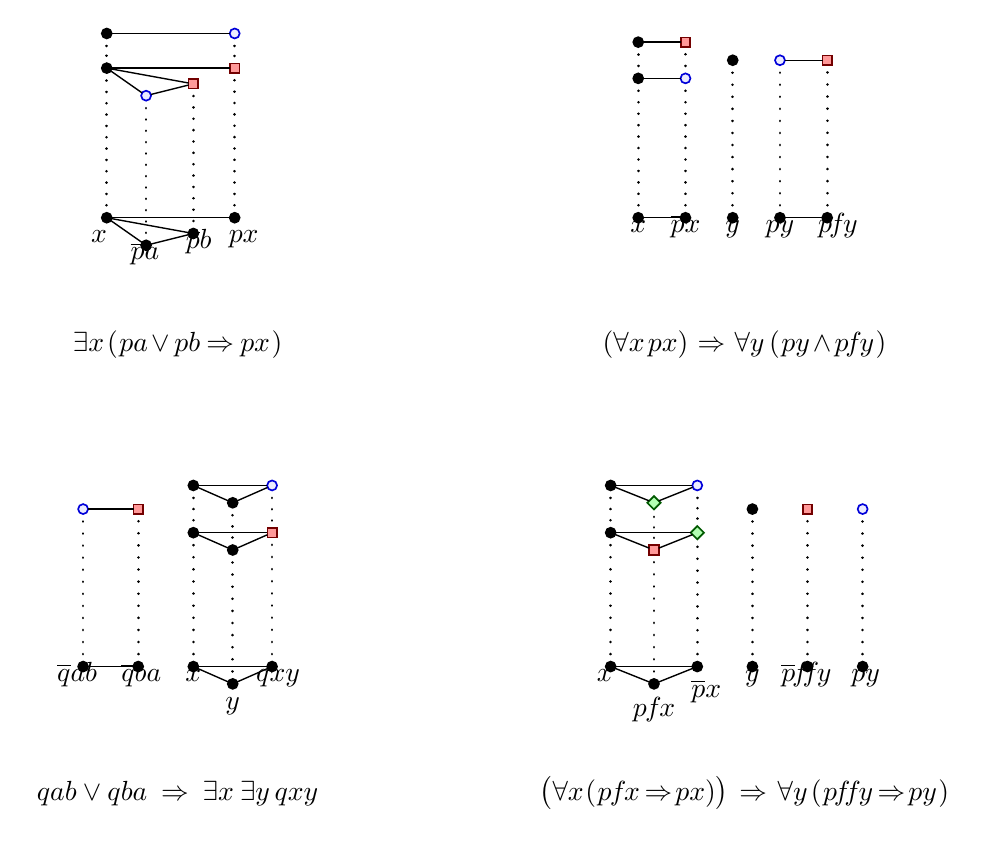
\begin{tikzpicture}\newcommand\radius{3.6}%
\begin{scope}[shift={(-\radius,5.7)}]{\cponeonformula}\end{scope}
\begin{scope}[shift={(\radius,5.7)}]{\cptwoonformula}\end{scope}
\begin{scope}[shift={(-\radius,0)}]{\cpthreeonformula}\end{scope}
\begin{scope}[shift={(\radius,0)}]{\cpfouronformula}\end{scope}
\end{tikzpicture}\end{center}%
\caption{\label{fig:cps}%
  Four combinatorial proofs, each shown above the formula proved.
  Here $x$ and $y$ are variables, $f$ is a unary function symbol, $a$ and $b$ are constants (nullary function symbols), $p$ is a unary predicate symbol, and $q$ is a binary predicate symbol.}\figrule\end{figure*}}






%%%%%%%%%% FIGURE Condensed forms of the four combinatorial proofs

\newcommand\eabcpinline{\fibration{
  \def\hi{.39}
  \def\vi{.66}
  \fibre{exbase}{\existsx}{
    \over{black vx}{\lo}{x}
    \over{black vx}{\hi}{xm}
    \over{black vx}{\vi}{xu}
  }
  \symb{\mkern2mu(\mkern2mu}
  \fibre{pabase}{\pa}{
    \over{blue vx}{\lo}{pa}
  }
  \symb{\tightvee\mkern1.2mu}
  \fibre{pybase}{\pb}{
    \over{red vx}{\lo}{pb}
  }
  \symb{\mkern-1mu\implies\mkern-1mu}
  \fibre{pxbase}{\px}{
    \over{red vx}{\lo}{px}
    \over{blue vx}{\hi}{pxm}
  }
  \symb{\mkern2mu)}
  \e {x}{pa}
  \e {pa}{pb}
  \draw (x) to[out=20,in=165,looseness=.85] (pb);
  \draw (xm) to[out=20,in=163,looseness=.8] (px);
  \draw (xu) to[out=20,in=163,looseness=.8] (pxm);
}}

\newcommand\pfycpinline{\fibration{
  \symb{(}
  \fibre{axbase}{\allx}{
     \over{black vx}{\lo}{xl}
     \over{black vx}{\hi}{xu}
  }
  \symb{\mkern2mu}
  \fibre{pxbase}{\px}{
    \over{blue vx}{\lo}{pxl}
    \over{red vx}{\hi}{pxu}
  }
  \symb{\mkern2mu)\mkern4mu\implies\mkern4mu}
  \fibre{aybase}{\ally}{
    \over{black vx}{\lo}{y}
  }
  \symb{\mkern2mu(\mkern1mu}
  \fibre{pybase}{\py}{
    \over{blue vx}{\lo}{py}
  }
  \symb{\mkern-2mu\wedge\mkern-2mu}
  \fibre{pfybase}{\pfy}{
    \over{red vx}{\lo}{pfy}
  }
  \symb{\mkern1mu)}
  \draw (xu) -- (pxu);
  \draw (xl) -- (pxl);
  \draw (py) -- (pfy);
}}


\newcommand\cponeinline{\eabcpinline}
\newcommand\cptwoinline{\pfycpinline}
\newcommand\cpthreeinline{\pabcpinline}
\newcommand\cpfourinline{\onioncpinline}



\newcommand\figcpscondensed{\begin{figure*}\begin{center}\vspace{-1ex}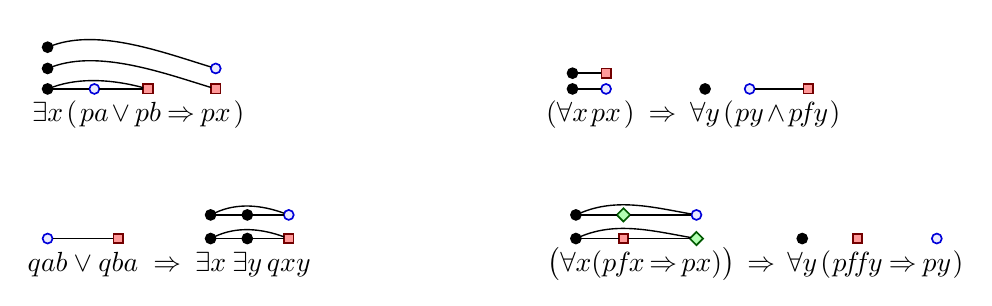
\begin{tikzpicture}\newcommand\radius{3.2}%
  \begin{scope}[shift={(-\radius,1.9)}]\cponeinline\end{scope}
  \begin{scope}[shift={(\radius,1.9)}]\cptwoinline\end{scope}
  \begin{scope}[shift={(-\radius,0)}]\cpthreeinline\end{scope}
  \begin{scope}[shift={(\radius,0)}]\cpfourinline\end{scope}
\end{tikzpicture}\end{center}%
\caption{\label{fig:cps-condensed}Condensed forms of the four combinatorial proofs in Fig.\,\ref{fig:cps}.}\figrule\vspace{-4ex}\end{figure*}}




%%%%%%% PICTURE: Drinker graph, cotree, binding graph


\newcommand\drinkersquare{
\lvx{-\halfedgelen,\halfedgelen}{x}{x}{135}
\lvx{\halfedgelen,\halfedgelen}{px}{\mkern.5mu\likex\ppx}{45}
\lvx{-\halfedgelen,-\halfedgelen}{y}{\mkern.5mu\likex y}{-135}
\lvx{\halfedgelen,-\halfedgelen}{py}{\py}{-45}
}
\newcommand\drinkersquareedges{
  \e x y
  \e x {px}
  \e x {py}
}

\newcommand\drinkersquarewithedges{\drinkersquare\drinkersquareedges}


\newcommand\drinkergraphpic{\gr{\drinkersquarewithedges}}

\newcommand\drinkercotreepic{\tr{\tikzset{level 1/.style={sibling distance=8ex},level 2/.style={sibling distance=4ex}}
  \joinroot
    child { \leaflab x }
    child { 
      \unionnode
      child { \leaflab y }
      child { \leaflab \ppx }
      child { \leaflab \py }
    }
  ;
}}

\newcommand\drinkerbindinggraphpic{\gr{\drinkersquare \de x {px} \de y {py}}}


%%%%%% PICTURE lifting diagrams

\newcommand\liftingdiagrams{%
\begin{center}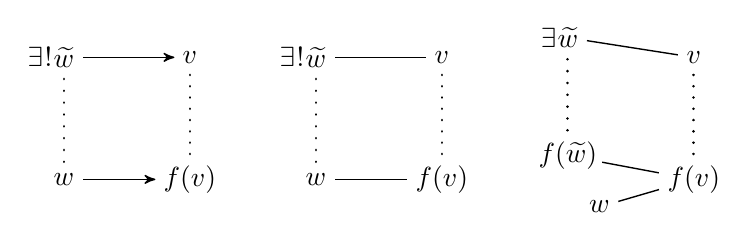
\begin{tikzpicture}[graph,outer sep=1.5pt,inner sep=0pt]\begin{math}
  \newcommand\rad{.8}
  \newcommand\vht{1.55}
  \newcommand\shortrad{.4}
  \newcommand\commonsquarepart{
    \node (liftw) at (-\rad,\vht) {$\skewlifting\vertexa$};
    \node[left=-1pt of liftw,outer sep=0,inner sep=0] (uniqueliftw) {$\exists\mkern1mu!$};
    \node (w) at (-\rad,0) {$\vertexa$};
    \node (v) at (\rad,1.55) {$v$};
    \node (fv) at (\rad,0) {$\fib(v)$};
    % fibres
    \begin{scope}[fibres]
      \fe{liftw}{w}
      \fe{v}{fv}
    \end{scope}
  }
  \begin{scope}[shift={(-3.2,0)}]    
    \commonsquarepart
    % directed edges
    \deseps {w} {fv} {1.8pt} {1.5pt}
    \deseps {liftw} {v} {1.8pt} {1.5pt}
  \end{scope}
  \begin{scope}
    \commonsquarepart
    % undirected edges
    \eseps {w} {fv} {1.7pt} {1.7pt}
    \eseps {liftw} {v} {1.7pt} {1.7pt}
  \end{scope}
  \begin{scope}[shift={(3.2,0)}]    
    \node (v) at (\rad,1.55) {$v$};
    \node (fv) at (\rad,0) {$f(v)$};
    \node (fliftw) at (-\rad,.3){$f(\skewlifting w)$};
    \node (liftw) at (-\rad,1.8){$\skewlifting\vertexa$};
    \node[left=-1pt of liftw,outer sep=0,inner sep=0] (uniqueliftw) {$\exists$};
    \node (w) at (-\shortrad,-.35) {$w$};
    % undirected edges
    \eseps {w} {fv} {1.7pt} {1.7pt}
    \eseps {liftw} {v} {1.7pt} {1.7pt}
    \eseps {fliftw} {fv} {.3pt} {1.7pt}
  \end{scope}
  \begin{scope}[fibres]
    \fe{liftw}{fliftw}
    \fe{v}{fv}
  \end{scope}
\end{math}\end{tikzpicture}\end{center}}




%%%%%%% FIGURE: Drinker bifibration, binding fibration, and skeleton

% add a label to a vertex
% relative positioning using polar coordinates https://www.latex4technics.com/?note=30vp
\tikzset{
    position/.style args={#1:#2 from #3}{
        at=(#3.#1), anchor=#1+180, shift=(#1:#2)
    }
}
\newcommand\labsep[4]{% #1 point-being-labelled, #2 contents, #3 angle, #4 labelsep
%\node (label) at ([shift={(#1)}] #3:#4) {\ensuremath{#2}};}
\node[outer sep=0,inner sep=0,position=#3:#4 from #1] {\ensuremath{#2}};}

\newcommand\coverylabelangle{-35}
\newcommand\coverppxlabelangle{0}
\newcommand\coverppxlabeldist{2pt}
\newcommand\addalldrinkercoverlabels[3]{% #1 = upper x variant, #2 = lower x variant, #3 = universal binder var
  \labsep{xa}{#1}{170}{2pt}
  \labsep{xb}{#2}{-170}{2pt}
  \labsep{ya}{\likex #3}{\coverylabelangle}{2pt}
  \labsep{ppxb}{\likex{\mkern-1mu\pp\mkern-.6mu #2}}{\coverppxlabelangle}{\coverppxlabeldist}
  \labsep{pya}{\likex{p #3}}{0}{2pt}
}
\newcommand\adddrinkercoverlabels[2]{\addalldrinkercoverlabels{#1}{#2}{y}}

\newcommand\drinkercoververtices{
  \begin{scope}[shift={(0,\drinkercovergap)}]
    \vx{\drinkerx,0}{xa}
    \vx{\drinkerxxx,-\drinkercoverseconddown}{ya}
    \vx{\drinkerxxxx,0}{pya}
  \end{scope}
  \vx{\drinkerx,0}{xb}
  \vx{\drinkerxx,-\drinkercoverfirstdown}{ppxb}
}

\newcommand\drinkercover{
  \drinkercoververtices
  \drinkercoveredges
}

\newcommand\drinkerfib{
\begin{scope}[shift={(0,\fibheight)}]
  \drinkercover
\end{scope}
\drinkerbase
\drinkerfibres
}

\newcommand\drinkerfiblabelledpair[2]{% #1 = upper x variant, #2 = lower x variant
  \drinkerfib
  \adddrinkercoverlabels{#1}{#2}
}

\newcommand\drinkerfibvertices{
  \drinkerbasevertices
  \begin{scope}[shift={(0,\fibheight)}]\drinkercoververtices\end{scope}
}

\newcommand\drinkerfibverticesandfibres{
  \drinkerfibvertices
  \drinkerfibres
}

\newcommand\drinkerbindingfiblabelled[2]{% #1 = upper x variant, #2 = lower x variant
  \drinkerfibverticesandfibres
  \adddrinkercoverlabels{#1}{#2}
  \de{ya}{pya}
  \de{xb}{ppxb}
  \de{y}{py}
  \de{x}{ppx}
}


\newcommand\figdrinkerbifib{\begin{figure*}%
\begin{center}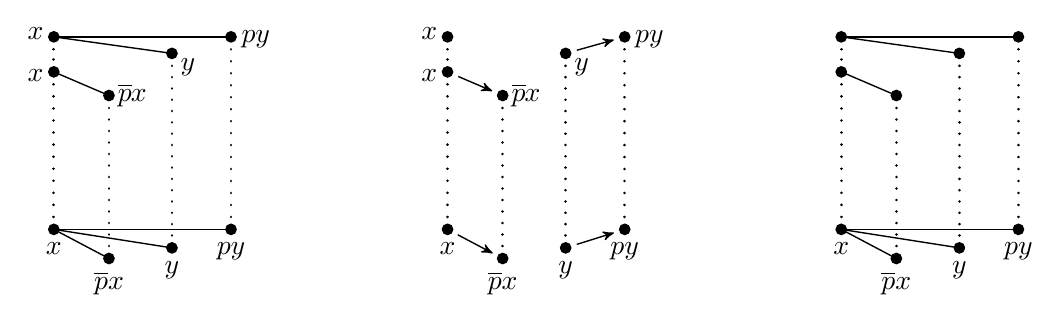
\begin{tikzpicture}[graph]
  \begin{scope}[shift={(-5,0)}]\drinkerfiblabelledpair{x}{x}\end{scope}
  \begin{scope}[shift={(0,0)}]\drinkerbindingfiblabelled{x}{x}\end{scope}
  \begin{scope}[shift={(5,0)}]\drinkerfib\end{scope}
\end{tikzpicture}\end{center}\caption{\label{fig:drinkerbifib}A skew bifibration (left), its binding fibration (centre), and its skeleton (right).}\figrule\end{figure*}}








\begin{document}
\vlnosmallleftlabels%
\bstctlcite{refs:BSTcontrol}%
%
% paper title
% Titles are generally capitalized except for words such as a, an, and, as,
% at, but, by, for, in, nor, of, on, or, the, to and up, which are usually
% not capitalized unless they are the first or last word of the title.
% Linebreaks \\ can be used within to get better formatting as desired.
% Do not put math or special symbols in the title.
\title{Combinatorial Proofs and Decomposition Theorems for First-order Logic\vspace{-3ex}}


% author names and affiliations
% use a multiple column layout for up to three different
% affiliations

%% \author{\IEEEauthorblockN{Dominic J. D. Hughes}
%% \IEEEauthorblockA{}
%% \and
%% \IEEEauthorblockN{Lutz Straßburger}
%% \IEEEauthorblockA{Inria, Equipe Partout\\
%% Ecole Polytechnique, LIX \\ %UMR 7161\\
%% France}
%% \and
%% \IEEEauthorblockN{Jui-Hsuan Wu}
%% \IEEEauthorblockA{Ecole Normale Supérieure\\
%% France}}

% conference papers do not typically use \thanks and this command
% is locked out in conference mode. If really needed, such as for
% the acknowledgment of grants, issue a \IEEEoverridecommandlockouts
% after \documentclass

% for over three affiliations, or if they all won't fit within the width
% of the page, use this alternative format:
% 
%\author{\IEEEauthorblockN{Michael Shell\IEEEauthorrefmark{1},
%Homer Simpson\IEEEauthorrefmark{2},
%James Kirk\IEEEauthorrefmark{3}, 
%Montgomery Scott\IEEEauthorrefmark{3} and
%Eldon Tyrell\IEEEauthorrefmark{4}}
%\IEEEauthorblockA{\IEEEauthorrefmark{1}School of Electrical and Computer Engineering\\
%Georgia Institute of Technology,
%Atlanta, Georgia 30332--0250\\ Email: see http://www.michaelshell.org/contact.html}
%\IEEEauthorblockA{\IEEEauthorrefmark{2}Twentieth Century Fox, Springfield, USA\\
%Email: homer@thesimpsons.com}
%\IEEEauthorblockA{\IEEEauthorrefmark{3}Starfleet Academy, San Francisco, California 96678-2391\\
%Telephone: (800) 555--1212, Fax: (888) 555--1212}
%\IEEEauthorblockA{\IEEEauthorrefmark{4}Tyrell Inc., 123 Replicant Street, Los Angeles, California 90210--4321}}




% use for special paper notices
%\IEEEspecialpapernotice{(Invited Paper)}




% make the title area
\maketitle

% As a general rule, do not put math, special symbols or citations
% in the abstract
\begin{abstract}
  We uncover a close relationship between combinatorial and
  syntactic proofs for first-order logic. Whereas syntactic proofs are
  formalized in a deductive proof system based on inference rules,
  a combinatorial proof is a syntax-fre presentation of a proof
  that is independent from any set of inference rules. We show that
  the two proof representations are related via a deep inference
  decomposition theorem that establishes a new kind of normal form
  for syntactic proofs. This yields (a) a simple proof
  of soundness and completeness for first-order combinatorial
  proofs, and (b) a full completeness theorem: every combinatorial
  proof is the image of a syntactic proof.
\end{abstract}

% no keywords




% For peer review papers, you can put extra information on the cover
% page as needed:
% \ifCLASSOPTIONpeerreview
% \begin{center} \bfseries EDICS Category: 3-BBND \end{center}
% \fi
%
% For peerreview papers, this IEEEtran command inserts a page break and
% creates the second title. It will be ignored for other modes.
\IEEEpeerreviewmaketitle

\linenumbers

%%%%%%%%%%%%%%%%%%%%%%%%%%%%%%%%%%%%%%%%%%%%%%%%%%%%%%%%%%%%%%%%%%%%%%%%%%
%%%%%%%%%%%%%%%%%%%%%%%%%%%%%%%%%%%%%%%%%%%%%%%%%%%%%%%%%%%%%%%%%%%%%%%%%%
%%%%%%%%%%%%%%%%%%%%%%%%%%%%%%%%%%%%%%%%%%%%%%%%%%%%%%%%%%%%%%%%%%%%%%%%%%
%%%%%%%%%%%%%%%%%%%%%%%%%%%%%%%%%%%%%%%%%%%%%%%%%%%%%%%%%%%%%%%%%%%%%%%%%%

%\todo{Examples,examples,examples}
\section{Introduction}

First-order predicate logic is a cornerstone of modern
logic. Since its formalisation by Frege~\cite{frege:79} it has seen a
growing usage in many fields of mathematics and computer science. Upon
the development of proof theory by Hilbert~\cite{hilbert:22},
\emph{proofs} became first-class citizens as mathematical objects that
could be studied on their own. Since Gentzen's \emph{sequent
calculus}~\cite{gentzen:35:I,gentzen:35:II}, many other proof systems
have been developed that allow the implementation of efficient proof
search, for example \emph{analytic tableaux}~\cite{smullyan:68} or
\emph{resolution}~\cite{robinson:65}. Despite the immense progress
made in proof theory in general and in the area of
automated and interactive theorem provers in
particular, we still have
no satisfactory notion of proof identity for first-order logic. In
this respect, proof theory is quite different from any other
mathematical field. For example in group theory, two groups are
\emph{the same} iff they are isomorphic; in topology, two spaces are
\emph{the same} iff they are homeomorphic; etc. In proof theory, we
have no such notion telling us when two proofs are \emph{the same},
even though Hilbert was considering this problem as a possible 24th
problem for his famous lecture~\cite{hilbert:00} in
1900~\cite{thiele:03}, before proof theory existed as a mathematical
field.

The main reason for this problem is that formal proofs, as they are
usually studied in logic, are inextricably tied to the syntactic
(inference rule based) proof system in which they are carried out. And
it is difficult to compare two proofs that are produced within two
different syntactic proof systems, based on different sets of inference rules.
%
\newcommand\lkpeirceproof{
\vlderivation{
  \vlin{\vlor}{}{\sqn{\peirceformula}}{
    \vlin{\conr}{}{\sqn{(\cneg{p} \vlor q) \vlan \cneg{p}, p}}{
      \vliin{\vlan}{}{\sqn{(\cneg{p} \vlor q) \vlan \cneg{p}, p, p}}{
        \vlin{\vlor}{}{\sqn{\cneg{p} \vlor q, p}}{
          \vlin{\weakr}{}{\sqn{\cneg{p}, q, p}}{
            \vlin{\axr}{}{\sqn{\cneg{p}, p}}{
              \vlhy{}}}}}{
        \vlin{\axr}{}{\sqn{\cneg{p}, p}}{
          \vlhy{}}}}}}
}
\newcommand\dipeirceproof{
\vlderivation{
  \vlin{\acD}{}{\peirceformula}{
    \vlin{\fequ}{}{((\cneg{p} \vlor q) \vlan \cneg{p}) \vlor (p \vlor p)}{
      \vlin{\sw}{}{(\cneg{p} \vlan (\cneg{p} \vlor q)) \vlor p) \vlor p}{
        \vlin{\fequ}{}{(\cneg{p} \vlan ((\cneg{p} \vlor q) \vlor p)) \vlor p)}{
          \vlin{\sw}{}{(p \vlor (\cneg{p} \vlor q)) \vlan \cneg{p}) \vlor p}{
            \vlin{\aiD}{}{(p \vlor (\cneg{p} \vlor q)) \vlan (\cneg{p} \vlor p)}{
              \vlin{\tttD}{}{(p \vlor (\cneg{p} \vlor q)) \vlan \ttt}{
                \vlin{\fequ}{}{p \vlor (\cneg{p} \vlor q)}{
                  \vlin{\wrD}{}{(p \vlor \cneg{p}) \vlor q}{
                    \vlin{\aiD}{}{p \vlor \cneg{p}}{
                      \vlhy{\ttt}}}}}}}}}}}}
}
\newcommand\lkdrinkerproof{
\vlderivation{
  \vlin{\conr}{}{\sqn{\exists x.(\cneg{p}x \vlor (\forall y.py))}}{
    \vlin{\exists}{}{\sqn{\exists x.(\cneg{p}x \vlor (\forall y.py)),\exists
x.(\cneg{p}x \vlor (\forall y.py))}}{
      \vlin{\vlor}{}{\sqn{\cneg{p}w \vlor (\forall y.py), \exists
x.(\cneg{p}x \vlor (\forall y.p(y)))}}{
        \vlin{\forall}{}{\sqn{\cneg{p}w, \forall y.py, \exists
x.(\cneg{p}x \vlor (\forall y.py))}}{
          \vlin{\exists}{}{\sqn{\cneg{p}w, pz, \exists
x.(\cneg{p}x \vlor (\forall y.py))}}{
            \vlin{\vlor}{}{\sqn{\cneg{p}w, pz, \cneg{p}z \vlor (\forall y.py))}}{
              \vlin{\weakr}{}{\sqn{\cneg{p}w, pz, \cneg{p}z, (\forall y.py))}}{
                \vlin{\weakr}{}{\sqn{\cneg{p}w, pz, \cneg{p}z}}{
                \vlin{\axr}{}{\sqn{pz, \cneg{p}z}}{
                  \vlhy{}}}}}}}}}}}
}
\newcommand\ksonedrinkerproof{
\vlderivation{
  \vlin{\acD}{}{\exists x.(\cneg{p}x \vlor (\forall y.py))}{
    \vlin{\mfaD}{}{\exists x.(\cneg{p}x \vlor (\forall y.(py \vlor py)))}{
      \vlin{\acD}{}{\exists x.(\cneg{p}x \vlor ((\forall y.py) \vlor (\forall y.py)))}{
        \vlin{\fequ}{}{\exists x.((\cneg{p}x \vlor \cneg{p}x) \vlor ((\forall y.py) \vlor (\forall y.py)))}{
          \vlin{\mexD}{}{\exists x.((\cneg{p}x \vlor (\forall y.py)) \vlor (\cneg{p}x \vlor (\forall y.py)))}{
            \vlin{\exists}{}{(\exists x.(\cneg{p}x \vlor (\forall y.py))) \vlor (\exists x.(\cneg{p}x \vlor (\forall y.py)))}{
              \vlin{\fequ}{}{(\cneg{p}w \vlor (\forall y.py)) \vlor (\exists x.(\cneg{p}x \vlor (\forall y.py)))}{
                \vlin{\exists}{}{\forall y.((\cneg{p}w \vlor py) \vlor (\exists x.(\cneg{p}x \vlor (\forall y.py))))}{
                  \vlin{\fequ}{}{\forall y.((\cneg{p}w \vlor py) \vlor (\cneg{p}y \vlor (\forall y.py)))}{
                    \vlin{\wD}{}{\forall y.((py \vlor \cneg{p}y) \vlor (\cneg{p}w \vlor (\forall y.py)))}{
                      \vlin{\aiD}{}{\forall y.(py \vlor \cneg{p}y)}{
                        \vlin{\forall}{}{\forall y.\ttt}{
                          \vlhy{\ttt}}}}}}}}}}}}}}
}
\begin{figure}\vspace{-2ex}\begin{center}\hspace*{-0ex}\begin{math}
\newcommand\peircescale{.75}
\newcommand\drinkerscale{\peircescale}
\newcommand\cpscale{.9}
\begin{array}{@{}c@{\hspace{4ex}}c@{}}
{}\scalebox{\peircescale}{$\lkpeirceproof$}
&
{}\scalebox{\drinkerscale}{$\lkdrinkerproof$}
\\[13ex]
\downarrow
&
\downarrow
\\[1ex]
\vctr{\scalebox{\cpscale}{\peircecppic}}
&
\vctr{\raisebox{-2ex}[16.5ex]{\scalebox{\cpscale}{\drinkerfibcolouredpic}}}
\\[10ex]
\uparrow
&
\uparrow
\\[2ex]
{}\scalebox{\peircescale}{$\dipeirceproof$}
&
{}\scalebox{\drinkerscale}{$\ksonedrinkerproof$}
%
\end{array}
\end{math}\hspace*{-8ex}\end{center}\caption{Left:
syntactic proofs in sequent calculus (above)
and the calculus of structures (below)
which translate to the same propositional combinatorial proof (centre).
%
Right:
syntactic proofs 
in sequent calculus (above)
and the new calculus $\FOKS$ introduced in this paper (below),
which translate to the same first-order combinatorial proof (centre).%
% two syntactic proofs of 
% $\protect\peirceformula$,
% in the sequent calculus (above)
% and in the calculus of structures (below),
% which translate to the same propositional combinatorial proof (centre).
% %
% Right:
% two syntactic proofs of 
% $\protect\veedrinkerformula$,
% in the sequent calculus (above)
% and the new calculus $\FOKS$ introduced in this paper (below),
% which translate to the same first-order combinatorial proof (centre).%
}\label{fig:translate}\vspace{-4ex}\end{figure}%

This is where \emph{combinatorial proofs} come in. They were
introduced by Hughes~\cite{hughes:pws} for classical propositional
logic as a syntax-free notion of proof, and as a potential solution
to Hilbert's 24th problem~\cite{hughes:invar} (see
also~\cite{str:hilbert:24}). The basic idea is to abstract away from
the syntax of the inference rules used in inductively-generated proofs
and consider the proof as a combinatorial object, more precisely
as a special kind of
graph homomorphism. For example, a propositional combinatorial
proof of Peirce's law $\peirceimpliesformula=\peirceformula$ is shown mid-left in
Fig.\,\ref{fig:translate},
%depicted below-left,
a homomorphism from a coloured graph to a graph labelled with
propositional variables.
%
% \begin{center}\vspace{.5ex}\begin{tikzpicture}\newcommand\radius{2.3}
%   \begin{scope}[shift={(-\radius,0)}]{\peircecp}\end{scope}
%   \begin{scope}[shift={(\radius,0)}]{\drinkerfibcoloured}\end{scope}
% \end{tikzpicture}\vspace{0ex}\end{center}
% %
% 
% \begin{equation*}
%   \scalebox{.7}{$\lkdrinkerproof
% %\qquad
% \ksonedrinkerproof
% $}
% \end{equation*}
% 
% \juihsuan{LK1 and KS1 proofs of Peirce's law and LK1 proof of drinker formula}
% \lutz{can you also do the KS1 for the drinker?}
% \juihsuan{done}

Several authors have illustrated how syntactic proofs in various
proof systems can be translated to propositional combinatorial proofs:
for sequent proofs in~\cite{hughes:invar}, for deep inference proofs
in~\cite{str:fscd17}, for Frege systems in~\cite{str:RR-9048}, and for
tableaux systems and resolution in~\cite{acc:str:18}. This enables a
natural definition of proof identity for propositional logic: two
proofs are \emph{the same}, if they are mapped to the same
combinatorial proof.
%
For example, the left side of Fig.\,\ref{fig:translate} translates
syntactic proofs from sequent calculus and the calculus of structures into
the same combinatorial proofs, witnessing that the two syntactic proofs,
from different systems, are \emph{the same}.

Recently, Acclavio and Stra\ss burger extended this notion to relevant
logics~\cite{acc:str:relevant} and to modal
logics~\cite{acc:str:modal}, and Heijlties, Hughes and Stra\ss burger
have provided combinatorial proofs for intuitionistic propositional
logic~\cite{HHS:lics19}.

In this paper we advance the idea that combinatorial proofs can provide
a notion of proof identity for first-order logic. \emph{First-order
combinatorial proofs} were introduced by Hughes in~\cite{hughes:fopws}.
For example, a first-order combinatorial proof of Smullyan's 
``drinker paradox'' $\drinkerformula=\veedrinkerformula$ is shown on the
right of Fig.\,\ref{fig:translate},\todo{wrong implies symbol in drinkerformula?}
a homomorphism from a partially coloured graph to a labelled graph.
However, even though Hughes proves soundness and completeness, the 
proof is highly unsatisfactory: (1) the soundness argument is extremely
long, intricate and cumbersome, and (2) the completeness proof does not 
allow a syntactic proof to be read back from a combinatorial proof, i.e.,
completeness is not
\emph{sequentializable} \cite{girard:87} or
\emph{full}~\cite{abramsky:jagadeesan:94}.\dominic{ok to say sequentializable too?}
%
A fundamental problem is that not all combinatorial
proofs can be obtained as translations of sequent calculus proofs.

We solve these issues by moving to a deep inference
system. More precisely, we introduce a new proof system, called
$\FOKS$, for first-order logic, that (a) reflects every combinatorial
proof, i.e., there is a surjection from $\FOKS$ proofs to
combinatorial proofs, (b) yields far simpler proofs of
soundness and completeness for combinatorial proofs, and (c) admits
new decomposition theorems establishing a precise correspondence
between certain syntactic inference rules and certain combinatorial
notions.
%
The right side of Fig.\,\ref{fig:translate}
illustrates the surjection in (a), and since the syntactic proofs 
of the two systems both translate the same combinatorial proof,
they can be considered \emph{the same}.

In general, a \emph{decomposition theorem} provides normal forms of
proofs, separating subsets of inference rules of a proof system. A
prominent example of a decomposition theorem is Herbrand's
theorem~\cite{herbrand:phd}, which allows a separation between the
propositional part and the quantifier part in a first-order
proof~\cite{gentzen:35:II,brunnler:06:herbrand}. Through the advent of
deep inference, new kinds of proof decompositions became possible,
most notably the separation between the linear part of a proof and the
resource management of a proof. It has been shown by
Stra{\ss}burger~\cite{str:07:RTA} that a proof in classical
propositional logic can be decomposed into a proof of multiplicative
linear logic, followed by a proof consisting only of contractions and
weakenings. In this paper we show that the same is possible for
first-order logic.

Combinatorial proofs and deep inference can be seen as opposite ends
of a spectrum: whereas deep inference allows for a very fine
granularity of inference rules---one inference rule in a standard
formalism, like sequent calculus or semantic tableaux, is usually
simulated by a sequence of different deep inference rules---
combinatorial proofs have completely abolished the concept of inference
rule. And yet, there is a close relationship between the two,
realized through a decomposition theorem, as we establish in this
paper.



% \subsection{Pictures that could be used elsewhere in the paper}
% 
% 
% Condensed combinatorial proof of drinker formula(s):
% %
% \begin{center}\vspace{3ex}\begin{math}
% \begin{tikzpicture}
% \drinkerInline
% \end{tikzpicture}
% \hspace{10ex}
% \begin{tikzpicture}
% \veedrinkerInline
% \end{tikzpicture}\end{math}\end{center}


%%\figcps Fig.\,\ref{fig:cps} is a floating figure with four combinatorial proofs.

%%\figcpscondensed Fig.\,\ref{fig:cps-condensed} is a floating figure with the condensed forms of the four combinatorial proofs in Fig.\,\ref{fig:cps}.



% Illustrating why we need to collapse twins during contraction, to preserve the target as a fograph:
% %
% \twincollapsepic
% %
% Aligning both $\singleton{}\mkern4mu\singleton[red]{}$ and
% $\singleton{}\mkern4mu\singleton[blue]{}$ over
% a single copy of $\forall y\mkern2mu\py$
% results in two uncoloured vertices
% \raisebox{2pt}[0ex][0ex]{$\column{\singleton{}\\[-1.6ex]\singleton{}}$\hspace{-2pt}}
% over $\forall y$.
% %
% The cover therefore fails to be a fograph: both uncoloured vertices are implicitly labelled with $y$ and
% so are outer $y$-binders in the scope of each other.
% %
% The correct operation is shown above-right,
% in which the troublesome pair is collapsed to a single uncoloured vertex $\singleton{}$ over $\forall y$.


%%%%%%%%%%%%%%%%%%%%%%%%%%%%%%%%%%%%%%%%%%%%%%%%%%%%%%%%%%%%%%%%%%%%%%%%%%
%%%%%%%%%%%%%%%%%%%%%%%%%%%%%%%%%%%%%%%%%%%%%%%%%%%%%%%%%%%%%%%%%%%%%%%%%%
%%%%%%%%%%%%%%%%%%%%%%%%%%%%%%%%%%%%%%%%%%%%%%%%%%%%%%%%%%%%%%%%%%%%%%%%%%
%%%%%%%%%%%%%%%%%%%%%%%%%%%%%%%%%%%%%%%%%%%%%%%%%%%%%%%%%%%%%%%%%%%%%%%%%%

\section{Preliminaries: First-order Logic}\label{sec:fologic}

\subsection{Terms and Formulas}

Fix pairwise disjoint countable sets $\VAR=\set{x,y,z,\ldots}$ of variables,
$\FUN=\set{f,g,\ldots}$ of function symbols, and 
$\PRED=\set{p,q,\ldots}$ of predicate symbols. Each function symbol and
each predicate symbol has a finite arity. The grammars below generate
the set $\TERM$ of \bfit{terms}, denoted by $s,t,u,\ldots$, the set
$\ATOM$ of \bfit{atoms}, denoted by $a,b,c,\ldots$, and the set
$\FORM$ of \bfit{formulas}, denoted by $A,B,C,\ldots$:
\begin{equation*}
  \begin{array}{r@{~}l}
    t &\coloneqq~ x \mid f(t_1,\dots,t_n)
    \\[.5ex]
    a &\coloneqq~ \ttt\mid\fff\mid p(t_1,\dots,t_n) \mid \dual p(t_1,\dots,t_n)
    \\[.5ex]
    A &\coloneqq~ a \mid A\vlan A \mid A\vlor A \mid \exists x.A \mid \forall x.A
\end{array}
\end{equation*}
where the arity of $f$ and $p$ is $n$.
For better readability of often omit parentheses and write simply $ft_1 \dots t_n$ or $pt_1 \dots t_n$.
We consider the truth constants
$\ttt$ (\emph{true}) and $\fff$
(\emph{false}) as additional atoms, and we consider all formulas in negation
normal form, where \bfit{negation} $(\dual\cdot)$ is defined on
atoms and formulas via De Morgan's laws:
\begin{equation*}
  \begin{array}{ccc}
    \dual{\dual a} = a
    &
  \dual\ttt =\fff &
  \dual{p(t_1,\ldots,t_n)} = \dual{p}(t_1,\ldots,t_n) \\[.5ex]
  &
  \dual\fff = \ttt &
  \dual{\dual p(t_1,\ldots,t_n)} = p(t_1,\ldots,t_n) \\[.5ex]
  &
  \dual{\exists x.A} = \forall x.\dual{A}
  &
  \dual{A \vlan B} = \dual{A} \ \vlor \ \dual{B} 
  \\[.5ex]
  &
  \dual{\forall x.A} = \exists x.\dual{A}
  &
%  \\[.5ex]
  \dual{A \vlor B} = \dual{A} \ \vlan \ \dual{B}
  \end{array}
\end{equation*}
Then we write $A\implies B$ as abbreviation for $\dual A\vlor B$.

A formula is \bfit{rectified} if all bound variables are distinct from
one another and from all free variables. Every formula can be
transformed into a logically equivalent rectified form, by simply
renaming the bound variables. If we consider formulas equivalent
modulo $\alpha$-conversion (renaming of bound variables), then the
rectified form of a formula $A$ is uniquely defined, and we denote it
by $\rectif A$.


A \bfit{substitution} is a function $\sigma\colon\VAR\to\TERM$ that is
the identity almost everywhere. We denote substitutions as
$\sigma=\sublist{\subst{x_1}{t_1},\ldots,\subst{x_n}{t_n}}$, where
$\sigma(x_i)=t_i$ for $i=1..n$ and $\sigma(x)=x$ for all
$x\notin\set{x_1,\ldots,x_n}$. 
Write $A\sigma$ for the formula
obtained from $A$ by applying $\sigma$, i.e., by simultaneously
replacing all occurrences of $x_i$ by $t_i$.
A \bfit{variable renaming} is a substitution $\rho$ with $\rho(x)\in\VAR$ for all variables $x$.

%%%%%%%%%%%%%%%%%%%%%%%%%%%%%%%%%%%%%%%%%%%%%%%%%%%%%%%%%%%%%%%%%
%%%%%%%%%%%%%%%%%%%%%%%%%%%%%%%%%%%%%%%%%%%%%%%%%%%%%%%%%%%%%%%%%

\subsection{Sequent Calculus $\FOLK$}

\begin{figure}[!t]
  \begin{center}
    \framebox{%
      $
      \begin{array}{@{}c@{}}
        \dbox{%
          $
          \begin{array}{c}
            \vlinf{\axr}{}{\sqn{a,\cneg a}}{}
            \qquad
            \vlinf{\ttt}{}{\sqn{\ttt}}{}
            \qquad
            \vliinf{\mixr}{}{\sqn{\Gamma,\Delta}}{\sqn\Gamma}{\sqn\Delta}
            \\ \\[-1ex]
            \vlinf{\vlor}{}{\sqn{\Gamma,A\vlor B}}{\sqn{\Gamma,A,B}}
            \qquad
            \vliinf{\vlan}{}{\sqn{\Gamma,A\vlan B, \Delta}}{\sqn{\Gamma,A}}{\sqn{B,\Delta}}
            \\ \\[-1ex]
            \vlinf{\exists}{}{\sqn{\Gamma,\exists x.A}}{\sqn{\Gamma,A\ssubst{x}{t}}}
            \qquad
            \vlinf{\forall}{\text{($x$ not free in $\Gamma$)}}{\sqn{\Gamma,\forall x.A}}{\sqn{\Gamma,A}}
          \end{array}
          $%
        }%
        \\\\[-1ex]
        \vlinf{\conr}{}{\sqn{\Gamma,A}}{\sqn{\Gamma,A,A}}
        \qquad
        \vlinf{\weakr}{}{\sqn{\Gamma,A}}{\sqn{\Gamma}}
      \end{array}
      $
    }
  \end{center}
  \caption{Sequent calculi $\FOLK$ (all rules) and $\FOMLL$ (rules in the dashed box)}
  \label{fig:LK1}
\end{figure}

\bfit{Sequents}, denoted by $\Gamma,\Delta,\ldots$, are finite
multisets of formulas, written as lists, separated by comma. The
\bfit{corresponding formula} of a (non-empty) sequent $\Gamma=A_1,A_2,\ldots,A_n$
is the disjunction of its formulas: $\form\Gamma=A_1\vlor
A_2\vlor\cdots\vlor A_n$. A sequent is \bfit{rectified} iff its
corresponding formula is.\dominic{I changed fm$(\Gamma)$ to $\form\Gamma$,
easier for referee to understand/intuit/remember later in the paper}

In this paper we use the sequent calculus $\FOLK$, shown in
Figure~\ref{fig:LK1}, which is a one-sided variant of Gentzen's
original calculus~\cite{gentzen:35:I} for first-order logic. To
simplify some technicalities later in this paper, we include
the $\mixr$-rule.
%
\begin{thm}
  $\FOLK$ is sound and complete for first-order logic.
\end{thm}
%
\noindent For a proof, see any standard textbook, e.g.~\cite{TS:00}.

The linear fragment of $\FOLK$, i.e., the fragment
without the rules $\conr$ (\emph{contraction}) and $\weakr$
(\emph{weakening}) defines \emph{first-order multiplicative linear
logic}~\cite{girard:87,girard:88} \emph{with
mix}~\cite{fleury:retore:94,bellin:97}~(MLL1+mix). We denote that system
here with $\FOMLL$ (shown in Figure~\ref{fig:LK1} in the dashed box).

We will employ the cut elimination theorem. The \bfit{cut} rule is
\begin{equation}
  \vliinf{\cutr}{}{\sqn{\Gamma,\Delta}}{\sqn{\Gamma,A}}{\sqn{\dual A,\Delta}}
\end{equation}

\begin{thm}
  \label{thm:cutelim}
  If a sequent $\sqn\Gamma$ is provable in $\FOLKcut$ then it is also
  provable in $\FOLK$. Furthermore, if $\sqn\Gamma$ is provable in
  $\FOMLLcut$ then it is also provable in $\FOMLL$.
\end{thm}
%
\noindent As before, this is standard, see e.g.~\cite{TS:00} for a proof.

%%%%%%%%%%%%%%%%%%%%%%%%%%%%%%%%%%%%%%%%%%%%%%%%%%%%%%%%%%%%%%%%%%%%%%%%%%
%%%%%%%%%%%%%%%%%%%%%%%%%%%%%%%%%%%%%%%%%%%%%%%%%%%%%%%%%%%%%%%%%%%%%%%%%%
%%%%%%%%%%%%%%%%%%%%%%%%%%%%%%%%%%%%%%%%%%%%%%%%%%%%%%%%%%%%%%%%%%%%%%%%%%
%%%%%%%%%%%%%%%%%%%%%%%%%%%%%%%%%%%%%%%%%%%%%%%%%%%%%%%%%%%%%%%%%%%%%%%%%%


\section{Preliminaries: First-order Graphs}\label{sec:fographs}

\subsection{Graphs}

A \bfit{graph} $\gG=\tuple{\vG,\eG}$ is a pair where $\vG$ is a finite
set of \bfit{vertices} and $\eG$ is a finite set of \bfit{edges},
which are two-element subsets of $\vG$. We write $vw$ for an edge
$\set{v,w}$.

The \bfit{complement} of a graph $\gG=\tuple{\vG,\eG}$ is
the graph $\compl\gG=\tuple{\vG,\compl\eG}$ where $vw\in\compl\eG$ iff
$vw\notin\eG$. 

Let $\gG=\tuple{\vG,\eG}$ and $\gH=\tuple{\vH,\eH}$ be graphs such
that $\vG\cap\vH=\emptyset$. A \bfit{homomorphism}
$\phi\colon\gG\to\gH$ is a function $\phi\colon\vG\to\vH$ such that if
$vw\in\eG$ then $\phi(v)\phi(w)\in\eH$. The \bfit{union} $\gG +\gH$ is
the graph $\tuple{\vG \cup\vH,\eG\cup \eH}$ and the \bfit{join} $\gG
\times \gH$ is the graph $\tuple{\vG \cup\vH,\eG \cup \eH \cup \set{vw
\mid v \in \vG, w \in \vH}}$.  A graph $\gG$ is \bfit{disconnected}
if $\gG=\gG_1+\gG_2$ for two non-empty graphs $\gG_1,\gG_2$, otherwise
it is \bfit{connected}. It is \bfit{coconnected} if its complement is
connected.

A graph $\gG$ is \bfit{labelled} in a set $L$ if each vertex $v\in\vG$
has an element $\labelof v\in L$ associated with it, its \bfit{label}.  A
graph $\gG$ is (partially) \bfit{coloured} if it carries a partial
equivalence relation $\linkingof\gG$ on $\vG$; each equivalence class is a
\bfit{colour}.  A \bfit{vertex renaming} of $\gG=\tuple{\vG,\eG}$
along a bijection $(\hat\cdot)\colon\vG\to\hat\vG$ is the graph
$\hat\gG=\tuple{\hat\vG,\set{\hat v\hat w\mid vw\in\eG}}$, with
colouring and/or labelling inherited (i.e., $\hat v\samecol\hat w$ if
$v\samecol w$, and $\ell(\hat v)=\ell(v)$). Following standard graph
theory, we identify graphs modulo vertex renaming.

A \bfit{directed graph} $\gG =\tuple{\vG,\eG}$ is a set $\vG$ of
\bfit{vertices} and a set $\eG\subseteq \vG\times\vG$ of \bfit{direct edges}.
A \bfit{directed graph homomorphism}
$\phi\colon\tuple{\vG,\eG}\to\tuple{\vH,\eH}$ is a function $\phi\colon\vG\to\vH$ such that if
$\pair{v,w}\in\eG$ then $\pair{\phi(v),\phi(w)}\in\eH$.


%%%%%%%%%%%%%%%%%%%%%%%%%%%%%%%%%%%%%%%%%%%%%%%%%%%%%%%%%%%%%%
%%%%%%%%%%%%%%%%%%%%%%%%%%%%%%%%%%%%%%%%%%%%%%%%%%%%%%%%%%%%%%

\subsection{Cographs}

A graph $\gH=\tuple{\vH,\eH}$ is a \bfit{subgraph} of a graph
$\gG=\tuple{\vG,\eG}$ if $\vH\subseteq\vG$ and $\eH\subseteq\eG$. It
is \bfit{induced} if $v,w\in\vH$ and $vw\in\eG$ implies $vw\in\eH$. An induced
subgraph of $\gG=\tuple{\vG,\eG}$ is uniquely determined by its set of vertices
$V$ and we denote it by $\gG[V]$.
A graph is \bfit{$\gH$-free} if it does not contain $\gH$ as an induced
subgraph.  The graph $\Pfour$ is the (undirected) graph
$\tuple{\set{v_1, v_2, v_3, v_4},\set{v_1v_2, v_2v_3, v_3v_4}}$.  A
\bfit{cograph} is a $P_4$-free undirected graph. The interest in
cographs for our paper comes from the following well-known fact.

\begin{thm}[\cite{duffin:65}]\label{thm:cograph}
  A graph is a cograph iff it can be constructed from the singletons
  via the operations $+$ and~$\times$.
\end{thm}

In a graph $\gG$, the \bfit{neighbourhood} $N(v)$ of a vertex $v \in\vG$ is defined as
the set $\set{w \mid vw \in\eG}$. A \bfit{module} is a set $M \subseteq \vG$
such that $N(v) \setminus M = N(w) \setminus M$
for all $v, w \in M$. A module $M$ is \bfit{strong} if for every
module $M'$, we have $M' \subseteq M$, $M \subseteq$ or $M \cap M' =
\emptyset$. A module is \bfit{proper} if it has two or more vertices.

%% Modules in cographs correspond precisely to the subtrees of the
%% cotrees (the term-trees constructing the graph via $+$ and~$\times$).\todo{Cotree
%% must alternate $+$ and $\times$. Skip this comment completely?}

%%%%%%%%%%%%%%%%%%%%%%%%%%%%%%%%%%%%%%%%%%%%%%%%%%%%%%%%%%%%%%
%%%%%%%%%%%%%%%%%%%%%%%%%%%%%%%%%%%%%%%%%%%%%%%%%%%%%%%%%%%%%%



\subsection{Fographs}

A cograph is \bfit{logical} if every vertex is labelled by either an
atom or variable, and it has at least one atom-labelled vertex. We
write $\single\alpha$ for an $\alpha$-labelled vertex. An
atom-labelled vertex is called a \bfit{literal} and a
variable-labelled vertex is called a \bfit{binder}. A binder labelled
with $x$ is called an \bfit{$x$-binder}. The \bfit{scope} of a binder
$b$ is the smallest proper strong module containing $b$.
An \bfit{$x$-literal} is a literal whose
atom contains the variable $x$. An $x$-binder \bfit{binds} every
$x$-literal in its scope.  In a logical cograph $\gG$, a binder $b$ is
\bfit{existential} (resp. \bfit{universal}) if, for every other vertex
$v$ in its scope, we have $bv \in \eG$ (resp. $bv \notin \eG$). An
$x$-binder is \bfit{legal} if its scope contains no other $x$-binder
and at least one literal.
%
\begin{definition}
A \bfit{first-order graph} or \bfit{fograph} is a logical cograph with legal binders. The
\bfit{binding graph} of a fograph $\gG$ is the directed graph $\bG=\tuple{\vG,
\set{(b, l) \mid b \text{ binds } l}}$.
\end{definition}
%
\noindent We define a mapping $\graphof\cdot$ from formulas to (labelled)
graphs, inductively as follows:
%% For a formula $A$, we can define its
%% associated fograph $\graphof{A}$ inductively by:\todo{duplicate two sentences above}
\begin{equation*}
  \begin{array}{r@{\;}l@{\hskip4em}r@{\;}l}
    \graphof{a} &= \single a \rlap{\hskip1em(for any atom $a$)}  \\[.9ex]
    \graphof{A \cor B} &= \graphof{A} + \graphof{B} &
    \graphof{\exists x . A} &= \single x \times \graphof{A} \\[.9ex]
    \graphof{A \cand B} &= \graphof{A} \times \graphof{B} &
    \graphof{\forall x . A} &= \single x + \graphof{A}    
  \end{array}
\end{equation*}
where $\single a$ (resp. $\single x$) is a single-vertex graph whose vertex is 
labelled by $a$ (resp. $x$).

\begin{example}
  Below is the fograph of the drinker formula $\drinkerformula=\veedrinkerformula$:
%
\begin{center}\vspace{2ex}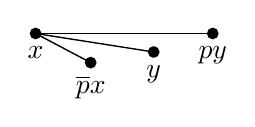
\begin{tikzpicture}
\drinkerbase
\end{tikzpicture}\vspace{1ex}\end{center}
%
%
\end{example}

\begin{lemma}
  If $A$ is a rectified formula then $\graphof A$ is a fograph.
\end{lemma}

\begin{proof}
  That $\graphof A$ is a logical cograph follows immediately from the definition and Theorem~\ref{thm:cograph}.
  The fact that every binder of $\graphof A$ is legal can be proved by
  structural induction on $A$.
  %% :
  %% \begin{itemize}
  %%   \item Trivial if $A$ is an atom.
  %%   \item The induction step uses the following fact:
  %%         if $M$ is a module of $\gG$ and $M' \subseteq M$, then $M'$ is a
  %%         module of $\gG$ if and only if it is a module of $\gG[X]$.
  %% \end{itemize}
  %% \todo{}\lutz{maybe mention also fn 2-5 in Dominic's arxiv-paper}
\end{proof}
%%\juihsuan{I'm still looking for a simple proof}
%
\begin{remark}
Note that $\graphof A$ is not necessarily a fograph if $A$ is not
rectified. If $A = (\forall x. p(x)) \vlor (\forall x. q(x))$, then
$\graphof A = \single x \ \single p(x) \ \single x \ \single q(x)$,
the scope of each $x$-binder contains all the vertices, in particular,
the other $x$-binder. On the other hand, there are non-rectified
formulas which are translated to fographs by $\graphof\cdot$. For
example, in the graph of $(\exists x. p(x)) \vlor (\exists x. q(x))$,
both $x$-binders are legal, as they are not in each other's
scope:
$\edgepairpic{x}{px}\mkern9mu\edgepairpic{x}{qx}$.
\end{remark}
%
%% For this reason, we call a formula
%% \bfit{clean} if it does not contain subformulas of the form $(\forall
%% x.A)\vlor(\forall x.B)$ or $(\exists x.A)\vlan(\exists x.B)$,
%% \todo{need the four cases as in clear definition in fopws? Consider
%% $(\forall x.A)\vlor(B\vlor (\forall x.C))$. But then Lemma 6 doesn't hold.
%% (fopws proves only that there's a surjection from clear formulas onto fographs,
%% whose kernel is the six formula equalities)} and no
%% $x$-quantified formula occurs as subformula of another $x$-quantified
%% formula. Then we have:
%
%% \begin{lemma}
%%   If $A$ is clean iff\/ $\graphof A$ is a fograph.
%% \end{lemma}
%
%% \begin{proof}
%%   Induction on $A$, using  Theorem~\ref{thm:cograph}.
%% \end{proof}
%
%% Even though for every formula $A$ we can obtain an
%% equivalent clean formula by simply renaming some bound variables, this
%% is not unique up to $\alpha$-conversion, as is the case for
%% rectified formulas.
%
\noindent We define a congruence relation $\fequ$ on formulas by the following equations:
\begin{equation}
  \label{eq:fequ}
  \begin{array}{c@{\hskip1.5em}c}
    A \vlan B \fequ B \vlan A
    &
    (A \vlan B) \vlan C \fequ A \vlan (B \vlan C) 
    \\
    A \vlor B \fequ B \vlor A
    &
    (A \vlor B) \vlor C \fequ A \vlor (B \vlor C)
    \\
    \forall x . \forall y . A \fequ \forall y . \forall x . A
    &
    \forall x . (A \vlor B) \fequ (\forall x . A) \vlor B
    \\
    \exists x . \exists y . A \fequ \exists y . \exists x . A
    &
    \exists x . (A \vlan B) \fequ (\exists x . A) \vlan B
  \end{array}
\end{equation}
where $x \notin fv(B)$ in the last two equations.
\todo{Define $fv$; used later too, e.g.\ proof of Lem.\,\ref{lem:me}}
Two formulas $A$ and $B$ are \bfit{equivalent} if $A \fequ B$. The following
theorem shows that the set of fographs can been seen as the quotient
$\FORM/\mathord\fequ$.
\begin{thm}
  Let $A,B$ be rectified formulas. Then
  $$
  A\fequ B \iff \graphof A =\graphof B
  $$
\end{thm}

\begin{proof}
  By a straightforward induction on $A$.
\end{proof}

\begin{example}
  Both $\veedrinkerformula$ and $\variantveedrinkerformula$, which are
  equivalent modulo $\fequ$, have the same (rectified) fograph
  $\drinkergraph$, shown below-left.
  %
  \begin{equation*}
      \drinkergraphpic
      %
      \hspace{8ex}
      %
      \drinkercotreepic
      %
      \hspace{8ex}
      %
      \drinkerbindinggraphpic
  \end{equation*}
  Above-left we show the \emph{cotree} of the underlying
  cograph (illustrating the idea behind Theorem~\ref{thm:cograph}) and
  above-right is its binding graph $\bD$.
\end{example}


%%%%%%%%%%%%%%%%%%%%%%%%%%%%%%%%%%%%%%%%%%%%%%%%%%%%%%%%%%%%%%%%%%%%%%%%%%
%%%%%%%%%%%%%%%%%%%%%%%%%%%%%%%%%%%%%%%%%%%%%%%%%%%%%%%%%%%%%%%%%%%%%%%%%%
%%%%%%%%%%%%%%%%%%%%%%%%%%%%%%%%%%%%%%%%%%%%%%%%%%%%%%%%%%%%%%%%%%%%%%%%%%
%%%%%%%%%%%%%%%%%%%%%%%%%%%%%%%%%%%%%%%%%%%%%%%%%%%%%%%%%%%%%%%%%%%%%%%%%%




\section{First-order Combinatorial Proofs}\label{sec:focp}

%%%%%%%%%%%%%%%%%%%%%%%%%%%%%%%%%%%%%%%%%%%%%%%%%%%%%%%%%%%%
%%%%%%%%%%%%%%%%%%%%%%%%%%%%%%%%%%%%%%%%%%%%%%%%%%%%%%%%%%%%

\subsection{Fonets}

Two atoms are \bfit{pre-dual} if their predicate symbols are dual
(e.g. $p(x, y)$ and $\dual{p}(y, z)$) and two literals are \bfit{pre-dual} if their
labels (atoms) are pre-dual. A \bfit{linked fograph} $\tuple{\gC,\linkingof\gC}$ is a coloured fograph $\gC$ such
that every colour (i.e., equivalence class of~$\linkingof\gC$), called a \bfit{link}, consists of two pre-dual literals, and
every literal is either $\ttt$-labelled or in a link.

Let $\gC$ be a linked fograph. The set of links can be seen as a unification problem
by identifying dual predicate symbols. A \bfit{dualizer} of $\gC$ is a substitution $\delta$
unifying all the links of~$\gC$. Since a first-order unification problem is either
unsolvable or has a most general unifier, we can define the notion of \bfit{most
general dualizer}. A \bfit{dependency} is a pair $\set{\single x, \single y}$ of an
existential binder $\single x$ and a universal binder $\single y$ such that the most
general dualizer assigns to $x$ a term containing $y$. A \bfit{leap} is either a
link or a dependency. The \bfit{leap graph} $\lgC$ of $\gC$ is the undirected
graph $\tuple{\vC, \lpC}$ where $\lpC$ is the set of leaps of $\gC$.
A vertex set $W \subseteq \vC$ induces a \bfit{matching} in
$\gC$ if 
it is non-empty\dominic{added non-empty (necessary, right?)}
for all $w \in W$, $N(w) \cap W$ is a singleton. We say that $W$ induces a
\bfit{bimatching} in $\gC$ if it induces a matching in $\gC$ and a matching in $\lgC$.


\begin{definition}
A \bfit{first-order net} or \bfit{fonet} is a linked fograph which
has a dualizer but no induced bimatching.  
\end{definition}
%
\begin{figure}[!t]
  \begin{center}
    \vspace{-1ex}
    \begin{tikzpicture}[graph]
      \begin{scope}[xshift=-2.2cm]\twolinkfograph\end{scope}
        \begin{scope}[xshift=2.2cm]\twolinkleapgraph\end{scope}
    \end{tikzpicture}\vspace{-4ex}
  \end{center}%
  \caption{\label{fig:leap}A fonet (left) with
    dualizer $\protect\twolinkassignment$
    and its
    leap graph (right).}
\end{figure}%
%
Figure~\ref{fig:leap} shows a fonet with a unique dualizer, and its leap graph.

%%%%%%%%%%%%%%%%%%%%%%%%%%%%%%%%%%%%%%%%%%%%%%%%%%%%%%%%%%%%
%%%%%%%%%%%%%%%%%%%%%%%%%%%%%%%%%%%%%%%%%%%%%%%%%%%%%%%%%%%%

\begin{figure*}
  $$
  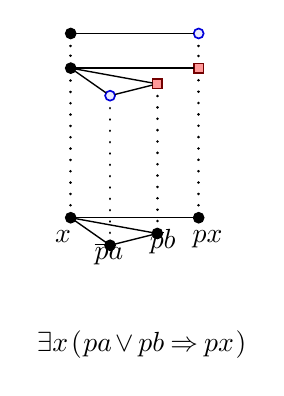
\begin{tikzpicture}\cponeonformula
  \end{tikzpicture}
  \qquad
  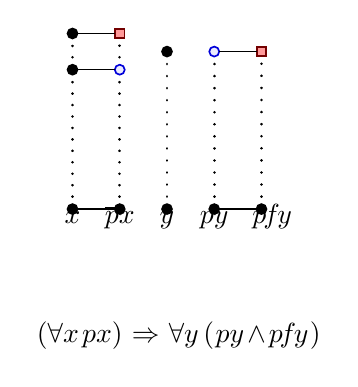
\begin{tikzpicture}\cptwoonformula
  \end{tikzpicture}
  \qquad
  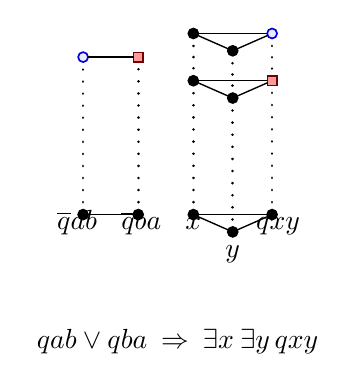
\begin{tikzpicture}\cpthreeonformula
  \end{tikzpicture}
  \qquad
  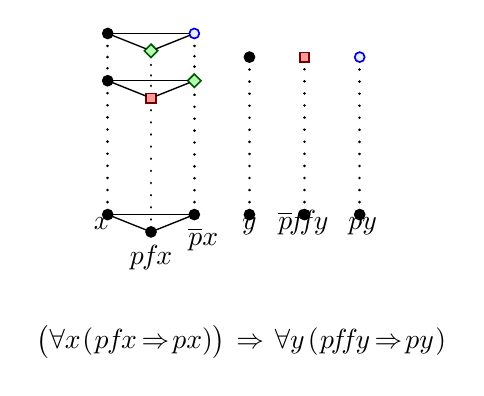
\begin{tikzpicture}\cpfouronformula
  \end{tikzpicture}
  $$
  \vskip-2ex
  \caption{Four combinatorial proofs, each shown
    above the formula proved.  Here $x$ and $y$ are variables, $f$ is
    a unary function symbol, $a$ and $b$ are constants (nullary
    function symbols), $p$ is a unary predicate symbol, and $q$ is a
    binary predicate symbol.}
  \label{fig:cps}
\end{figure*}

\begin{figure*}
  $$
  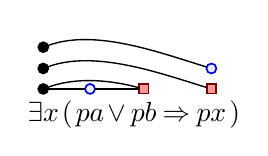
\begin{tikzpicture}
    \cponeinline
  \end{tikzpicture}
  \qquad\;
  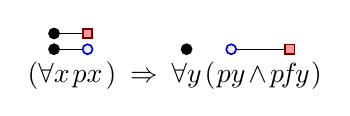
\begin{tikzpicture}
    \cptwoinline
  \end{tikzpicture}
  \qquad\;
  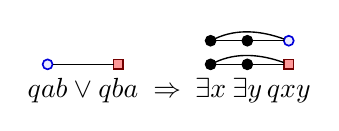
\begin{tikzpicture}
    \cpthreeinline
  \end{tikzpicture}
  \qquad\;
  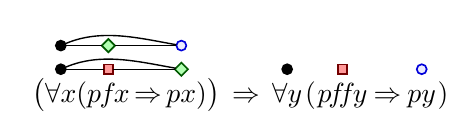
\begin{tikzpicture}
    \cpfourinline
  \end{tikzpicture}
  $$
  \vskip-2ex
  \caption{Condensed forms of the four combinatorial proofs in Fig.\,\ref{fig:cps}.}
  \label{fig:cps-condensed}
  %\vspace{-4ex}
\end{figure*}

\subsection{Skew Bifibrations}

A graph homomorphism $\phi\colon \tuple{\vG, \eG} \rightarrow
\tuple{\vH, \eH}$ is a \bfit{fibration} if for all $v \in \vG$ and
$w\phi(v) \in \eH$, there exists a unique $\tilde{w} \in \vG$ such
that $\tilde{w}v \in \eG$ and $\phi(\tilde{w}) = w$ (indicated below-left),
and is a
\bfit{skew fibration} if for all $v \in \vG$ and $w\phi(v) \in \eH$
there exists $\tilde{w} \in \vG$ such that $\tilde{w}v \in \eG$ and
$\phi(\tilde{w})w \notin \eH$ (indicated below-centre).
A directed graph homomorphism is a
\bfit{fibration} if for all $v \in \vG$ and $\pair{w,\phi(v)} \in
\eH$, there exists a unique $\tilde{w} \in \vG$ such that $\pair{\tilde{w},v}
\in \eG$ and $\phi(\tilde{w}) = w$ (indicated below-right).
%
\liftingdiagrams
%
A \bfit{fograph homomorphism} $\phi=\tuple{\phi,\rsubstof\phi}$ is a
pair where $\phi\colon\gG\to\gH$ is a graph homomorphism between the
underlying graphs, and $\rsubstof\phi$, also called the
\bfit{substitution induced by $\phi$} is a variable renaming 
such that
for all $v\in\vG$ we have
$\labelof{\phi(v)}=\rsubstof\phi(\labelof v)$,
and $\rsubstof\phi$ is the identity on variables not in $\gG$.
%
Note that $\phi$ necessarily maps binders to binders
and literals to literals.
%
Since $\rsubstof\phi$ is fully determined by $\phi$ alone, we often
leave $\rsubstof\phi$ implicit.
A fograph homomorphism $\phi\colon\gG \rightarrow \gH$
%%\bfit{label-preserving} if for all $v \in \vG, label(v) = label(f(v))$, and is
% is \bfit{existential-preserving} 
\bfit{preserves existentials}
if for all existential binders $b$ in
$\gG$, the binder $\phi(b)$ is a existential in $\gH$.\dominic{tweaked this paragraph}
%
\begin{definition}
  Let $\gG$ and $\gH$ be fographs. A \bfit{skew bifibration}
  $\phi\colon\gG\to\gH$ is an existential-preserving fograph
  homomorphism that is a skew fibration on $\tuple{\vG, \eG} \to
  \tuple{\vH, \eH}$ and a fibration on the binding graphs $\bG\to\bH$.
  %etween fographs is a label-preserving and
%existential-preserving fograph homomorphism whose restriction to the
%binding graphs is a fibration.
\end{definition}
%
\begin{example}
  Below-left is a skew bifibration, whose binding fibration
  is below-centre. When the labels on the source fograph can be inferred
  (modulo renaming),
  we often omit the labeling in the upper graph, as below-right, which refer to as 
  \bfit{condensed form}.\dominic{I said ``can be inferred'' to account for 
  e.g.\
  $\graphof{\forall x_1\forall x_2 (px_i\vee px_j\vee px_k\vee px_l)}
  \to \graphof{\forall x\mkern2mu px}$ whose
  unlabelled skeleton is the skeleton of many distinct formula variants (``who binds who?'').}
  \begin{center}\begin{math}
  \scalebox{.9}{
  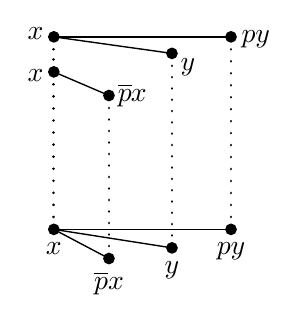
\begin{tikzpicture}[graph]\drinkerfiblabelledpair{x}{x}
  \end{tikzpicture}
  \quad
  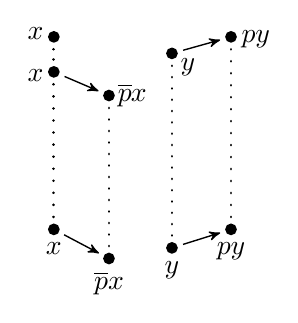
\begin{tikzpicture}[graph]\drinkerbindingfiblabelled{x}{x}
  \end{tikzpicture}
  \quad
  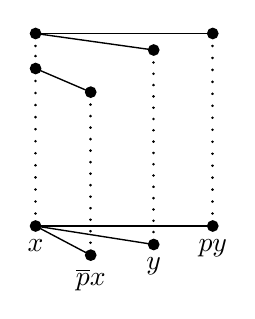
\begin{tikzpicture}[graph]\drinkerfib
  \end{tikzpicture}}
\end{math}\end{center}\end{example}
%
%%\subsection{First-order combinatorial proofs}
%
\begin{definition}
A \bfit{first-order combinatorial proof} (\bfit{FOCP}) of a fograph $\gG$ is a skew
bifibration $\phi\colon \gC \rightarrow \gG$ where $\gC$ is a fonet. A \bfit{first-order
combinatorial proof} of a formula $A$ is a combinatorial proof of its graph
$\graphof{A}$.
\end{definition}
%
Figure~\ref{fig:cps} shows examples of
FOCPs (taken from~\cite{hughes:fopws}), each above the formula it proves.
The same FOCPs are shown in
Figure~\ref{fig:cps-condensed} in condensed form.
%
\begin{thm}[\cite{hughes:fopws}]
  \label{thm:FOCP}
  FOCPs are sound and complete for first-order logic.
\end{thm}
%
\begin{remark}
  Our definition of FOCP is slightly more lax than the original
  definition of~\cite{hughes:fopws}, as we allow for a variable
  renaming $\substof\phi$ which was forced to be the identity
  in~\cite{hughes:fopws}.
  %The reason for this relaxation in our case is that we want to cover a richer class of proofs, also allowing 
\end{remark}

%%%%%%%%%%%%%%%%%%%%%%%%%%%%%%%%%%%%%%%%%%%%%%%%%%%%%%%%%
%%%%%%%%%%%%%%%%%%%%%%%%%%%%%%%%%%%%%%%%%%%%%%%%%%%%%%%%%
%%%%%%%%%%%%%%%%%%%%%%%%%%%%%%%%%%%%%%%%%%%%%%%%%%%%%%%%%
%%%%%%%%%%%%%%%%%%%%%%%%%%%%%%%%%%%%%%%%%%%%%%%%%%%%%%%%%


\section{First-order Deep Inference system $\FOKS$}\label{sec:foks}


\begin{figure}
  \begin{center}
    \framebox{%
      $
      \begin{array}{@{}c@{}}
        \dbox{%
          $
          \begin{array}{c}
            \vlinf{\faD}{}{\Scons{\forall x.\ttt}}{\Scons\ttt}
            \qquad
            \vlinf{\aiD}{}{\Scons{a\vlor\cneg a}}{\Scons\ttt}
            \qquad
            \vlinf{\tttD}{}{\Scons{A\vlan\ttt}}{\Scons A}
            \\ \\[-1ex]
            \vlinf{\sw}{}{\Scons{(A\vlan B)\vlor C}}{\Scons{A\vlan (B\vlor C)}}
            \qquad
            \vlinf{\mix}{}{\Scons{A\vlor B}}{\Scons{A\vlan B}}            
            \\ \\[-1ex]
            \vlinf{\exD}{}{\Scons{\exists x.A}}{\Scons{A\ssubst x t}}
            \qquad
            \vlinf{\fequ}{\text{(where $A\fequ B$)}}{\Scons{A}}{\Scons{B}}
          \end{array}
          $
        }
        \\ \\[-1ex]
        \vlinf{\mfaD}{}{\Scons{\forall x.(A\vlor B)}}{\Scons{(\forall x.A)\vlor(\forall x.B)}}
        \qquad
        \vlinf{\mexD}{}{\Scons{\exists x.(A\vlor B)}}{\Scons{(\exists x.A)\vlor(\exists x.B)}}        
        \\ \\[-1ex]
        \vlinf{\me}{}{\Scons{(A\vlor B)\vlan(C\vlor D)}}{\Scons{(A\vlan C)\vlor(B\vlan D)}}
        \\ \\[-1ex]
        \vlinf{\wrD}{}{\Scons{A\vlor B}}{\Scons{A}}
        %%\qquad
        %%\vlinf{\wlD}{}{\Scons{B\vlor A}}{\Scons{A}}
        \qquad
        \vlinf{\acD}{}{\Scons{a}}{\Scons{a\vlor a}}
        \qquad
        \vlinf{\cfaD}{}{\Scons{\forall x. A}}{\Scons{\forall x.\forall x.A}}
      \end{array}
      $
    }
  \end{center}
  \caption{Deep inference systems $\FOKS$ (all rules) and $\FOMLS$ (rules in the dashed box)}
  \label{fig:KS1}
\end{figure}
%
In contrast to to standard proof formalisms, like sequent calculi or
tableaux, where inference rules decompose the principal formula along
its root connective, \emph{deep inference rules} apply like
rewriting rules inside any (positive) formula or sequent
\bfit{context}, which is denoted as $\Sconhole$, and which is a
formula (resp.~sequent) with exactly one occurrence of the \bfit{hole}
$\conhole$ in the position of an atom. Then $\Scons A$ is the result
of replacing the hole $\conhole$ in $\Sconhole$ with $A$.

Figure~\ref{fig:KS1} shows the inference rules for the deep inference
system~$\FOKS$ that we introduce in this paper. It is a slight variation
of the systems presented by Br\"unnler~\cite{brunnler:phd} and
Ralph~\cite{ralph:phd} in their PhD-theses. The main differences are
(i) the explicit presence of the $\mixr$-rule, (ii) a
different choice of how the formula equivalence $\fequ$ is defined,
and (iii) an explicit rule for the equivalence.

We consider here only the cut-free fragment, as cut-elimination for
deep inference systems has already been discussed
elsewhere (e.g.~\cite{brunnler:06:herbrand,alertubella:guglielmi:18}).%
%\juihsuan{references added. Please check if they are the right ones.}
\footnote{In the deep
inference literature, the cut-free fragment is also called the
\emph{down-fragment}. But as we do not discuss the \emph{up-fragment}
here, we omit the down-arrows $\downarrow$ in the rule names.}

As with the sequent system $\FOLK$, we also need for $\FOKS$ the
\emph{linear fragment}, $\FOMLS$, and that is shown
in Figure~\ref{fig:KS1} in the dashed box.

Write $\vlder{\sysS}{\Deri}{A}{B}$ to denote a derivation $\Deri$
from $B$ to $A$ using the rules from system $\sysS$. A formula $A$ is
\bfit{provable} in a system $\sysS$ if there is a derivation in
$\sysS$ from $\ttt$ to $A$.

In the course of this paper we will employ the
general (non-atomic) version of the contraction rule:
\begin{equation*}
  \vlinf{\cD}{}{\Scons{A}}{\Scons{A\vlor A}}  
\end{equation*}

%%%%%%%%%%%%%%%%%%%%%%%%%%%%%%%%%%%%%%%%%%%%%%%%%%%%%%%%%
%%%%%%%%%%%%%%%%%%%%%%%%%%%%%%%%%%%%%%%%%%%%%%%%%%%%%%%%%
%%%%%%%%%%%%%%%%%%%%%%%%%%%%%%%%%%%%%%%%%%%%%%%%%%%%%%%%%
%%%%%%%%%%%%%%%%%%%%%%%%%%%%%%%%%%%%%%%%%%%%%%%%%%%%%%%%%


\section{Main Results}
\label{sec:main}

We state the main results of this paper here,
and prove them in later sections. The
first is routine and expected, but needs to be proved nonetheless:

\begin{thm}\label{thm:KS1}
  $\FOKS$ is sound and complete for first-order logic.
\end{thm}

Our second result is more surprising, as it is a very strong
decomposition result for first order logic.

\begin{thm}\label{thm:decomposition}
  For every derivation $\vlder{\FOKS}{\Deri}{A}{\ttt}$ there are formulas $A_1,\ldots,A_5$, such that there is a derivation:
  \begin{equation*}
    \vlderivation{
      \vlde{\set{\wrD,\fequ}}{}{A}{
        \vlde{\set{\acD,\cfaD}}{}{A_1}{
          \vlde{\set{\me,\mfaD,\mexD,\fequ}}{}{A_2}{
            \vlde{\set{\exD}}{}{A_3}{
              \vlde{\set{\sw,\mix,\fequ}}{}{A_4}{
                \vlde{\set{\faD,\aiD,\tttD}}{}{A_5}{
                  \vlhy{\ttt}}}}}}}}
  \end{equation*}
\end{thm}

This theorem is stronger than the existing decompositions for
first-order logic, which either separated only atomic contraction and
atomic weakening~\cite{brunnler:phd} or only
contraction~\cite{ralph:phd} or only the quantifiers in form of a
Herbrand theorem~\cite{brunnler:06:locality,ralph:phd}.

\begin{example}
  Below is an example of a decomposed derivation in $\FOKS$ of the
  formula $(\exists x. \cneg{p}(x)) \vlor (\forall y.(p(y) \vlan
  p(f(y))))$:
  \begin{equation*}
    \vlderivation{
      \vlin{\acD}{}{(\exists x. \cneg{p}x) \vlor (\forall y.(py \vlan pfy))}{
        \vlin{\mexD}{}{(\exists x. (\cneg{p}x \vlor \cneg{p}x) \vlor (\forall
          y.(py \vlan pfy))}{
          \vlin{\fequ}{}{((\exists x. \cneg{p}x) \vlor (\exists x.\cneg{p}x))
            \vlor (\forall y.(py \vlan pfy)}{
            \vlin{\exists}{}{\forall y.(((\exists x. \cneg{p}x) \vlor (\exists
              x.\cneg{p}x)) \vlor (py \vlan pfy))}{
              \vlin{\exists}{}{\forall y.((\cneg{p}y \vlor (\exists x.\cneg{p}x))
                \vlor (py \vlan pfy))}{
                \vlin{\fequ}{}{\forall y.((\cneg{p}y \vlor \cneg{p}fy) \vlor
                  (py \vlan pfy))}{
              \vlin{\sw}{}{\forall y.(\cneg{p}y \vlor ((py \vlan pfy)
                \vlor \cneg{p}fy))}{
                \vlin{\fequ}{}{\forall y.(\cneg{p}y \vlor (py \vlan (pfy
                  \vlor \cneg{p}fy)))}{
                  \vlin{\aiD}{}{\forall y.((\cneg{p}y \vlor py) \vlan (pfy
                    \vlor \cneg{p}fy))}{
                    \vlin{\aiD}{}{\forall y.((\cneg{p}y \vlor py) \vlan
                      \ttt)}{
                      \vlin{\ttt}{}{\forall y.(\ttt \vlan \ttt)}{
                        \vlin{\forall}{}{\forall y.\ttt}{
                          \vlhy{\ttt}}}}}}}}}}}}}}
  \end{equation*}
\end{example}
%
There is a weaker version of Theorem~\ref{thm:decomposition} that will
also be useful:
%
\begin{thm}\label{thm:decompositionA}
  For every derivation $\vlder{\FOKS}{\Deri}{A}{\ttt}$ there is a formula $A_1$, such that there is a derivation:
  \begin{equation*}
    \vlderivation{
      \vlde{\set{\wrD,\cD,\fequ}}{}{A}{
        \vlde{\FOMLS}{}{A_1}{
          \vlhy{\ttt}}}}
  \end{equation*}
\end{thm}

Let us now establish the connection between derivations in $\FOKS$ and
combinatorial proofs.

\begin{thm}\label{thm:CP-DI}
  Let  $\phi\colon\gC\to\gA$ be a combinatorial proof and let $A$ be a formula with $\gA=\graphof A$. Then there is a derivation
  \begin{equation}
    \label{eq:decom}
    \vlderivation{
      \vlde{\set{\wrD,\acD,\cfaD,\me,\mfaD,\mexD,\fequ}}{\Deri_2}{A}{
        \vlde{\FOMLS}{\Deri_1}{A'}{
          \vlhy{\ttt}}}}
  \end{equation}
  for some $A'\fequ C\substof\phi$ where $C$ is a formula with $\graphof
  C=\gC$ and $\substof\phi$ is the variable renaming substitution
  induced by~$\phi$.  Conversely,
  whenever we have a derivation as in~\eqref{eq:decom} above, then
  there is a combinatorial proof $\phi\colon\gC\to\graphof A$ such
  that $\gC=\graphof{\rectif{A'}}$.
\end{thm}

Furthermore, in the proof of Theorem~\ref{thm:CP-DI}, we will see that
(i) the links in the fonet $\gC$ correspond precisely to the pairs of
atoms that meet in the instances of the $\aiD$-rule in the derivation
$\Deri_1$, and (ii) the ''flow-graph'' of $\Deri_2$ that traces the
quantifier- and atom-occurrences in the derivation corresponds exactly
to the vertex-mapping induced by $\phi$.

Thus, combinatorial proofs are closely related to derivations of the
form~\eqref{eq:decom}, and since by Theorem~\ref{thm:decomposition}
every derivation can be transformed into that form, we can say that
combinatorial proofs form a canonical proof representation for first
order logic, similarly to what proof nets are for linear
logic~\cite{girard:96:PN}.

Finally, Theorems~\ref{thm:KS1}, \ref{thm:decomposition}
and~\ref{thm:CP-DI} imply Theorem~\ref{thm:FOCP}, which means that we
have here an alternative proof of the soundness and completeness of
first-order combinatorial proofs which is simpler than the one given
in~\cite{hughes:fopws}.



%%%%%%%%%%%%%%%%%%%%%%%%%%%%%%%%%%%%%%%%%%%%%%%%%%%%%%%%%
%%%%%%%%%%%%%%%%%%%%%%%%%%%%%%%%%%%%%%%%%%%%%%%%%%%%%%%%%
%%%%%%%%%%%%%%%%%%%%%%%%%%%%%%%%%%%%%%%%%%%%%%%%%%%%%%%%%
%%%%%%%%%%%%%%%%%%%%%%%%%%%%%%%%%%%%%%%%%%%%%%%%%%%%%%%%%

\section{Translating between $\FOLK$ and $\FOKS$}
\label{sec:LK1-KS1}

In this section we prove Theorems~\ref{thm:KS1},
\ref{thm:decomposition}, and~\ref{thm:decompositionA}, mainly by
translating derivations to and from the sequent calculus, and by rule
permutation arguments.

\subsection{The Linear Fragments $\FOMLL$ and $\FOMLS$}

In this section we show the equivalence of $\FOMLL$ and $\FOMLS$.

\begin{lemma}\label{lem:MLL1->MLS1}
  If $\sqn\Gamma$ is provable in $\FOMLL$ then $\form\Gamma$ is provable in  $\FOMLS$.
\end{lemma}

\begin{proof}
  This is a straightforward induction on the proof of $\sqn\Gamma$ in
  $\FOMLL$, making a case analysis on the bottommost rule instance. We
  show here only the case of $\vlinf{\forall}{}{\sqn{\Delta,\forall
      x.A}}{\sqn{\Delta,A}}$ (all other cases are simpler and have
  been shown before, e.g.~\cite{brunnler:phd}): By induction
  hypothesis, there is a proof of $\form\Delta\vlor A$ in $\FOMLS$. We
  can prefix every line in that proof by $\forall x$ and then compose
  the following derivation:
  \begin{center}\vspace{-2ex}\begin{math}
    \vlderivation{
      \vlin{\fequ}{}{\form\Delta\vlor\forall x.A}{
        \vlde{\FOMLS}{}{\forall x.\form\Delta\vlor A}{
          \vlin{\forall}{}{\forall x.\ttt}{
            \vlhy{\ttt}}}}}
  \end{math}\end{center}
  where we can apply the $\fequ$-rule because $x$ is not free in $\Delta$.
\end{proof}

\begin{lemma}\label{lem:shallow}
  Let $\vlinf{\rr}{}{\Scons B}{\Scons A}$ be an inference rule in
  $\FOMLS$ other than $\aiD$. Then the sequent $\sqn{\cneg A,B}$ is provable in $\FOMLL$.
\end{lemma}
\begin{proof}
  This is a straightforward exercise that we leave to the reader. (Note that the
$\ax$-rule can be applied to $\sqn{\fff,\ttt}$ in the cases of $\rr = \faD$.)
\end{proof}

\begin{lemma}\label{lem:context}
  Let $A,B$ be formulas, and let $\Sconhole$ be a (positive)
  context. If $\sqn{\cneg A,B}$ is provable in $\FOMLL$, then so is
  $\sqn{\cneg{\Scons A},\Scons B}$.
\end{lemma}

\begin{proof}
  Straightforward induction on  $\Sconhole$. (see e.g. \cite{gug:str:01})
\end{proof}

\begin{lemma}\label{lem:MLS1->MLL1}
  If a formula $C$ is provable in $\FOMLS$ then $\sqn C$ is provable in  $\FOMLL$. 
\end{lemma}

\begin{proof}
  We proceed by induction on the number of inference steps in the
  proof of $C$ in $\FOMLS$. Consider the bottommost rule instance
  $\vlinf{\rr}{}{\Scons B}{\Scons A}$. By induction hypothesis we have
  a $\FOMLL$ proof $\Proof$ of $\sqn{\Scons A}$. If $\rr$ is
  $\upsmash{\vlinf{\aiD}{}{\Scons{a\vlor\cneg a}}{\Scons\ttt}}$, we replace
  in $\Pi$ all corresponding occurrences of $\ttt$ with
  $a \vlor \cneg a$ and the rule instance
  $\vlinf{\ttt}{}{\sqn{\ttt}}{}$ with the derivation $ \vlderivation{
    \vlin{\vlor}{}{\sqn{a \vlor \cneg a}}{ \vlin{\axr}{}{\sqn{a, \cneg
          a}}{ \vlhy{}}}} $. This gives us a proof of
  $\sqn{\Scons{a \vlor \cneg a}}$. In all other cases, 
    %\item $\vlinf{\faD}{}{\Scons{\forall x.\ttt}}{\Scons\ttt}$
     % In this case, we replace simultaneously in $\Pi$ the corresponding
     % occurrences of $\ttt$ with $\forall x.\ttt$ and the rule instance
     % $\vlinf{\ttt}{}{\sqn{\ttt}}{}$ with the derivation
     % $
     % \vlderivation{
     %   \vlin{\forall}{}{\sqn{\forall x.\ttt}}{
     %     \vlin{\axr}{}{\sqn{\ttt}}{
     %       \vlhy{}}}}
     % $, and we get a proof $\Pi'$ of $\sqn{\Scons{\forall x.\ttt}}$.
      by Lemmas~\ref{lem:shallow} and~\ref{lem:context}, we have a $\FOMLL$ proof of
      $\sqn{\cneg{\Scons A},\Scons B}$. We can compose them via $\cutr$:
      \begin{equation*}
        \vliinf{\cutr}{}{\sqn{\Scons B}}{\sqn{\Scons A}}{\sqn{\cneg{\Scons
          A},\Scons B}}
      \end{equation*}
      and then apply Theorem~\ref{thm:cutelim}.
  \end{proof}

%%%%%%%%%%%%%%%%%%%%%%%%%%%%%%%%%%%%%%%%%%%%%%%%%%%%%%%%%
%%%%%%%%%%%%%%%%%%%%%%%%%%%%%%%%%%%%%%%%%%%%%%%%%%%%%%%%%
\subsection{Contraction and Weakening}

The first observation here is that Lemmas~\ref{lem:MLL1->MLS1}--\ref{lem:MLS1->MLL1} from above also hold for $\FOLK$ and $\FOKS$. We therefore immediately have:

\begin{thm}\label{thm:LK1-KS1}
  For every sequent $\Gamma$, we have that $\sqn\Gamma$ is provable in
  $\FOLK$ if and only if $\form\Gamma$ is provable in $\FOKS$.
\end{thm}

Then Theorem~\ref{thm:KS1} is an immediate consequence. Let us now
proceed with providing further lemmas that will be needed for the
other results.

\begin{lemma}
  \label{lem:ac}
  The $\cD$-rule is derivable in $\set{\acD,\me,\mfaD,\mexD,\fequ}$. 
\end{lemma}

\begin{proof}
  We show that there is always a derivation
  $$
  \vlderivation{
    \vlde{\sysS}{}{A}{
      \vlhy{A \vlor A}}}
  $$, where $\sysS = \set{\acD,\me,\mfaD,\mexD,\fequ}$, by induction on $A$:
  \begin{itemize}
    \item If $A = a$, then we have
      $
      \vlderivation{
        \vlin{\acD}{}{a}{
          \vlhy{a \vlor a}}}
      $.
    \item If $A = B \vlan C$, then we have
      $
      \vlderivation{
	\vlde{\sysS}{}{B \vlan C}{
	  \vlde{\sysS}{}{B \vlan (C \vlor C)}{
	    \vlin{\me}{}{(B \vlor B) \vlan (C \vlor C)}{
	      \vlhy{(B \vlan C) \vlor (B \vlan C)}}}}}
      $.\\[.5ex]
    \item If $A = B \vlor C$, then we have
      $
      \vlderivation{
	\vlde{\sysS}{}{B \vlor C}{
	  \vlde{\sysS}{}{B \vlor (C \vlor C)}{
	    \vlin{\fequ}{}{(B \vlor B) \vlor (C \vlor C)}{
	      \vlhy{(B \vlor C) \vlor (B \vlor C)}}}}}
      $.\\[.5ex]
    \item If $A = \exists x.A'$, then we have
      $
      \vlderivation{
	\vlde{\sysS}{}{\exists x.A'}{
	  \vlin{\mexD}{}{\exists x.(A' \vlor A')}{
	    \vlhy{(\exists x.A') \vlor (\exists x.A')}}}}
      $.\\[.5ex]
    \item If $A = \forall x.A'$, then we have
      $
      \vlderivation{
	\vlde{\sysS}{}{\forall x.A'}{
	  \vlin{\mexD}{}{\forall x.(A' \vlor A')}{
	    \vlhy{(\forall x.A') \vlor (\forall x.A')}}}}
      $.
  \end{itemize}
  \todo{}
  \juihsuan{done. Maybe just keep one case.}\lutz{yes, but we do that at the end. don't think about space right now.}
\end{proof}

\begin{lemma}
  \label{lem:me}
  $\cfaD,\me,\mfaD,\mexD$ are derivable in \hbox{$\set{\wrD,\cD,\fequ}$}. 
\end{lemma}

\begin{proof}
  \todo{}

  We have the following derivations:
  $$
  \vlderivation{
    \vlin{\cD}{}{\forall x.A}{
      \vlin{\equiv}{(x \notin fv(\forall x.A))}{(\forall x.A) \vlor (\forall x.A)}{
        \vlin{\wrD}{}{\forall x.((\forall x.A) \vlor A)}{
          \vlhy{\forall x.\forall x.A}}}}}
  $$.
  $$
  \vlderivation{
    \vlin{\cD}{}{(A \vlor B) \vlan (C \vlor D)}{
      \vlin{\fequ}{}{((A \vlor B) \vlan (C \vlor D)) \vlor ((A \vlor B) \vlan (C \vlor D))}{
      \vlin{\wrD}{}{((A \vlor B) \vlan (C \vlor D)) \vlor ((B \vlor A) \vlan (D \vlor C))}{
	\vlin{\wrD}{}{((A \vlor B) \vlan (C \vlor D)) \vlor ((B \vlor A) \vlan D))}{
	  \vlin{\wrD}{}{((A \vlor B) \vlan (C \vlor D)) \vlor (B \vlan D))}{
	    \vlin{\wrD}{}{((A \vlor B) \vlan C) \vlor (B \vlan D)}{
	      \vlhy{(A \vlan C) \vlor (B \vlan D)}}}}}}}}
  $$.
  $$
  \vlderivation{
    \vlin{\cD}{}{\exists x.(A \vlor B)}{
      \vlin{\fequ}{}{\exists x.(A \vlor B)) \vlor (\exists x.(A \vlor B))}{
      \vlin{\wrD}{}{(\exists x.(A \vlor B)) \vlor (\exists x.(B \vlor A))}{
	\vlin{\wrD}{}{(\exists x.(A \vlor B)) \vlor (\exists x.B)}{
	  \vlhy{(\exists x.A) \vlor (\exists x.B)}}}}}}
  $$.
  $$
  \vlderivation{
    \vlin{\cD}{}{\forall x.(A \vlor B)}{
      \vlin{\fequ}{}{(\forall x.(A \vlor B)) \vlor (\forall x.(A \vlor B))}{
      \vlin{\wrD}{}{(\forall x.(A \vlor B)) \vlor (\forall x.(B \vlor A))}{
	\vlin{\wrD}{}{(\forall x.(A \vlor B)) \vlor (\forall x.B)}{
	  \vlhy{(\forall x.A) \vlor (\forall x.B)}}}}}}
  $$.
  \juihsuan{done. If needed, we can introduce the notion of open deduction to
reduce the size of derivations...}\lutz{I was thinking about that, but (i) it is probably not worth the effort, as we wont have many derivation, and (ii) it is hard to define rectified derivations this way.}
\end{proof}

\begin{lemma}
  Let $A$ and $B$ be formulas. Then
  \begin{equation*}
    \vlderivation{
      \vlde{\set{\wrD,\cD,\fequ}}{}{B}{
        \vlhy{A}}}
    \qquad
    \iff
    \qquad
    \vlderivation{
      \vlde{\set{\wrD,\acD,\cfaD,\me,\mfaD,\mexD,\fequ}}{}{B}{
        \vlhy{A}}}
  \end{equation*}
\end{lemma}

\begin{proof}
  This follows immediately from Lemmas~\ref{lem:ac} and~\ref{lem:me}.
\end{proof}

%%%%%%%%%%%%%%%%%%%%%%%%%%%%%%%%%%%%%%%%%%%%%%%%%%%%%%%%%
%%%%%%%%%%%%%%%%%%%%%%%%%%%%%%%%%%%%%%%%%%%%%%%%%%%%%%%%%
\subsection{Rule Permutations}

%All statements in this section are proved by rule permutation arguments.
\begin{thm}\label{thm:LK1-decompose}
  Let $\Gamma$ be a sequent. If\/ $\sqn\Gamma$ is provable in $\FOLK$ (as depicted on the left below) then there is a sequent
  $\Gamma'$ such that there is a derivation as shown on the right below:\vadjust{\vskip-2ex}
  \begin{equation*}
    \vlderivation{
        \vltrl{}{\FOLK}{\Deri}{\sqns{\Gamma}}{
          \vlhy{\quad}}{
          \vlhy{}}{
          \vlhy{}}}
    \qquad
    \Longrightarrow
    \qquad
    \vlderivation{
      \vlde{\set{\wrD,\cD,\fequ}}{\Deri_2}{\sqns{\form{\Gamma}}}{
        \vltrl{}{\FOMLL}{\Deri_1}{\sqns{\Gamma'}}{
          \vlhy{\quad}}{
          \vlhy{}}{
          \vlhy{}}}}
  \end{equation*}
\end{thm}

\begin{proof}

  Note that the instances of $\wrD,\cD$ in $\Deri_2$ are deep, but inside sequent contexts.

First, if an instance of $\vlinf{\weakr}{}{\sqn{\Gamma,A}}{\sqn{\Gamma}}$
 is followed by a rule in which $A$ is not in the principal
formula, it can be permuted downwards.
Otherwise, the proof can be transformed using the following rewriting rules.

\begin{equation*}
\vlderivation{
  \vliin{\vlan}{}{\sqns{\Gamma, A \vlan B, \Delta}}{
    \vlin{\weakr}{}{\sqns{\Gamma, A}}{
      \vlhy{\sqns{\Gamma}}}}{
    \vlhy{\sqns{B, \Delta}}}}
\leadsto
\vlderivation{
  \vlin{\weakr}{}{\sqns{\Gamma, A \vlan B, \Delta}}{
    \vlin{\weakr}{}{\vlvdots}{
      \vlhy{\sqns{\Gamma}}}}}
\end{equation*}
\begin{equation*}
\vlderivation{
  \vlin{\vlor}{}{\sqns{\Gamma, A \vlor B}}{
    \vlin{\weakr}{}{\sqns{\Gamma, A, B}}{
      \vlhy{\sqns{\Gamma, A}}}}}
\leadsto
\vlderivation{
  \vlin{\wrD}{}{\sqns{\Gamma, A \vlor B}}{
    \vlhy{\sqns{\Gamma, A}}}}
\end{equation*}
\begin{equation*}
\vlderivation{
  \vlin{\exists}{}{\sqns{\Gamma, \exists x.A}}{
    \vlin{\weakr}{}{\sqns{\Gamma, A\ssubst{x}{t}}}{
      \vlhy{\sqns{\Gamma}}}}}
\leadsto
\vlderivation{
  \vlin{\weakr}{}{\sqns{\Gamma, \exists x.A}}{
    \vlhy{\sqns{\Gamma}}}}
\end{equation*}
\begin{equation*}
\vlderivation{
  \vlin{\forall}{}{\sqns{\Gamma, \forall x.A}}{
    \vlin{\weakr}{}{\sqns{\Gamma, A}}{
      \vlhy{\sqns{\Gamma}}}}}
\leadsto
\vlderivation{
  \vlin{\weakr}{}{\sqns{\Gamma, \forall x.A}}{
    \vlhy{\sqns{\Gamma}}}}
\end{equation*}
\begin{equation*}
\vlderivation{
  \vlin{\conr}{}{\sqns{\Gamma, A}}{
    \vlin{\weakr}{}{\sqns{\Gamma, A, A}}{
      \vlhy{\sqns{\Gamma, A}}}}}
\leadsto
\vlderivation{
  \vlhy{\sqns{\Gamma, A}}}
\end{equation*}
Note that in the case of $\vlor$, we use the deep rule $\wrD$ which can be
permuted down over all the rules. By using these rewriting rules, we can eventually get
a derivation with all the instances of $\weakr$ and $\wrD$ at the bottom. Now observe
that the instances of $\conr$ in $\Deri$ can be transformed using the following
rule:

\begin{equation*}
\vlderivation{
  \vlin{\conr}{}{\sqns{\Gamma, A}}{
    \vlhy{\sqns{\Gamma, A, A}}}}
\leadsto
\vlderivation{
  \vlin{\cD}{}{\sqns{\Gamma, A}}{
    \vlin{\vlor}{}{\sqns{\Gamma, A \vlor A}}{
      \vlhy{\sqns{\Gamma, A, A}}}}}
\end{equation*}

Knowing that $\cD$ can be permuted down over all the rules of $\FOMLL$, we
eventually obtain a derivation:
\begin{equation*}
\vlderivation{
  \vlde{\set{\weakr, \wrD,\cD,\fequ}}{\Deri'_2}{\sqns{\Gamma}}{
    \vltrl{}{\FOMLL}{\Deri'_1}{\sqns{\Gamma_0}}{
      \vlhy{\quad}}{
      \vlhy{}}{
      \vlhy{}}}}
\end{equation*}
Note that $\fequ$ is required here since the permutation of formulas is implicit
in $\FOMLL$.

By transforming each sequent of $\Deri'_2$ into its corresponding formula, and by
considering the following rewriting rule:
\begin{equation*}
\vlderivation{
  \vlin{\weakr}{}{\sqns{\Gamma, A}}{
    \vlhy{\sqns{\Gamma}}}}
\leadsto
\vlderivation{
  \vlin{\wrD}{}{\sqns{\form{\Gamma} \vlor A}}{
    \vlhy{\sqns{\form{\Gamma}}}}}
\end{equation*},
we obtain a derivation
\begin{equation*}
\vlderivation{
  \vlde{\set{\wrD,\cD,\fequ}}{\Deri_2}{\sqns{\form{\Gamma}}}{
    \vltrl{}{\FOMLL}{\Deri_1}{\sqns{\Gamma'}}{
      \vlhy{\quad}}{
      \vlhy{}}{
      \vlhy{}}}}
\end{equation*}
where $\Gamma' = \form{\Gamma_0}$ and $\Deri_1$ can be obtained from $\Deri'_1$
by applying the $\vlor$ rule.
\tocheck{}
\juihsuan{This might be a bit long...}
\end{proof}


\begin{lemma}\label{lem:MLS1-decomposition}
  For every derivation
  $\vlderivation{
      \vlde{\FOMLS}{}{A}{
        \vlhy{\ttt}}}$
  there are formulas $A'$ and $A''$ such that 
  \begin{equation*}
    \vlderivation{
      \vlde{\set{\exists}}{}{A}{
        \vlde{\set{\sw,\mix,\fequ}}{}{A'}{
          \vlde{\set{\forall,\aiD,\tttD}}{}{A''}{
            \vlhy{\ttt}}}}}
  \end{equation*}
\end{lemma}

\begin{proof}
  First, observe that the $\exists$ rule can be permuted downwards over all the
other rules since $A\ssubst{x}{t}$ has the same structure as $A$ and none of the
other rules has a premise of the form $\Scons{\exists x.A}$. It suffices now to
prove that for all $r_1 \in \set{\forall, \aiD, \tttD}$, for all $r_2 \in
\set{\sw, \mix, \fequ}$, we can permute $r_1$ upwards over $r_2$.
  We show some cases here, and leave the others to the reader.
  \begin{equation*}
  \vlderivation{
    \vlin{\aiD}{}{\Scons{(A \vlan (a \vlor \cneg a)) \vlor C}}{
      \vlin{\sw}{}{\Scons{(A \vlan \ttt) \vlor C}}{
        \vlhy{\Scons{A \vlan (\ttt \vlor C)}}}}}
  \leadsto
  \vlderivation{
    \vlin{\sw}{}{\Scons{(A \vlan (a \vlor \cneg a)) \vlor C}}{
      \vlin{\aiD}{}{\Scons{A \vlan ((a \vlor \cneg a) \vlor C)}}{
        \vlhy{\Scons{A \vlan (\ttt \vlor C)}}}}}
  \end{equation*}
  \begin{equation*}
    \vlderivation{
      \vlin{\tttD}{}{\Scons{(A \vlor (B \vlan \ttt))}}{
        \vlin{\mix}{}{\Scons{A \vlor B}}{
          \vlhy{\Scons{A \vlan B}}}}}
  \leadsto
  \vlderivation{
    \vlin{\mix}{}{\Scons{(A \vlor (B \vlan \ttt)}}{
      \vlin{\tttD}{}{\Scons{A \vlan (B \vlan \ttt)}}{
        \vlhy{\Scons{A \vlan B}}}}}
  \end{equation*}


  \tocheck{}
\end{proof}

\begin{lemma}\label{lem:cw-decomposition}
  For every derivation
  $\vlderivation{
      \vlde{\set{\wrD,\acD,\cfaD,\me,\mfaD,\mexD,\fequ}}{}{B}{
        \vlhy{A}}}$
  there are formulas $A'$ and $B'$ such that 
  \begin{equation*}
    \vlderivation{
      \vlde{\set{\wrD,\fequ}}{}{B}{
        \vlde{\set{\acD,\cfaD}}{}{B'}{
          \vlde{\set{\me,\mfaD,\mexD,\fequ}}{}{A'}{
            \vlhy{A}}}}}
  \end{equation*}
\end{lemma}

\begin{proof}
  First, a derivation consisting of an instance of $\wrD$ followed by $\rr \in \set{\acD, \cfaD,
\me, \mfaD, \mexD}$ can be either replaced by a derivation consisting of $\wrD$
only or the instance of $\wrD$ can be permuted downwards. We show some cases
here, and leave the others to the reader.
  \begin{equation*}
  \vlderivation{
    \vlin{\mfaD}{}{\Scons{\forall x.(A \vlor B)}}{
      \vlin{\wrD}{}{\Scons{(\forall x.A) \vlor (\forall x.B)}}{
        \vlhy{\Scons{\forall x.A}}}}}
  \leadsto
  \vlderivation{
    \vlin{\wrD}{}{\Scons{\forall x.(A \vlor B)}}{
      \vlhy{\Scons{\forall x.A}}}}
  \end{equation*}
  \begin{equation*}
  \vlderivation{
    \vlin{\me}{}{\Scons{(A \vlor B) \vlan (C \vlor D)}}{
      \vlin{\wrD}{}{\Scons{(A \vlan C) \vlor (B \vlan D)}}{
        \vlhy{\Scons{A \vlan C}}}}}
  \leadsto
  \vlderivation{
    \vlin{\wrD}{}{\Scons{(A \vlor B) \vlan (C \vlor D)}}{
      \vlin{\wrD}{}{\Scons{(A \vlor B) \vlan C}}{
        \vlhy{\Scons{A \vlan C}}}}}
  \end{equation*}
  \begin{equation*}
  \vlderivation{
    \vlin{\acD}{}{\Scons{a}}{
      \vlin{\wrD}{}{\Scons{a \vlor a}}{
        \vlhy{\Scons{a}}}}}
  \leadsto
  \vlderivation{
    \vlhy{\Scons{a}}}
  \end{equation*}

  For $\rr_1 \in \set{\me, \mfaD, \mexD}$, $\rr_2 \in \set{\acD, \cfaD}$,
$\rr_1$ can be permuted upwards over $\rr_2$ (with some $\fequ$ inserted). The only non-trivial case is shown below:
  \begin{equation*}
  \vlderivation{
    \vlin{\mfaD}{}{\Scons{\forall x.(A \vlor B)}}{
      \vlin{\cfaD}{}{\Scons{(\forall x.A) \vlor (\forall x.B)}}{
        \vlhy{\Scons{(\forall x.\forall x.A) \vlor (\forall x.B)}}}}}
  \leadsto
  \vlderivation{
    \vlin{\mfaD}{}{\Scons{\forall x.(A \vlor B)}}{
      \vlin{\fequ}{}{\Scons{(\forall x.A) \vlor (\forall x.B)}}{
        \vlin{\mfaD}{}{\Scons{\forall x.(\forall x.A \vlor B)}}{
          \vlhy{\Scons{(\forall x.\forall x.A) \vlor (\forall x.B)}}}}}}
  \end{equation*}
  \todo{permutation with $\fequ$}

($\cfaD/\fequ$)

\begin{equation*}
\vlderivation{
  \vlin{\fequ}{}{\forall y.\forall x.A}{
    \vlin{\cfaD}{}{\forall x.\forall y.A}{
      \vlhy{\forall x.\forall x.\forall y.A}}}}
\leadsto
\vlderivation{
  \vlin{\cfaD}{}{\forall y.\forall x.A}{
    \vlin{\fequ}{}{\forall y.\forall x.\forall x.A}{
      \vlhy{\forall x.\forall x.\forall y.A}}}}
\end{equation*}

\begin{equation*}
\vlderivation{
  \vlin{\fequ}{(x \notin fv(B))}{(\forall x.A) \vlor B}{
    \vlin{\cfaD}{}{\forall x.(A \vlor B)}{
      \vlhy{\forall x.\forall x.(A \vlor B)}}}}
\leadsto
\vlderivation{
  \vlin{\cfaD}{}{(\forall x.A) \vlor B}{
    \vlin{\fequ}{(x \notin fv(B))}{(\forall x.\forall x. A) \vlor B}{
      \vlhy{\forall x.\forall x.(A \vlor B)}}}}
\end{equation*}

\begin{equation*}
\vlderivation{
  \vlin{\fequ}{(x \notin fv(B))}{\forall x.(A \vlor B)}{
    \vlin{\cfaD}{}{(\forall x.A) \vlor B}{
      \vlhy{(\forall x.\forall x.A) \vlor B}}}}
\leadsto
\vlderivation{
  \vlin{\cfaD}{}{\forall x.(A \vlor B)}{
    \vlin{\fequ}{(x \notin fv(B))}{\forall x.\forall x.(A \vlor B)}{
      \vlhy{(\forall x.\forall x.A) \vlor B}}}}
\end{equation*}

($\wrD/\fequ$)

\begin{equation*}
\vlderivation{
  \vlin{\fequ}{}{B \vlor A}{
    \vlin{\wrD}{}{A \vlor B}{
      \vlhy{A}}}}
\end{equation*}

\begin{equation*}
\vlderivation{
  \vlin{\fequ}{}{A \vlor (B \vlor C)}{
    \vlin{\wrD}{}{(A \vlor B) \vlor C)}{
      \vlhy{A \vlor C}}}}
\end{equation*}

\begin{equation*}
\vlderivation{
  \vlin{\fequ}{(x \notin fv(B))}{(\forall x.A) \vlor B}{
    \vlin{\wrD}{}{\forall x.(A \vlor B)}{
      \vlhy{\forall x.A}}}}
\leadsto
\vlderivation{
  \vlin{\wrD}{}{(\forall x. A) \vlor B}{
    \vlhy{\forall x.A}}}
\end{equation*}

\begin{equation*}
\vlderivation{
  \vlin{\fequ}{(x \notin fv(B))}{\forall x.(A \vlor B)}{
    \vlin{\wrD}{}{(\forall x.A) \vlor B}{
      \vlhy{\forall x.A}}}}
\leadsto
\vlderivation{
  \vlin{\wrD}{}{\forall x.(A \vlor B)}{
    \vlhy{\forall x.A}}}
\end{equation*}

($\fequ/\cfaD$)

\begin{equation*}
\vlderivation{
  \vlin{\cfaD}{}{\forall x.\forall y.A}{
    \vlin{\fequ}{}{\forall x.\forall x.\forall y. A}{
      \vlhy{\forall x.\forall y.\forall x.A}}}}
\end{equation*}

\begin{equation*}
\vlderivation{
  \vlin{\cfaD}{}{\forall y.\forall x.A}{
    \vlin{\fequ}{}{\forall y.\forall x.\forall x.A}{
      \vlhy{\forall x.\forall y.\forall x.A}}}}
\end{equation*}

\begin{equation*}
\vlderivation{
  \vlin{\cfaD}{}{(\forall x.A) \vlor B}{
    \vlin{\fequ}{(x \notin fv(B))}{(\forall x.\forall x.A) \vlor B}{
      \vlhy{\forall x.((\forall x.A) \vlor B)}}}}
\end{equation*}

\begin{equation*}
\vlderivation{
  \vlin{\cfaD}{}{\forall x.(A \vlor B)}{
    \vlin{\fequ}{(x \notin fv(B))}{\forall x.\forall x.(A \vlor B)}{
      \vlhy{\forall x.((\forall x.A) \vlor B)}}}}
\end{equation*}

($\fequ/\me$)

\begin{equation*}
\vlderivation{
  \vlin{\me}{}{(A \vlor B) \vlan (C \vlor D)}{
    \vlin{\fequ}{}{(A \vlan C) \vlor (B \vlan D)}{
      \vlhy{(C \vlan A) \vlor (B \vlan D)}}}}
\end{equation*}

\begin{equation*}
\vlderivation{
  \vlin{\me}{}{(A \vlor B) \vlan (C \vlor D)}{
    \vlin{\fequ}{}{(A \vlan C) \vlor (B \vlan D)}{
      \vlhy{(B \vlan D) \vlor (A \vlan C)}}}}
\leadsto
\vlderivation{
  \vlin{\fequ}{}{(A \vlor B) \vlan (C \vlor D)}{
    \vlin{\me}{}{(B \vlor A) \vlan (D \vlor C)}{
      \vlhy{(B \vlan D) \vlor (A \vlan C)}}}}
\end{equation*}

\begin{equation*}
\vlderivation{
  \vlin{\me}{}{(A \vlor B) \vlan ((C \vlan E) \vlor D)}{
    \vlin{\fequ}{}{(A \vlan (C \vlan E)) \vlor (B \vlan D)}{
      \vlhy{((A \vlan C) \vlan E) \vlor (B \vlan D)}}}}
\end{equation*}

\begin{equation*}
\vlderivation{
  \vlin{\me}{}{\forall x.((A \vlor B) \vlan (C \vlor D))}{
    \vlin{\fequ}{(x \notin fv(B \vlan D))}{\forall x.((A \vlan C) \vlor (B \vlan D))}{
      \vlhy{(forall x.(A \vlan C)) \vlor (B \vlan D)}}}}
\end{equation*}

($\fequ/\mfaD$)

\begin{equation*}
\vlderivation{
  \vlin{\mfaD}{}{\forall x.(A \vlor B)}{
    \vlin{\fequ}{}{(\forall x.A) \vlor (\forall x.B)}{
      \vlhy{(\forall x.B) \vlor (\forall x.A)}}}}
\leadsto
\vlderivation{
  \vlin{\fequ}{}{\forall x.(A \vlor B)}{
    \vlin{\mfaD}{}{\forall x.(B \vlor A)}{
      \vlhy{(\forall x.B) \vlor (\forall x.A)}}}}
\end{equation*}

\begin{equation*}
\vlderivation{
  \vlin{\mfaD}{}{\forall x.((\forall y.A) \vlor B)}{
    \vlin{\fequ}{}{(\forall x.\forall y.A) \vlor (\forall x.B)}{
      \vlhy{(\forall y.\forall x.A) \vlor (\forall x.B)}}}}
\end{equation*}

\begin{equation*}
\vlderivation{
  \vlin{\mfaD}{}{\forall x.(A \vlor B)}{
    \vlin{\fequ}{}{(\forall x.A) \vlor (\forall x.B)}{
      \vlhy{\forall x.(A \vlor (\forall x.B))}}}}
\end{equation*}

($\fequ/\mexD$): similar to $\fequ/\mfaD$


\end{proof}

We can now complete the proof of Theorems~\ref{thm:decomposition} and~\ref{thm:decompositionA}.

\begin{proof}[Proof of Theorem~\ref{thm:decompositionA}]
  Assume we have a proof of $A$ in $\FOKS$. By
  Theorem~\ref{thm:LK1-KS1} we have a proof of $\sqn A$ in $\FOLK$ to
  which we can apply Theorem~\ref{thm:LK1-decompose}. Finally, we
  apply Lemma~\ref{lem:MLL1->MLS1} to get the desired shape.
\end{proof}

\begin{proof}[Proof of Theorem~\ref{thm:decomposition}]
  Assume we have a proof of $A$ in $\FOKS$. We first apply
  Theorem~\ref{thm:decompositionA}, and then
  Lemma~\ref{lem:MLS1-decomposition} to the upper half and
  Lemma~\ref{lem:cw-decomposition} to the lower half.
\end{proof}

%%%%%%%%%%%%%%%%%%%%%%%%%%%%%%%%%%%%%%%%%%%%%%%%%%%%%%%%%
%%%%%%%%%%%%%%%%%%%%%%%%%%%%%%%%%%%%%%%%%%%%%%%%%%%%%%%%%
%%%%%%%%%%%%%%%%%%%%%%%%%%%%%%%%%%%%%%%%%%%%%%%%%%%%%%%%%
%%%%%%%%%%%%%%%%%%%%%%%%%%%%%%%%%%%%%%%%%%%%%%%%%%%%%%%%%

\section{Fonets and Linear Proofs}
\label{sec:linear}

%%\todo{}

%%%%%%%%%%%%%%%%%%%%%%%%%%%%%%%%%%%%%%%%%%%%%%%%%%%%%%%%%
%%%%%%%%%%%%%%%%%%%%%%%%%%%%%%%%%%%%%%%%%%%%%%%%%%%%%%%%%
\subsection{From $\FOMLL$ Proofs to Fonets}

Let $\Pi$ be a $\FOMLL$ proof of a rectified sequent $\sqn\Gamma$. We now show
how $\Pi$ is translated into a linked fograph
$\fographof\Pi=\tuple{\graphof\Gamma,\linkingof\Pi}$. We proceed
inductively, making a case analysis on the last rule in $\Pi$. At the
same time we are constructing a dualizer $\dsubstof\Pi$, so that in the
end we can conclude that $\fographof\Pi$ is in fact a fonet.
\begin{enumerate}
  %\setlength\itemsep{.5ex}
\item $\Pi$ is $\vlinf{\axr}{}{\sqn{a,\cneg a}}{}$ : Then the only
  link is $\set{a, \dual{a}}$, and $\dsubstof\Pi$ is empty.
\item $\Pi$ is $\vlinf{\ttt}{}{\sqn{\ttt}}{}$ : Then
  $\linkingof\Pi$ and $\dsubstof\Pi$ are both empty.
\item The last rule in $\Pi$ is $\vliinf{\mixr}{}{\sqn{\Gamma',\Gamma''}}{\sqn\Gamma'}{\sqn\Gamma''}$ :
  By induction hypothesis, we have proofs $\Pi'$ and $\Pi''$ of $\Gamma'$ and $\Gamma''$, respectively. We have
  $\graphof{\Gamma}=\graphof{\Gamma'}+\graphof{\Gamma''}$ and let
  $$\linkingof\Pi\;=\;\linkingof{\Pi'}\cup\linkingof{\Pi''}
  \qquand
  \dsubstof\Pi=\dsubstof{\Pi'}\cup\dsubstof{\Pi''}$$
\item The last rule in $\Pi$ is $\vlinf{\vlor}{}{\sqn{\Gamma_1,A\vlor
    B}}{\sqn{\Gamma_1,A,B}}$ : By induction hypothesis, there is
  proofs $\Pi'$ of $\Gamma'={\Gamma_1,A,B}$. We have
  $\graphof{\Gamma}=\graphof{\Gamma'}$ and let
  $\linkingof\Pi\;=\;\linkingof{\Pi'}$ and
  $\dsubstof\Pi=\dsubstof{\Pi'}$.
\item The last rule in $\Pi$ is $\vliinf{\vlan}{}{\sqn{\Gamma_1,A\vlan
    B, \Gamma_2}}{\sqn{\Gamma_1,A}}{\sqn{B,\Gamma_2}}$ : By induction
  hypothesis, we have proofs $\Pi'$ and $\Pi''$ of
  $\Gamma'=\Gamma_1,A$ and $\Gamma''=B,\Gamma_2$, respectively. We
  have $\graphof{\Gamma}=\graphof{\Gamma_1}+\mbox{$(\graphof A\times\graphof
  B)$}+\graphof{\Gamma_2}$ and we let
  $$\linkingof\Pi\;=\;\linkingof{\Pi'}\cup\linkingof{\Pi''} \qquand
  \dsubstof\Pi=\dsubstof{\Pi'}\cup\dsubstof{\Pi''}$$
\item The last rule in $\Pi$ is
  $\vlinf{\exists}{}{\sqn{\Gamma_1,\exists x.A}}
  {\sqn{\Gamma_1,A\ssubst{x}{t}}}$ : By induction hypothesis, there is
  a $\Pi'$ of $\Gamma'={\Gamma_1,A\ssubst{x}{t}}$.  For each atom in
  $\Gamma'=\Gamma_1, A \ssubst{x}{t}$, there is a corresponding atom
  in $\Gamma=\Gamma_1, \exists x.A$. We can therefore define the
  linking $\linkingof{\Pi}$ from the linking $\linkingof{\Pi'}$ via
  this correspondence. Then, we let $\dsubstof\Pi$ be
  $\dsubstof{\Pi'}+\ssubst{x}{t}$. Since $\Gamma$ is rectified $x$
  does not yet occur in $\dsubstof{\Pi'}$. Hence $\dsubstof\Pi$ is a
  dualizer of $\fographof\Pi$.
\item The last rule in $\Pi$ is $\vlinf{\forall}{\text{($x$ not free
    in $\Gamma_1$)}}{\sqn{\Gamma_1,\forall x.A}}{\sqn{\Gamma_1,A}}$ :
  By induction hypothesis, there is a proof $\Pi'$ of
  $\Gamma'={\Gamma_1,A}$, which has the same atoms as in
  $\Gamma=\Gamma_1, \forall x.A$.  Hence, we can let
  $\linkingof\Pi\;=\;\linkingof{\Pi'}$ and
  $\dsubstof\Pi=\dsubstof{\Pi'}$. 
\end{enumerate}
%\end{itemize}

\begin{thm}
  \label{thm:MLL1->fonet}
  If $\Pi$ is a $\FOMLL$ proof of a rectified sequent $\sqn\Gamma$,
  then $\fographof\Pi$ is a fonet and $\dsubstof\Pi$ is a dualizer for it.
\end{thm}

\begin{proof}
  We have to show that none of the operations above can introduce a
  bimatching. For cases 1--6, this is immediate. For case 7, observe
  that there is a potential dependency from each existential binder in
  $\graphof{\Gamma'}$ to the new $x$-binder $\single x$ in
  $\graphof{\Gamma}$. However, observe that this $\single x$ vertex is
  not connected to any vertex in $\graphof{\Gamma'}$, and hence no
  such new dependency can be extended to a bimatching. That
  $\dsubstof\Pi$ is a dualizer for $\fographof\Pi$ follows immediately
  from the construction. Hence,  $\fographof\Pi$ is a fonet.
\end{proof}

%%%%%%%%%%%%%%%%%%%%%%%%%%%%%%%%%%%%%%%%%%%%%%%%%%%%%%%%%
%%%%%%%%%%%%%%%%%%%%%%%%%%%%%%%%%%%%%%%%%%%%%%%%%%%%%%%%%
\subsection{From $\FOMLS$ Proofs to Fonets}

There is a more direct path from a $\FOMLL$ proof $\Pi$ of a rectified
sequent $\Gamma$ to the linked fograph $\fographof\Pi$: simply take
the fograph $\graphof\Gamma$, and let the equivalence classes of
$\linkingof\Pi$ be all the atom pairs that meet in an instance of
$\ax$, and $\dsubstof\Pi$ is simply the collection of all substitutions
of all the instances of the $\exists$-rule in $\Pi$.
%
We have chosen the more cumbersome path above because it gives us a
direct proof of Theorem~\ref{thm:MLL1->fonet}.
%
However, for translating $\FOMLS$ derivation into fonets, we employ
exactly that direct path.

A derivation $\Deri$ in $\FOMLS$ is \bfit{rectified} if every line in $\Deri$ is
rectified.

\begin{lemma}
  Let  $\Deri$ be a $\FOMLS$ proof of a formula $A$. Then $\Deri$ is rectified iff $A$ is rectified.
\end{lemma}

\begin{proof}
   The only rules involving bound
   variables are $\forall$ and $\exists$ which both remove a binder (and
   all occurrences of the variable it binds).
\end{proof}

Hence, for a non-rectified  $\FOMLS$ derivation $\Deri$ in $\FOMLS$ we can
define its \bfit{rectification} $\rectif\Deri$ inductively, by rectifying each
line, proceeding step-wise
from conclusion to premise.\footnote{As for formulas,
the rectification of a derivation is unique up to renaming of bound
variables.}

A rectified derivation $\vlder{\FOMLS}{\Deri}{A}{\ttt}$ determines a
substitution which maps the existential bound variables occurring in
$A$ to the terms substituted for them in the instances of the
$\exists$-rule in $\Phi$. We denote this substitution with
$\dsubstof\Phi$ and call it the \bfit{dualizer} of
$\Deri$. Furthermore, every atom occurring in the conclusion $A$ must
be consumed by a unique instance of the rule $\aiD$ in $\Deri$. This
allows us to define a (partial) equivalence relation $\linkingof\Deri$
on the atom occurrences in $A$ by $a\linkingof\Deri b$ if $a$ and $b$
are consumed by the same instance of $\aiD$ in~$\Deri$. We call
$\linkingof\Deri$ the \bfit{linking} of~$\Deri$, and define
$\fographof\Deri=\tuple{\graphof{A},\linkingof{\Deri}}$.



\todo{example here}

\begin{thm}\label{thm:MLS1->fonet}
  Let $\vlder{\FOMLS}{\Deri}{A}{\ttt}$ be a rectified derivation. Then
  $\fographof\Deri$ is a fonet and $\dsubstof{\Deri}$ a dualizer for it.
\end{thm}

For proving this theorem, we have to show that no inference rule in
$\FOMLS$ can introduce a bimatching. To simplify the argument, we
introduce the \bfit{frame}~\cite{hughes:unifn} of the fograph $\gC$,
which is a linked (proposional) cograph in which the dependencies
between the binders in $\gC$ are encoded as links. 

More formally, let $C$ be a formula with $\graphof C=\gC$, to which we
exhaustively apply the following
subformula rewriting steps, to obtain a sequent $\frameof C$:
\begin{enumerate}
\item {\bf Encode dependencies as fresh links.} For each dependency
  $\set{\single {x_i},\single {y_j}}$ in $\gC$, with corresponding
  subformulas $\exists x_i. A$ and $\forall y_j. B$ in $C$, we pick a
  fresh (nullary) predicate symbol $q_{i,j}$, and then replace $\exists
  x_i. A$ by $\dual q_{i,j} \cand \exists x_i. A$, and replace $\forall y_j. B$ by
  $q_{i,j} \cor \forall y_j. B$.
\item {\bf Erase quantifiers.} After step 1, remove all the
  quantifiers, i.e., replace $\exists x_i.A$ by $A$ and replace $\forall
  y_j.B$ by $B$ everywhere.
\item {\bf Simplify atoms.} After step 2, replace every predicate
  $p(t_1 \cdots t_n)$ (resp. $\dual p(t_1 \cdots t_n)$) with a nullary
  predicate symbol $p$ (resp.~$\dual p$)
%% \item {\bf Remove units.} All occurrences of $\ttt$ are replaced by
%%   $q_0\vlor\dual q_0$ and all $\fff$ are replaced by $q_0\vlan\dual
%%   q_0$ for some fresh nullary predicate $q_0$.
\end{enumerate}
The $\linkingof{\frameof C}$ consists of the pairs induced by
$\linkingof\gC$ and the new pairs $\set{q_{i,j},\dual q_{i,j}}$ introduced in
step~1 above.
We call $\frameof C$ the \bfit{frame} of $C$ and we define the \bfit{frame} of $\gC$, denoted
$\frameof\gC$, as
$\tuple{\graphof{\frameof C},\linkingof{\frameof C}}$.

\begin{lemma}\label{lem:frame}
  A linked fograph $\gC$ has an induced bimatching iff its frame $\frameof\gC$ has an induced bimatching.
\end{lemma}

\begin{proof}
  This immediately follows from the construction of the frame.\lutz{is it really an ``iff''? It is easy to construct from a bimatching in $\gC$ a bimatching in the frame. (and I think we only need that direction). But what about the other direction?}
\end{proof}

\begin{proof}[Proof of Theorem~\ref{thm:MLS1->fonet}]
  From $\Deri$ we construct a derivation $\frameof\Deri$ of $\frameof
  A$ in the propositional fragment of $\FOMLS$, such that
  \hbox{$\fographof{\frameof\Deri}=\frameof{\fographof\Deri}$}.  The
  rules $\aiD,\tttD,\mix$ and $\sw$ are translated trivially, and for
  $\fequ$, it suffices to observe that the frame construction is
  invariant under $\fequ$. Finally, for the rules $\forall$ and
  $\exists$, proceed as follows. Every instance of $\forall$ is
  replaced by the derivation on the right below:\footnote{For better
  readability we omit superfluous parentheses, knowing that we always
  have $\fequ$ incorporating associativity and commutativity of
  $\vlan$ and $\vlor$.}
  \begin{equation*}\small
    \vlinf{\forall}{}{\Scons{\forall y_j.\ttt}}{\Scons{\ttt}}
    %\qquad
    \;\leadsto
    %\qquad
    \vlderivation{
      \vlde{\set{\sw,\fequ}}{\DDeri_2}{\Scons{q_{h_1,j}\vlor\cdots\vlor
          q_{h_j,j}\vlor(\dual q_{h_1,j}\vlan\cdots\vlan\dual
          q_{h_j,j}\vlan\ttt)}}{
        \vlde{\set{\aiD,\tttD}}{\DDeri_1}{
          \Scons{(q_{h_1,j}\vlor \dual q_{h_1,j})\vlan\cdots\vlan(q_{h_j,j}\vlor \dual q_{h_j,j})\vlan\ttt}}{
          \vlhy{\ttt}}}}
  \end{equation*}
  where $h_1,\ldots,h_j$ range over the indices of the existential
  binders dependend on that $y_j$. It is easy to see how $\DDeri_1$ is
  constructed, and for $\DDeri_2$ see,
  e.g. \cite{ESSLI19-notes,gug:str:01,brunnler:tiu:01}\lutz{check if
    it is really there. otherwise \cite{dissvonlutz}} Then, every
  occurrence of $\forall y_j.F$ is replaced by
  $q_{h_1,j}\vlor\cdots\vlor q_{h_j,j}\vlor (\dual
  q_{h_1,j}\vlan\cdots\vlan\dual q_{h_j,j}\vlan F)$ in the derivation
  below that $\forall$-instance. Now, observe that all instances of
  the $\exists$-rule introducing $x_i$ dependend on $y_j$ must occur
  below in the derivation (otherwise $\Deri$ would not be recified).
  Now consider such an instance $\vlinf{\exists}{}{\Scons{\exists
      x_i.B}}{\Scons{B\ssubst {x_i} t}}$.  Its context $\Sconhole$
  must contain all the $\forall y_j$ the $\exists x_i$ depends on,
  such that $B$ is in their scope. Following the translation of the
  $\forall$ rules above, we can therefore translate the $\exists$-rule
  instance by the following derivation
  \begin{equation*}
    \vlder{\set{\sw,\fequ}}{\DDeri_3}{ S_0\cons{S_1\cons{\cdots
          S_{k_i-1}\cons{S_{k_i}\cons{\dual q_{i,k_1}\vlan\dual
              q_{i,k_2}\vlan\cdots q_{i,k_i}\vlan B'}}\cdots}}}{
      S_0\cons{\dual q_{i,k_1}\vlan S_1\cons{\dual
          q_{i,k_2}\vlan\cdots S_{k_i-1}\cons{\dual q_{i,k_i}\vlan
            S_{k_i}\cons{B'}}\cdots}}}
  \end{equation*}
  where $k_1,\ldots,k_i$ are the indices of of the universal binders
  on which that $x_i$ depends, and $B'$ is $B$ in which all predicates
  are replaced by nullary one (step~3 in the frame construction). The
  derivation $\DDeri_3$ can be constructed in the same way as
  $\DDeri_2$ above.

  Doing this to all instances of the rules $\forall$ and $\exists$ in
  $\Deri$ yields indeed a propositional derivation $\frameof\Deri$
  with
  \hbox{$\fographof{\frameof\Deri}=\frameof{\fographof\Deri}$}. It has
  been shown by Retor\'e~\cite{some tech-report to be found} and
  rediscovered by Stra{\ss}burger~\cite{dissvonlutz} that
  $\fographof{\frameof\Deri}=\tuple{\graphof{\frameof
      C},\linkingof{\frameof\Deri}}$ can not contain an induced
  bimatching. By Lemma~\ref{lem:frame}, $\fographof{\Deri}$ does not
  have an induced bimatching either. Furthemore, it followed from the
  definition of $\dsubstof\Deri$ that it is a dualizer for
  $\fographof{\Deri}$. Hence $\fographof{\Deri}$ is a fonet.
  %% We have
  %% to show that no inference rule in $\FOMLS$ can introduce a
  %% bimatching. For the rules $\forall$, $\aiD$, $\tttD$, $\fequ$, and
  %% $\mix$, this is immediate, as they do not introduce new edges in the
  %% cograph connecting two vertices that are each incident to a leap
  %% edge. The only rules that can do that are $\sw$ and $\exists$. For
  %% the $\sw$-rule, we refer reader to~\cite{retore:???} or
  %% \cite{gug:SIS} or \cite{dissvonlutz} where this property has been
  %% shown in detail. For the rule $\exists$, a potential bimatching can
  %% only be created by a dependency between the \todo{need frame?}
\end{proof}

\begin{remark}
  There is an alternative path of proving Theorem~\ref{thm:MLS1->fonet}
  by translating $\Deri$ to an $\FOMLL$-proof $\Pi$, observing that
  this process preserves the linking and the dualizer. However, for
  this, we have to extent the construction above to the $\cut$-rule,
  and then show that linking and dualizer of a sequent proof $\Pi$ are
  invariant under cut elimination. This can be done similarly to
  unification nets in~\cite{hughes:unifn}.
\end{remark}

%% \begin{thm}
%%   Let $\vlder{\FOMLS}{\Deri}{A}{\ttt}$ be given. Then
%%   the graph $\graphof{\rectif A}$ forms a fonet whose linking is
%%   $\linkingof{\rectif\Deri}$ and whose dualizer is
%%   $\substof{\rectif\Deri}$.
%% \end{thm}

%% \begin{proof}
%%   Apply Lemma~\ref{lem:MLS1->fonet} to the rectification $\rectif\Deri$ of $\Deri$.
%% \end{proof}

%%%%%%%%%%%%%%%%%%%%%%%%%%%%%%%%%%%%%%%%%%%%%%%%%%%%%%%%%
%%%%%%%%%%%%%%%%%%%%%%%%%%%%%%%%%%%%%%%%%%%%%%%%%%%%%%%%%
\subsection{From Fonets to $\FOMLL$ Proofs}

Now we are going to show how from a given fonet
$\tuple{\gC,\linkingof\gC}$ we can construct a sequent proof $\Pi$ in
$\FOMLL$ such that $\fographof\Pi=\tuple{\gC,\linkingof\gC}$. In the
proof net literature, this operation is also called
\emph{sequentialization}. The basic idea behind our sequentialization
is to construct a propositional linked cograph, called the \bfit{frame}~\cite{hughes:unifn}
of $\gC$, in which the dependencies between the binders in $\gC$ are
encoded as links. Then we can apply the \emph{splitting tensor
theorem} to the frame, and then reconstruct the sequent proof $\Pi$.
\lutz{if the proof of thm \ref{thm:MLS1->fonet} is verified, we can delete the frame-def here}

More formally, let $\Gamma$ be a sequent with $\graphof\Gamma=\gC$, to which we
exhaustively apply the following
subformula rewriting steps, to obtain a sequent $\frameof\Gamma$:
\begin{enumerate}
\item {\bf Encode dependencies as fresh links.} For each dependency
  $\pair{\single x,\single y}$ in $\gC$, with corresponding
  subformulas $\exists x A$ and $\forall y B$ in $\Gamma$, we pick a
  fresh (nullary) predicate symbol $q$, and then replace $\exists
  x. A$ by $q \cand \exists x. A$, and replace $\forall y. B$ by
  $\dual q \cor \forall y. B$.
\item {\bf Erase quantifiers.} After step 1, remove all the
  quantifiers, i.e., replace $\exists x.A$ by $A$ and replace $\forall
  y.B$ by $B$ everywhere.
\item {\bf Simplify atoms.} After step 2, replace every predicate
  $p(t_1 \cdots t_n)$ (resp. $\dual p(t_1 \cdots t_n)$) with a nullary
  predicate symbol $p$ (resp.~$\dual p$)
\end{enumerate}
The $\linkingof{\frameof\Gamma}$ consists of the pairs induced by
$\linkingof\gC$ and the new pairs $\set{q,\dual q}$ introduced in
step~1 above. We call $\frameof\Gamma$ the \bfit{frame} of $\Gamma$ and we define the \bfit{frame} of $\gC$, denoted
$\frameof\gC$, as
$\tuple{\graphof{\frameof\Gamma},\linkingof{\frameof\Gamma}}$, and we immediately have the following:

\begin{lemma}\label{lem:frame}
  A linked fograph $\gC$ induces a bimatching iff its frame $\frameof\gC$ has an induced bimatching.
\end{lemma}

Let $\Gamma$ be a propositional sequent and $\linkingof\Gamma$ be a
linking for $\graphof\Gamma$. A conjunction formula $A\vlan B$ is
\bfit{splitting} or a \bfit{splitting tensor} if
$\Gamma=\Gamma',A\vlan B,\Gamma''$ and
$\mathord{\linkingof\Gamma}=\mathord{\linking_1}\cup\linking_2$, such
that $\linking_1$ is a linking for $\graphof{\Gamma',A}$ and
$\linking_2$ is a linking for $\graphof{B,\Gamma''}$, i.e., removing
the $\vlan$ from $A\vlan B$ splits the linked fograph $\tuple{
  \graphof\Gamma,\linkingof\Gamma}$ into two fographs.
We say that $\tuple{
  \graphof\Gamma,\linkingof\Gamma}$ is \bfit{mixed} iff 
$\Gamma=\Gamma',\Gamma''$ and
$\mathord{\linkingof\Gamma}=\mathord{\linking_1}\cup\linking_2$, such
that $\linking_1$ is a linking for $\graphof{\Gamma'}$ and
$\linking_2$ is a linking for $\graphof{\Gamma''}$.
Finally, $\tuple{
  \graphof\Gamma,\linkingof\Gamma}$ is \bfit{splittable} if it is mixed or has a splitting tensor.

The purpose of introducing the frame is the following theorem.

\begin{thm}
  \label{thm:splitting}
  Let $\Gamma$ be a propositional sequent containing only atoms
  and $\vlan$-formulas, and $\linkingof\Gamma$ be a
  linking for $\graphof\Gamma$. If $\tuple{
    \graphof\Gamma,\linkingof\Gamma}$ does not induce a bimatching then it is splittable.
\end{thm}

This is the well-know splitting-tensor-theorem
\cite{girard:87,danos:regnier:89}, adapted for the presence of
$\mix$. In the setting of linked cographs, it has first been proved by
Retor\'e~\cite{retore:03,retore:99}. We use it now for our sequentialization:

\begin{thm}
  \label{thm:fonet->MLL1}
  Let $\tuple{\gC,\linkingof\gC}$ be a fonet, and let $\Gamma$ be a sequent with $\graphof\Gamma=\gC$. Then there is an
  $\FOMLL$-proof $\Pi$ of $\Gamma$, such that
  $\fographof\Pi=\tuple{\gC,\linkingof\gC}$.
\end{thm}

\begin{proof}
  Let $\dsubstof\gC$ be the dualizer of $\tuple{\gC,\linkingof\gC}$.  We
  proceed by induction on the size of $\Gamma$ (i.e., the number of
  symbols in it, without counting the commas). If $\Gamma$ contains a
  formula with $\vlor$-root, or a formula $\forall x.A$, we can
  immediately apply the $\vlor$-rule or the $\forall$-rule of $\FOMLL$
  and proceed by induction hypothesis. If $\Gamma$ contains a formula
  $\exists x.A$ such that the corresponding binder $\single x$ in $\gC$
  has no dependency, then we can apply the $\exists$-rule, choosing the
  term $t$ as determined by $\dsubstof\gC$, and proceed by induction
  hypothesis.  Hence, we can now assume that $\Gamma$ contains only
  atoms, $\vlan$-formulas, or formulas of shape $\exists x.A$, where
  the vertex $\single x$ has dependencies. Then the frame
  $\tuple{\graphof{\frameof\Gamma},\linkingof{\frameof\Gamma}}$ does
  not induce a bimatching and contains only atoms and
  $\vlan$-formulas, and is therefore splittable. If it is mixed, then
  we can apply the $\mix$-rule to $\Gamma$ and apply the induction
  hypothesis to the two components. If it is not mixed then there must
  be a splitting tensor. If the splitting $\vlan$ is already in
  $\Gamma$, then we can apply the $\vlan$-rule and proceed by
  induction hypothesis on the two branches. However, if
  $\frameof\Gamma$ is not mixed and all splitting tensors are
  $\vlan$-formulas introduced in step~1 of the frame construction,
  then we get a contradiction as in that case there must be a $\vlor$- or $\forall$-formula in $\Gamma$.
  \lutz{can anyone give a good argument here?}
\end{proof}

%%%%%%%%%%%%%%%%%%%%%%%%%%%%%%%%%%%%%%%%%%%%%%%%%%%%%%%%%
%%%%%%%%%%%%%%%%%%%%%%%%%%%%%%%%%%%%%%%%%%%%%%%%%%%%%%%%%
\subsection{From Fonets to $\FOMLS$ Proofs}

We can now straightforwardly obtain the same result for $\FOMLS$:

\begin{thm}
  \label{thm:fonet->MLS1}
  Let $\tuple{\gC,\linkingof\gC}$ be a fonet, and let $C$ be a formula with $\graphof C=\gC$. Then there is
  a derivation $\vlder{\FOMLS}{\Deri}{C}{\ttt}$ such that $\fographof\Deri=\tuple{\gC,\linkingof\gC}$.
  %% an
  %% $\FOMLL$-proof $\Pi$ of $\Gamma$, such that
  %% $\fographof\Pi=\tuple{\gC,\linkingof\gC}$.
  %% Let $\gC$ be a fonet with linking $\linkingof\gC$, let $\dualizer$ be a dualizer
  %% for $\gC$, and let $A$ be a formula with $\graphof A=\gC$.  Then
  %% there is a derivation $\vlder{\FOMLS}{\Deri}{A}{\ttt}$ such that
  %% $\linkingof\gC=\linkingof{\Deri}$ and $\dualizer=\substof{\Deri}$.
\end{thm}

\begin{proof}
  We apply Theorem~\ref{thm:fonet->MLL1} to obtain a sequent
  proof~$\Pi$ of $\sqn C$ with
  $\fographof\Pi=\tuple{\gC,\linkingof\gC}$. Then we apply
  Lemma~\ref{lem:MLL1->MLS1}, observing that the translation from
  $\FOMLL$ to $\FOMLS$ preserves linking and dualizer.
\end{proof}

\begin{remark}
  Note that it is also possible to do a direct ``sequentialization''
  into the deep inference system $\FOMLS$, using the techniques
  presented in \cite{dissvonlutz} and \cite{str:MLL2}.
\end{remark}



%%%%%%%%%%%%%%%%%%%%%%%%%%%%%%%%%%%%%%%%%%%%%%%%%%%%%%%%%
%%%%%%%%%%%%%%%%%%%%%%%%%%%%%%%%%%%%%%%%%%%%%%%%%%%%%%%%%
%%%%%%%%%%%%%%%%%%%%%%%%%%%%%%%%%%%%%%%%%%%%%%%%%%%%%%%%%
%%%%%%%%%%%%%%%%%%%%%%%%%%%%%%%%%%%%%%%%%%%%%%%%%%%%%%%%%
%%%%%%%%%%%%%%%%%%%%%%%%%%%%%%%%%%%%%%%%%%%%%%%%%%%%%%%%%
%%%%%%%%%%%%%%%%%%%%%%%%%%%%%%%%%%%%%%%%%%%%%%%%%%%%%%%%%


\section{Skew Bifibrations and Resource Management}
\label{sec:skew}

In this section we establish the relation between skew bifibrations and derivations  in
$\set{\wrD,\acD,\cfaD,\me,\mfaD,\mexD,\fequ}$. However, 
if a derivation $\Deri$ contains instances of the rules $\cfaD$, $\mfaD$, and
$\mexD$ we can no longer naively define the rectification
$\rectif\Deri$ as in the previous section for $\FOMLS$, as these two
rules cannot be applied if premise and conclusion are rectified. For
this reason we define here rectified versions $\rectif\cfaD$,  $\rectif\mfaD$ and
$\rectif\mexD$, shown below:
\begin{equation*}
  \vlinf{\rectif\cfaD}{}{\Scons{\forall x.Ax}}{\Scons{\forall y.\forall x.Ax}}
  \hskip3em
  \begin{array}{c}
    \vlinf{\rectif\mfaD}{}{\Scons{\forall x.(Ax\vlor Bx)}}{\Scons{(\forall y.Ay)\vlor(\forall z.Bz)}}
    \\ \\[-1ex]
    \vlinf{\rectif\mexD}{}{\Scons{\exists x.(Ax\vlor Bx)}}{\Scons{(\exists y.Ay)\vlor(\exists z.Bz)}}
  \end{array}
\end{equation*}
Here, we use the notation $A\cdot$ for a formula $A$ with occurrences
of a placeholder $\cdot$ for a variable. Then $Ax$ stands for the
results of replacing that placeholder with $x$, and also indicating
that $x$ must not occur in $A\cdot$. Then $\forall x.Ax$ and $\forall
y.Ay$ are the same formula modulo renaming of the bound variable bound
by the outermost $\forall$-quantifier. We also demand that the variables $x$, $y$, and $z$ do
not occur in the context $\Sconhole$.

Note that in an instance of $\rectif\mfaD$ or $\rectif\mexD$ (as shown
above), we can have $x=y$ or $x=z$, but not both if the premise is
rectified. If $x=y$ and $x=z$ we have $\mfaD$ and
$\mexD$ as special cases of $\rectif\mfaD$ and $\rectif\mexD$, respectively. And similarly,  if $x=y$ then $\cfaD$
is a special case of $\rectif\cfaD$.

For a derivation $\Deri$ in
$\set{\wrD,\acD,\cfaD,\me,\mfaD,\mexD,\fequ}$, we can now construct the
\bfit{rectification} $\rectif\Deri$ by rectifying each line of $\Deri$, yielding
a derivation in
$\set{\wrD,\acD,\me,\rectif\mfaD,\rectif\mexD,\fequ}$.

For each instance $\vlinf{\rr}{}{P}{Q}$ of an inference rule in
$\set{\wrD,\acD,\rectif\cfaD,\me,\rectif\mfaD,\rectif\mexD,\fequ}$ we can
define the \bfit{induced map} $\mapof{\rr}\colon\vgraphof
Q\to\vgraphof P$ which acts as the identity for
$\rr\in\set{\me,\fequ}$ and as the canonical injection for
$\rr=\wrD$. For $\rr=\acD$ it maps the vertices
corresponding to the two atoms in the premise to vertex of the
contracted atom in the conclusion, and for
$\rr\in\set{\rectif\cfaD,\rectif\mfaD,\rectif\mexD}$ it maps the two vertices
corresponding to the quantifiers in the premise to the one in the
conclusion (as acts as the identity on all other vertices).
For a
derivation $\Deri$ in
$\set{\wrD,\acD,\rectif\cfaD,\me,\rectif\mfaD,\rectif\mexD,\fequ}$ we can then define
the \bfit{induced map} $\mapof\Deri$ as the composition of the induced
maps of the rule instances in $\Deri$.
\juihsuan{maybe mention at least that the induced
maps define graph homomorphisms. Do we need to talk about the contexts
$\Sconhole$ here (induced maps act clearly as the identity on contexts but we need them for the composition)?}
\lutz{For the context, I aleady say it is the identity. For the homom, it comes later}

\begin{lemma}\label{lem:cw->rectif}
  Let $\downsmash{\vlderivation{
    \vlde{\set{\wrD,\acD,\cfaD,\me,\mfaD,\mexD,\fequ}}{\Deri}{B}{
      \vlhy{A}}}}$ be a derivation. Then there is a recified derivation
  $\vlderivation{
    \vlde{\set{\wrD,\rectif\acD,\rectif\cfaD,\me,\rectif\mfaD,\rectif\mexD,\fequ}}{\rectif\Deri}{\rectif
      B}{ \vlhy{\rectif A}}}$, such that the induced maps
  $\mapof\Deri\colon\graphof{A}\to\graphof{B}$ and
  $\mapof{\rectif\Deri}\colon\graphof{\rectif A}\to\graphof{\rectif
    B}$ are equal up to a variable renaming of the vertex labels.
\end{lemma}

\begin{proof}
  Immediate from the definition.
\end{proof}

\todo{example}

%%%%%%%%%%%%%%%%%%%%%%%%%%%%%%%%%%%%%%%%%%%%%%%%%%%%%%%%%%%%%%%%%
%%%%%%%%%%%%%%%%%%%%%%%%%%%%%%%%%%%%%%%%%%%%%%%%%%%%%%%%%%%%%%%%%

\subsection{From Contraction and Weakening to Skew Bifibrations}

We say that a derivation $\Deri$ is \bfit{sane} if for every line $Q$
in $\Deri$ we have that $\graphof D$ is a fograph (i.e., all binders
are legal). Clearly, every rectified derivation is sane, but not vice
versa, as we might have multiple occurrences of bound variables in $Q$,
such that $\graphof Q$ is still a fograph.

\begin{lemma}\label{lem:cw->skew}
  Let $\vlderivation{
    \vlde{\set{\wrD,\acD,\rectif\cfaD,\me,\rectif\mfaD,\rectif\mexD,\fequ}}{\Deri}{B}{
      \vlhy{A}}}$ be a sane derivation. Then the induced map
  $\mapof\Deri\colon\graphof{A}\to\graphof{B}$ is a skew bifibration.
\end{lemma}

Before we show the proof of this lemma, we introduce another useful
concept: the \bfit{propositional encoding} $\PE{A}$ of a formula $A$,
which is a propositional formula with the property that $\graphof{\PE
  A}=\graphof{A}$. For this, we introduce new propositional variables
that have the same names as the (first-order) variables
$x\in\VAR$. Then $\PE{A}$ is defined inductively by:
\begin{equation*}
  \begin{array}{r@{\;=\;}l}
    \PE{a} & a\\
    \PE{(A \cor B)} &  \PE{A} \cor \PE{B} \\
    \PE{(A \cand B)} & \PE{A} \cand \PE{B}
  \end{array}
  \qquad
  \begin{array}{r@{\;=\;}l}
    \PE{(\forall x A)} & x \cor \PE{A}\\
    \PE{(\exists x A)} & x \cand \PE{A}
  \end{array}
\end{equation*}

\begin{lemma}
  \label{lem:PE}
  For every formula $A$, we have $\graphof{\PE A}=\graphof{A}$.
\end{lemma}

\begin{proof}
  Straightforward induction on $A$. 
\end{proof}

We use $\PE\fequ$ to denote the restriction of $\fequ$ to
propositional formulas, i.e., the first two lines in~\eqref{eq:fequ}.

\begin{proof}[Proof of Lemma~\ref{lem:cw->skew}]
  First, observe that for every inference rule
  $\rr\in\set{\wrD,\acD,\rectif\cfaD,\me,\rectif\mfaD,\rectif\mexD,\fequ}$ 
  the induced map $\mapof{\rr}\colon\vgraphof Q\to\vgraphof P$ defines a existential preserving graph homomorphism $\graphof Q\to\graphof P$ and  a fibration on the corresponding binding graphs. \juihsuan{we may need to have
some explication here.}\lutz{no} Therefore, their
  composition $\mapof\Deri$ has the same properties fibration.

  For showing that it is also a skew fibration, we construct for
  $\Deri$ its propositional encoding $\PE\Deri$ by
  translating every line into its propositional encoding.
  \juihsuan{maybe mention that an instance of one of the other rules can be translated
into an instance of the same rule. It's trivial but may be worth mentioning.}\lutz{done below}
  The instances
  of the rules $\rectif\mfaD$ and $\rectif\mexD$ are replaced in two
  steps by:
  \begin{equation*}
    \vlderivation{
      \vlin{\rectif\acD}{}{\Scons{x\vlor(\PE{(Ax)}\vlor\PE{(Bx)})}}{
        \vlin{\fequ}{}{\Scons{(y\vlor z)\vlor(\PE{(Ay)}\vlor\PE{(Bz)})}}{
          \vlhy{\Scons{(y\vlor\PE{(Ay)})\vlor (z\vlor\PE{(Bz)})}}}}}
  \end{equation*}
  and
  \begin{equation*}
    \vlderivation{
      \vlin{\rectif\acD}{}{\Scons{x\vlan(\PE{(Ax)}\vlor\PE{(Bx)})}}{
        \vlin{\me}{}{\Scons{(y\vlor z)\vlan(\PE{(Ay)}\vlor\PE{(Bz)})}}{
          \vlhy{\Scons{(y\vlan\PE{(Ay)})\vlor (z\vlan\PE{(Bz)})}}}}}
  \end{equation*}
  respectively, where $\rectif\acD$ is a $\acD$ that renames the
  variables---the propositional variable, as well as the first-order
  variable of the same name---as everything is recified, there is no
  ambiguity here. Any instance of a rule $\wD$, $\acD$, $\me$, or
  $\fequ$ is translated to an instance of the same rule, and
  $\rectif\cfaD$ is translated to $\rectif\acD$.

  This gives us a derivation $\vlderivation{
    \vlde{\set{\wrD,\acD,\rectif\acD,\me,\PE\fequ}}{\PE\Deri}{\PE B}{
      \vlhy{\PE A}}}$ such that $\mapof{\PE\Deri}=\mapof\Deri$. It has
  been shown in~\cite{str:07:RTA} that $\mapof{\PE\Deri}$ is a skew
  fibration (see
  also~\cite{hughes:invar,str:ral:tableaux19,str:RR-9048}). Hence,
  $\mapof\Deri$ is a skew fibration.
  %%That $\mapof{\PE\Deri}$ preserves
  %%exponentials follows immediately from its construction.
\end{proof}

%%%%%%%%%%%%%%%%%%%%%%%%%%%%%%%%%%%%%%%%%%%%%%%%%%%%%%%%%%%%%%%%%%%%
%%%%%%%%%%%%%%%%%%%%%%%%%%%%%%%%%%%%%%%%%%%%%%%%%%%%%%%%%%%%%%%%%%%%
\subsection{From Skew Bifibrations to Contraction and Weakening}

\begin{lemma}\label{lem:skew->cw}
  Let $\gA$ and $\gB$ be fographs, let $\phi\colon\gA\to\gB$ be a skew
  bifibration, and let $A$ and $B$ be formulas with $\graphof A=\gA$
  and $\graphof B=\gB$. Then there are derivations
  \begin{equation*}
    \vlderivation{
      \vlde{\set{\wrD,\acD,\rectif\cfaD,\me,\rectif\mfaD,\rectif\mexD,\fequ}}{\rectif\Deri}{B}{
        \vlhy{A}}}
    \quand
    \vlderivation{
      \vlde{\set{\wrD,\acD,\cfaD,\me,\mfaD,\mexD,\fequ}}{\Deri}{B}{
        \vlhy{A\substof\phi}}}
  \end{equation*}
  such that $\mapof{\rectif\Deri}=\phi$ and $\rectif{\Deri}$ is a
  rectification of $\Deri$, and $\substof\phi$ is the substitution
  induced by $\phi$.
\end{lemma}

In the proof of this lemma, we make use of the following concept: Let
$\vlder{\sysS}{\DDeri}{Q}{P}$ be a derivation where $P$ and $Q$ are
propositional formulas (possibly using variable $x\in\VAR$ at the
places of atoms).  We say that $\DDeri$ can be \bfit{lifted} to
$\sysS'$ if there are (first-order) formulas $C$ and $D$ such that $P=\PE C$ and
$Q=\PE D$ and there is a derivation $\vlder{\sysS'}{\DDeri'}{D}{C}$.

\begin{proof}[Proof of Lemma~\ref{lem:skew->cw}]
  By Lemma~\ref{lem:PE} we have $\gA=\graphof{\PE A}$ and
  $\gB=\graphof{\PE B}$.  Let $\vB'\subseteq\vB$ be the image of
  $\phi$, and let $\gB_1$ be the subgraph of $\gB$ induced by
  $\vB'$. Hence, we have two maps $\phi''\colon\gA\to\gB_1$ being a
  surjection and $\phi'\colon \gB_1\to\gB$ being an injection that
  reflects edges. \juihsuan{what do you mean by "reflect edges"?}\lutz{edge downstairs implies edge upstairs} Both, $\phi'$ and $\phi''$ remain skew
  bifibrations. Let us first look at $\phi'$.  Let $\PEp B_1$ be the
  propositional formula obtained from $\PE B$ by removing all atoms
  that are not represented by vertices in $\vB'$. Then $\graphof{\PEp
    B_1}=\gB_1$.  By \cite[Proposition~7.6.1]{str:07:RTA}, we have a
  derivation $\vlder{\set{\wrD,\fequ}}{\PE\Deri_1}{\PE B}{\PEp B_1}$.
  A subformula of $\PE B$ is called \emph{weak} if it has been
  introduced by a weakening. All subformulas of a weak formula are
  also weak. Two weak subformulas $B'$ and $B''$ of $\PE B$ form a
  \emph{weak pair} if $\PE B\fequ\Scons{B'\vlor B''}$ for some context
  $\Sconhole$. We can assume without loss of generality that
  whenever weak subformulas $B'$ and $B''$ form a weak pair, they have
  been introduced by the same instance of $\wrD$ in
  $\PE\Deri_1$.\footnote{If $\PE\Deri_1$ is not of that shape, it can
  brought into this form by simple rule permutations, and then
  collapsing several weakenings into a single one.}  Now we show that
  $\PE\Deri_1$ can be lifted. For this, observe that whenever a
  weakening in $\PE\Deri_1$ deletes an atom $x\in\VAR$, it must also
  delete all atoms in the scope of the corresponding quantifier,
  because $\phi'$ is a fibration on the binding graph. Hence, each line
  in $\PE\Deri_1$ is the propositional encoding $\PE P$ of a
  first-order formula $P$.  We now have to show
  that each instance of $\wrD$ is indeed a correct
  application in first-order logic. For this we have to inspect the
  cases a weakening happens inside a subformula $x\vlor C$ or $x\vlan
  C$ in $\PE\Deri_1$. There are the following cases:
  \begin{equation*}%\small
    \vlinf{}{}{S\cons{x\vlor D\vlor C}}{S\cons{x\vlor C}}
    \qquad
    \vlinf{}{}{S\cons{x\vlan (D\vlor C)}}{S\cons{x\vlan C}}
    \qquad
    \vlinf{}{}{S\cons{(x\vlor D)\vlan C}}{S\cons{x\vlan C}}
  \end{equation*}
  In the first case the weakening happens inside the scope of a
  $\forall$-quantifier, and in the second case inside the scope of a
  $\exists$-quantifier. Both cases are unproblematic in first-order
  logic. However, in the third case an $\exists$-quantifier would be
  transformed into an $\forall$-quantifier. But as $\phi$ has to
  preserve existentials, this third case cannot occur.
  Thus we have a first order derivation
  $\vlder{\set{\wrD,\fequ}}{\Deri_1}{B}{B_1}$ with $\PE B_1=\PEp B_1$.

  Let us now look at $\phi''$. Let $\gA_1=\gA\substof\phi$ be the
  graph obtained from $\gA$ by applying $\substof\phi$ to all the
  labels. Note that $\gA_1$ is not necessarily a fograph, as binders
  might be illegal. But it still is a cograph, and we have a
  surjective skew fibration $\phi''\colon\gA_1\to\gB_1$ that preserves
  the labels. Therefore, by
  \cite[Proposition~7.5]{str:ral:tableaux19}, there is a derivation
  $\vlder{\set{\acD,\me,\PE\fequ}}{\PE\Deri_2}{\PE B_1}{\PE A_1}$,
  where $\PE A_1 =\PE A\substof\phi$ is the result of applying
  $\substof\phi$ to~$\PE A$. Note that $\PE A_1 =
  \PE{(A\substof\phi)}$ and $\PE B_1$ are both proposional
  encodings. We plan to show that $\Deri_2$ can be lifted to
  $\set{\acD,\cfaD,\me,\mfaD,\mexD,\fequ}$. However, observe that not
  every formula occurring in $\Deri_2$ is a propositional
  encoding. There are two reasons for this: (i) we might have
  $P\PE\fequ Q$ where $P$ is a propositional encoding but $Q$ is not,
  and (ii) the rule $\acD$ can duplicate an atom
  $x\in\VAR$. Let us write $\acDx$ for such instances.
  The problem with (i) is that we could have the following situation
  \begin{equation}
    \label{eq:m-illegal}
    \vlderivation{
      \vlin{\me}{}{\Scons{((x\vlan E)\vlor(x\vlan F))\vlan(C\vlor D)}}{
        \vlin{\PE\fequ}{}{\Scons{((x\vlan E)\vlan C)\vlor((x\vlan F)\vlan D)}}{
          \vlhy{\Scons{(x\vlan (E\vlan C))\vlor(x\vlan (F\vlan D))}}}}}
  \end{equation}
  where $x$ occurs in $C\vlor D$. Then premise and conclusion are both
  proposional encodings, but the whole derivation cannot be
  lifted. However, since we demand that the the mapping is a fibration
  (and therefore a momomorphism) on the binding graphs, there must be
  another instance of $\me$ further below in the derivation:
  \begin{equation}
    \vlderivation{
      \vlin{\me}{}{S'\cons{(x\vlor x)\vlan(E\vlor F)}}{
        \vlhy{S'\cons{(x\vlan E)\vlor(x\vlan F)}}}}
  \end{equation}
  We can permute both instances via the following more general scheme
  (see~\cite{str:medial,lamarche:gap} for a general discussion on
  permutations of the $\me$-rule):
  \begin{equation}
    \label{eq:m-permutation}
    \scalebox{.66}{$
    \vlderivation{
      \vlin{\me}{}{\Scons{(G\vlor H)\vlan(E\vlor F)\vlan(C\vlor D)}}{
        \vlin{\me}{}{\Scons{((G\vlan E)\vlor(H\vlan F))\vlan(C\vlor D)}}{
          \vlhy{\Scons{(G\vlan E\vlan C)\vlor(G\vlan F\vlan D)}}}}}
    \;
    \leftrightarrow
    \;
    \vlderivation{
      \vlin{\me}{}{\Scons{(G\vlor H)\vlan(E\vlor F)\vlan(C\vlor D)}}{
        \vlin{\me}{}{\Scons{(G\vlor H)\vlan((E\vlan C)\vlor(F\vlan D))}}{
          \vlhy{\Scons{(G\vlan E\vlan C)\vlor(G\vlan F\vlan D)}}}}}    
    $}
  \end{equation}
  We omitted some instances of $\PE\fequ$ and some parentheses.  We
  now call instances of $\me$ as in~\eqref{eq:m-illegal}
  \bfit{illegal}, and we can transform $\PE\Deri_2$ through
  $\me$-permutations~\eqref{eq:m-permutation} into a derivation that
  does not contain any illegal $\me$-instances.
  To
  address (ii),
  we also apply a permutation argument, permuting all
  instances of $\acDx$ up until they either reach the top of the
  derivation or an instance of $\me$ which separates the two atoms in
  the premise. More precisely, we consider the following inference rule
  \begin{equation}
    \label{eq:acDeq}
    \vlinf{\acDeq}{}{\Scons{x}}{S_0\cons{S_1\cons{x}\vlor S_2\cons{x}}}
  \end{equation}
  where $S_1\conhole\fequ\conhole\vlor E$ and
  $S_2\conhole\fequ\conhole\vlor F$ and $S\conhole\fequ
  S_0\cons{\conhole\vlor E\vlor F}$ for some formulas $E$ and $F$, where $E$ or $F$ or both might be empty. The
  rule $\acDeq$ permutes over $\fequ$, $\acD$, and other instances of $\acDeq$,
  and over instances of $\me$ if they occur inside $S_0$ or $S_1$ or
  $S_2$. The only situation in which $\acDeq$ cannot be permuted up is
  the following:
  \begin{equation}
    \label{eq:mac}
    \vlderivation{
      \vlin{\acDeq}{}{\Scons{R\cons{x}\vlan(C\vlor D)}}{
        \vlin{\me}{}{\Scons{(R_1\cons{x}\vlor R_2\cons{x})\vlan(C\vlor D)}}{
          \vlhy{\Scons{(R_1\cons{x}\vlan C)\vlor (R_2\cons{x}\vlan D)}}}}}
  \end{equation}
  We can therefore assume that all instances of $\acDx$, that contract
  an atom $x\in\VAR$ are either at the top of $\PE\Deri_2$ or below a
  $\me$-instance as in~\eqref{eq:mac}. We now lift $\PE\Deri_2$ to
  $\set{\acD,\cfaD,\me,\mfaD,\mexD,\fequ}$, proceed by induction on
  the height of $\PE\Deri_2$, beginning at the top, making a case
  analysis on the topmost rule that is not a~$\fequ$.
  \begin{itemize}
  \item $\acDx$: We know that the premisse of~\eqref{eq:acDeq} is a
    propositional encoding. Hence, $S_1\conhole=\conhole\vlor \PE E$ and
    $S_2\conhole=\conhole\vlor \PE F$ and both $x$ are universals, and
    $\PE E\vlor \PE F$ contains all occurrences of $x$ bound by that
    universal. We have the following subcases:
    \begin{itemize}
    \item $E$ and $F$ are both non-empty: We have
      \begin{equation*}
        \vlinf{\acDeq}{}{\PE S\cons{x\vlor (\PE E\vlor \PE F)}}{\PE S\cons{(x\vlor \PE E)\vlor (x\vlor\PE F)}}
      \end{equation*}
      which can be lifted to
      \begin{equation*}
        \vlinf{\mfaD}{}{\Scons{\forall x.(E\vlor F)}}{S\cons{(\forall x.E)\vlor (\forall x.F)}}
      \end{equation*}
      where $\PE S\conhole, \PE E, \PE F$ are the propositional encodings of $\Sconhole,E,F$, respectively.
    \item $\PE E$ is empty and $\PE F$ is non-empty: We have
      \begin{equation*}
        \vlinf{\acDeq}{}{\PE S\cons{x\vlor \PE F)}}{\PE S\cons{x\vlor (x\vlor \PE F)}}
      \end{equation*}
      which can be lifted to
      \begin{equation*}
        \vlinf{\cfaD}{}{\Scons{\forall x.F}}{S\cons{\forall x.\forall x.F}}
      \end{equation*}
    \item $\PE E$ is non-empty and $\PE F$ is empty: This is similar to the previous case.
    \item $\PE E$ and $\PE F$ are both empty: This is impossible as the
      premise would not be a propositional encoding.
    \end{itemize}
  \item $\acD$ (contracting an ordinary atom): This can trivially be lifted.
  \item $\me$: There are several cases to consider.
    \begin{itemize}
    \item If none of the four principal formulas in the premise is $x$
      or $x\vlor F$ for some formula $F$ and $x\in\VAR$, then this
      instance of $\me$ can trivially be lifted, and and we can
      proceed by induction hypothesis.
  \item If exactly one of the four principal formulas in the premise
    is $x$ for some $x\in\VAR$, then this $x$ is the encoding of an existential in the
    premise and of an universal in the conclusion. This is impossible,
    as $\phi$ has to preserve existentials.
  \item If two of the four principal formulas in the premise
    are $x$ for some $x\in\VAR$, then we are in the following special case of~\eqref{eq:mac}:
    \begin{equation*}
      \vlderivation{
        \vlin{\acDeq}{}{\Scons{x\vlan(C\vlor D)}}{
          \vlin{\me}{}{\Scons{(x\vlor x)\vlan(C\vlor D)}}{
            \vlhy{\Scons{(x\vlan C)\vlor (x\vlan D)}}}}}
    \end{equation*}
    which can be lifted immediately to
    \begin{equation*}
      \vlinf{\mexD}{}{\Scons{\exists x.(C\vlor D)}}{\Scons{(\exists x.C)\vlor(\exists x.D)}}
    \end{equation*}
  \item We have a situation~\eqref{eq:mac} where
    $R_1\cons{x}\fequ x\vlor E$ for some $E$ and $R_2\cons{x}\fequ
    x\vlor F$ for some $F$ with $R\cons{x}\fequ x\vlor E\vlor
    F$ (Otherwise, the application of $\acDeq$ would not be correct.)
    That means, we have: 
    \begin{equation*}
      \vlderivation{
        \vlin{\acDeq}{}{\Scons{(x\vlor E\vlor F)\vlan(C\vlor D)}}{
          \vlin{\me}{}{\Scons{((x\vlor E)\vlor (x\vlor F))\vlan(C\vlor D)}}{
            \vlhy{\Scons{((x\vlor E)\vlan C)\vlor ((x\vlor F)\vlan D)}}}}}
    \end{equation*}
    which can be lifted to
    \begin{equation*}
      \vlderivation{
        \vlin{\mfaD}{}{\Scons{(\forall x.(E\vlor F))\vlan(C\vlor D)}}{
          \vlin{\me}{}{\Scons{((\forall x. E)\vlor (\forall x. F))\vlan(C\vlor D)}}{
            \vlhy{\Scons{((\forall x. E)\vlan C)\vlor ((\forall x. F)\vlan D)}}}}}
    \end{equation*}
  \item In all other cases (e.g. exactly one of the principal formulas
    is of shape $x\vlor F$ (and none is $x$), we can trivially lift
    the $\me$-instance, as the quantifier structure is not affected.
    \end{itemize}
  \end{itemize}
  Thus $\PE\Deri_2$ can be lifted to
  $\vlder{\set{\acD,\cfaD,\me,\mfaD,\mexD,\fequ}}{\Deri_2}{B_1}{A\substof\phi}$. We
  construct $\Deri$ by composing $\Deri_2$ and $\Deri_1$. Then
  $\rectif\Deri$ can be constructed by rectifying $\Deri$, where the
  variables to be used in $A$ are already given. That
  $\phi=\mapof{\rectif\Deri}$ follows immediately from the
  construction.
\end{proof}


%%%%%%%%%%%%%%%%%%%%%%%%%%%%%%%%%%%%%%%%%%%%%%%%%%%%%%%%%
%%%%%%%%%%%%%%%%%%%%%%%%%%%%%%%%%%%%%%%%%%%%%%%%%%%%%%%%%
%%%%%%%%%%%%%%%%%%%%%%%%%%%%%%%%%%%%%%%%%%%%%%%%%%%%%%%%%
%%%%%%%%%%%%%%%%%%%%%%%%%%%%%%%%%%%%%%%%%%%%%%%%%%%%%%%%%

\section{Summary and Proof of Main Result}
\label{sec:summary}

The only theorem of Section~\ref{sec:main} that has not yet been
proved is Theorem~\ref{thm:CP-DI} establishing the full correspondence
between decomposed proofs in $\FOKS$ and combinatorial proofs. We show
the proof here, by summarizing the results of the previous two
Sections~\ref{sec:linear} and~\ref{sec:skew}.

\begin{proof}[Proof of Theorem~\ref{thm:CP-DI}]
  First, asssume we have a combinatorial proof $\phi\colon\gC\to\gA$
  be a combinatorial proof and a formula $A$ with $\gA=\graphof A$.
  Let $C$ be a formula with $\graphof C=\gC$, and let $\substof\phi$
  be the substitution induced by $\phi$.
  By Lemma~\ref{lem:skew->cw} there is a derivation
  \begin{equation*}
    \vlder{\set{\wrD,\acD,\cfaD,\me,\mfaD,\mexD,\fequ}}{\Deri_2}{A}{C\substof\phi}
  \end{equation*}
  Since $\gC$ is a fonet, we have by Theorem~\ref{thm:fonet->MLS1} a derivation
  \begin{equation*}
    \vlder{\FOMLS}{\Deri'_1}{C}{\ttt}
  \end{equation*}
  This derivation remains valid if we apply the substitution
  $\substof\phi$ to every line in $\Deri'_1$, yielding the derivation
  $\Deri_1$ of $C\substof\phi$ as desired.

  Conversely, assume we have a decomposed derivation
  \begin{equation}
    \label{eq:decom}
    \vlderivation{
      \vlde{\set{\wrD,\acD,\me,\mfaD,\mexD,\fequ}}{\Deri_2}{A}{
        \vlde{\FOMLS}{\Deri_1}{A'}{
          \vlhy{\ttt}}}}
  \end{equation}
  Then we can transform $\Deri_1$ into a recified form
  $\rectif\Deri_1$, proving $\rectif A'$. By
  Theorem~\ref{thm:MLS1->fonet}, the linked fograph
  $\fographof{\rectif\Deri_1}=\tuple{\fographof{\rectif
      A'},\linkingof{\rectif\Deri_1}}$ is a fonet.  Then, by
  Lemma~\ref{lem:cw->rectif}, there is a rectified derivation
  $\vlderivation{
    \vlde{\set{\wrD,\rectif\acD,\rectif\cfaD,\me,\rectif\mfaD,\rectif\mexD,\fequ}}{\rectif{\Deri_2}}{\rectif
      A}{ \vlhy{\rectif{A'}}}}$ whose induced map
  $\mapof{\rectif{\Deri_2}}\colon\graphof{\rectif{A'}}\to\graphof{\rectif
    A}$ is the same a the induced map
  $\mapof{\Deri_2}\colon\graphof{A'}\to\graphof{A}$ of $\Deri_2$. By
  Lemma~\ref{lem:cw->skew}, this map is a skew bifibration. Hence, we
  have a combinatorial proof $\phi\colon\gC\to\graphof{A}$ with
  $\gC=\graphof{\rectif{A'}}$.
  \lutz{shit, something's wrong...}
  %% Let $\downsmash{\vlderivation{
  %%   \vlde{\set{\wrD,\acD,\cfaD,\me,\mfaD,\mexD,\fequ}}{\Deri}{B}{
  %%     \vlhy{A}}}}$ be a derivation. Then there is a recified derivation
  %% $\vlderivation{
  %%   \vlde{\set{\wrD,\rectif\acD,\rectif\cfaD,\me,\rectif\mfaD,\rectif\mexD,\fequ}}{\rectif\Deri}{\rectif
  %%     B}{ \vlhy{\rectif A}}}$, such that the induced maps
  %% $\mapof\Deri\colon\graphof{A}\to\graphof{B}$ and
  %% $\mapof{\rectif\Deri}\colon\graphof{\rectif A}\to\graphof{\rectif
  %%   B}$ are equal up to a variable renaming of the vertex labels.
  %% for some $A'\fequ C\sigma$ where $C$ is a formula with $\graphof
  %% C=\gC$ and $\sigma$ is a variable renaming substitution.  Conversely,
  %% whenever we have a derivation as in~\eqref{eq:decom} above, then
  %% there is a combinatorial proof $\phi\colon\gC\to\graphof A$ such
  %% that $\gC=\graphof{\rectif{A'}}$.
\end{proof}

Note that Theorem~\ref{thm:CP-DI} shows at the same time soundness, completeness, and full completeness, as
\begin{enumerate}
\item every proof in $\FOKS$ can be translated into a combinatorial proof, and
\item every combinatorial proof is the image of a $\FOKS$-proof under that translation.
\end{enumerate}

%%%%%%%%%%%%%%%%%%%%%%%%%%%%%%%%%%%%%%%%%%%%%%%%%%%%%%%%%
%%%%%%%%%%%%%%%%%%%%%%%%%%%%%%%%%%%%%%%%%%%%%%%%%%%%%%%%%
%%%%%%%%%%%%%%%%%%%%%%%%%%%%%%%%%%%%%%%%%%%%%%%%%%%%%%%%%
%%%%%%%%%%%%%%%%%%%%%%%%%%%%%%%%%%%%%%%%%%%%%%%%%%%%%%%%%

\section{Conclusion}

In this paper we have uncovered a close correspondence between
first-order combinatorial proofs and decomposed deep inference
derivations of system $\FOKS$, and we have shown that every proof in
$\FOKS$ has such a decomposed form.

The most surprising discovery for us was that all technical
difficulties in our work could be reduced (in a non-trivial way) to
the propositional setting.

The obvious next step in our research is to investigate proof
composition and normalisation of first-order combinatorial
proofs. Even in the propositional setting, the normalization of
combinatorial proofs is underdeveloped. There exist two different
procedures for cut elimination~\cite{hughes:invar,str:fscd17}, but
both have their insufficiencies, and there is no general theory.

\lutz{do we want/can say more here?}

\todo{mention CERES}



% conference papers do not normally have an appendix


% use section* for acknowledgment
%\section*{Acknowledgment}


%The authors would like to thank...





% trigger a \newpage just before the given reference
% number - used to balance the columns on the last page
% adjust value as needed - may need to be readjusted if
% the document is modified later
%\IEEEtriggeratref{8}
% The "triggered" command can be changed if desired:
%\IEEEtriggercmd{\enlargethispage{-5in}}

% references section

% can use a bibliography generated by BibTeX as a .bbl file
% BibTeX documentation can be easily obtained at:
% http://mirror.ctan.org/biblio/bibtex/contrib/doc/
% The IEEEtran BibTeX style support page is at:
% http://www.michaelshell.org/tex/ieeetran/bibtex/
%\bibliographystyle{IEEEtran}
% argument is your BibTeX string definitions and bibliography database(s)
%\bibliography{IEEEabrv,../bib/paper}
%
% <OR> manually copy in the resultant .bbl file
% set second argument of \begin to the number of references
% (used to reserve space for the reference number labels box)

\bibliographystyle{IEEEtran}
\bibliography{refs}

%\begin{thebibliography}{1}

%\bibitem{IEEEhowto:kopka}
%H.~Kopka and P.~W. Daly, \emph{A Guide to \LaTeX}, 3rd~ed.\hskip 1em plus
%  0.5em minus 0.4em\relax Harlow, England: Addison-Wesley, 1999.

%\end{thebibliography}

%\clearhalfpage

\vskip3em

\appendix

\subsection{Rule permutation for the proof of Lemma~\ref{lem:cw-decomposition}}
  





% that's all folks
%\end{document}

\clearpage
%%%%%%%%%%%%%%%%%%%%%%%%%%%%%%%%%%%%%%%%%%%%%%%%%%%%%%%%%%%%%%%%%%%%%%%%%%%%%%%%%%%
%%%%%%%%%%%%%%%%%%%%%%%%%%%%%%%%%%%%%%%%%%%%%%%%%%%%%%%%%%%%%%%%%%%%%%%%%%%%%%%%%%%
%%%%%%%%%%%%%%%%%%%%%%%%%%%%%%%%%%%%%%%%%%%%%%%%%%%%%%%%%%%%%%%%%%%%%%%%%%%%%%%%%%%
%%%%%%%%%%%%%%%%%%%%%%%%%%%%%%%%%%%%%%%%%%%%%%%%%%%%%%%%%%%%%%%%%%%%%%%%%%%%%%%%%%%
%%%%%%%%%%%%%%%%%%%%%%%%%%%%%%%%%%%%%%%%%%%%%%%%%%%%%%%%%%%%%%%%%%%%%%%%%%%%%%%%%%%
%%%%%%%%%%%%%%%%%%%%%%%%%%%%%%%%%%%%%%%%%%%%%%%%%%%%%%%%%%%%%%%%%%%%%%%%%%%%%%%%%%%
%%%%%%%%%%%%%%%%%%%%%%%%%%%%%%%%%%%%%%%%%%%%%%%%%%%%%%%%%%%%%%%%%%%%%%%%%%%%%%%%%%%
%%%%%%%%%%%%%%%%%%%%%%%%%%%%%%%%%%%%%%%%%%%%%%%%%%%%%%%%%%%%%%%%%%%%%%%%%%%%%%%%%%%
%%%%%%%%%%%%%%%%%%%%%%%%%%%%%%%%%%%%%%%%%%%%%%%%%%%%%%%%%%%%%%%%%%%%%%%%%%%%%%%%%%%
%%%%%%%%%%%%%%%%%%%%%%%%%%%%%%%%%%%%%%%%%%%%%%%%%%%%%%%%%%%%%%%%%%%%%%%%%%%%%%%%%%%
%%%%%%%%%%%%%%%%%%%%%%%%%%%%%%%%%%%%%%%%%%%%%%%%%%%%%%%%%%%%%%%%%%%%%%%%%%%%%%%%%%%
%%%%%%%%%%%%%%%%%%%%%%%%%%%%%%%%%%%%%%%%%%%%%%%%%%%%%%%%%%%%%%%%%%%%%%%%%%%%%%%%%%%
%%%%%%%%%%%%%%%%%%%%%%%%%%%%%%%%%%%%%%%%%%%%%%%%%%%%%%%%%%%%%%%%%%%%%%%%%%%%%%%%%%%
%%%%%%%%%%%%%%%%%%%%%%%%%%%%%%%%%%%%%%%%%%%%%%%%%%%%%%%%%%%%%%%%%%%%%%%%%%%%%%%%%%%
%%%%%%%%%%%%%%%%%%%%%%%%%%%%%%%%%%%%%%%%%%%%%%%%%%%%%%%%%%%%%%%%%%%%%%%%%%%%%%%%%%%
%%%%%%%%%%%%%%%%%%%%%%%%%%%%%%%%%%%%%%%%%%%%%%%%%%%%%%%%%%%%%%%%%%%%%%%%%%%%%%%%%%%
%%%%%%%%%%%%%%%%%%%%%%%%%%%%%%%%%%%%%%%%%%%%%%%%%%%%%%%%%%%%%%%%%%%%%%%%%%%%%%%%%%%

\lutz{OLD STUFF, TO BE REMOVED EVENTUALLY}

\subsection{Unification Nets}

\todo{}

In this paragraph, we associate each formula $A$ with its \bfit{formula tree}
$\formtree{A}$, a directed
tree with leaves labelled by atoms, internal nodes labelled by connectives and
quantifiers, and edges directed from leaves to the root. For a sequent
$\Gamma = A_1, \ldots, A_n$, we denote with $\formtree{\Gamma}$, the forest
formed by $\formtree{A_1}, \ldots, \formtree{A_n}$, i.e., the disjoint union of
$\formtree{A_i}$'s. The \bfit{roots} of $\formtree{\Gamma}$ are the roots of
${A_i}$'s

Let $\Gamma$ be a sequent in $\FOMLL$. Consider the forest
$\formtree{\Gamma}$. A \bfit{link} on $\Gamma$ is a pair of
leaves whose atoms are pre-dual. A \bfit{linking} $\lambda$ on $\Gamma$ is a set
of
disjoint links such that each leaf of $\formtree{\Gamma}$ is either labelled by $\ttt$ or
in exactly one link. Similar to the set of links in linked fographs, a linking can be seen as a
unification problem, and a \bfit{dualizer} $\dualizer$ of the linking $\lambda$ is an assignment
unifying all the links in $\lambda$. There exists a \bfit{most general dualizer}
 of $\lambda$ if $\lambda$ has a dualizer. \juihsuan{Now I use the same terminology as for linked fographs}\lutz{use $\delta$ for the dualizer (or even better, make it a macro)}
A \bfit{dependency} is a pair $(\single \exists x, \single \forall y)$ of nodes
such that the most general dualizer assigns to $x$ a term containing $y$.

Let $\lambda$ is a linking on $\Gamma$ that has a dualizer.
The \bfit{unification structure} $\unifstr{\lambda}$
associated with $\lambda$ is the forest $\formtree{\Gamma}$ together with an undirected
edge between leaves $l$ and $l'$ for every link $\{l, l'\}$ in $\lambda$ and a
directed edge from $\single \exists x$ to $\single \forall y$ for every
dependency $(\single \exists x, \single \forall y)$.

A \bfit{switching graph} of a unification structure $\unifstr{\lambda}$ is any
derivative of $\unifstr{\lambda}$ obtained by keeping only one edge into each $\cor$
and $\forall$ and undirecting remaining edges. A linking is \bfit{correct} if it
is unifiable and all of the switching graphs of its associated unification
structure are acyclic.

\begin{definition}
  A \bfit{unification net} on a sequent $\Gamma$ is a correct linking on $\Gamma$.
\end{definition}

%%%%%%%%%%%%%%%%%%%%%%%%%%%%%%%%%%%%%%%%%%%%%%%%%%%%%%%%%
%%%%%%%%%%%%%%%%%%%%%%%%%%%%%%%%%%%%%%%%%%%%%%%%%%%%%%%%%
\subsection{Translation between Unification Nets and $\FOMLL$}

\todo{}
\begin{thm}\label{thm:MLL1->Unet}
  If a sequent is provable in $\FOMLL$, then there exists a unification net
  on it.
\end{thm}

\begin{proof}
  We proceed by induction on the proof of $\sqn \Gamma$ in $\FOMLL$, making a
  case analysis on the bottommost rule instance:
  \begin{itemize}
    \setlength\itemsep{.5em}
    \item $\vlinf{\axr}{}{\sqn{a,\cneg a}}{}$ : the linking $\{a, \dual{a}\}$ is correct.
    \item $\vlinf{\ttt}{}{\sqn{\ttt}}{}$ : the empty linking is correct.
    \item $\vliinf{\mixr}{}{\sqn{\Gamma,\Delta}}{\sqn\Gamma}{\sqn\Delta}$ :
	  By induction hypothesis, there is a correct linking on
	  $\Gamma$ and another one on $\Delta$, their union giving a
	  correct linking on $\Gamma, \Delta$.
    \item $\vlinf{\vlor}{}{\sqn{\Gamma,A\vlor B}}{\sqn{\Gamma,A,B}}$ : By
	  induction hypothesis, there is a correct linking on $\Gamma, A, B$,
	  and it is correct on $\Gamma, A \vlor B$ as well.
    \item $\vliinf{\vlan}{}{\sqn{\Gamma,A\vlan B, \Delta}}{\sqn{\Gamma,A}}{\sqn{B,\Delta}}$ :
          By induction hypothesis, there is a correct linking on $\Gamma, A$ and
	  another one on $B, \Delta$, their union giving a correct linking on
          $\Gamma,A \vlan B, \Delta$.
    \item $\vlinf{\exists}{}{\sqn{\Gamma,\exists x.A}}
	  {\sqn{\Gamma,A\ssubst{x}{t}}}$ : By induction hypothesis, there is a
	  correct linking $\lambda$ on $\Gamma, A\ssubst{x}{t}$.
	  For each atom in $\Gamma, A \ssubst{x}{t}$, there is a corresponding
	  atom in $\Gamma, \exists x.A$. There is therefore a linking $\lambda'$
          on $\Gamma, \exists x.A$ obtained from $\lambda$ via this
	  correspondence, and it is not difficult to check that $\lambda'$ is
	  correct as well.
    \item $\vlinf{\forall}{\text{($x$ not free in
	  $\Gamma$)}}{\sqn{\Gamma,\forall x.A}}{\sqn{\Gamma,A}}$ : By induction
          hypothesis, there is a correct linking on $\Gamma, A$, and it is easy
	  to see that it is a correct linking on $\Gamma, \forall x.A$ as well.
  \end{itemize}
  This allows to define a translation $\sqntl\cdot$ from proofs in $\FOMLL$ to unification
  nets.
\end{proof}

\begin{thm}\label{thm:sqntl}
  Any unification net can be obtained via the translation $\sqntl\cdot$ given in Theorem
  \ref{thm:MLL1->Unet}.
\end{thm}

To prove this theorem, we need some basic lemmas about connected components in
switching graphs of unification nets.

\begin{lemma}\label{lem:concomp}
  The number of connected components of an acylic graph $\gG = \tuple{\vG, \eG}$ is
equal to $|\eG| - |\vG|$.
\end{lemma}

\begin{proof}
  By a straightforward induction on $|\vG|$.
\end{proof}

\begin{lemma}
  The number of connected components is the same for any switching graph of a
unification net.
\end{lemma}

\begin{proof}
  An immediate consequence of Lemma \ref{lem:concomp}.
\end{proof}

In the proof, we also use the notion of \bfit{frame} introduced by Hughes in
\cite{hughes:unifn}.

\begin{definition}
Let $\lambda$ be a unification net on an $\FOMLL$ sequent $\Gamma$.
We define the \bfit{frame} of $\lambda$ by exhaustively applying the following
subformula rewriting steps, to obtain a linking $\lambda_m$ on an $\MLLm$ sequent $\Gamma_m$:

\begin{enumerate}
  \item {\bf Encode dependencies as fresh links.} For each dependency $\exists x
	  \rightarrow \forall y$, with corresponding subformulas $\exists x A$
		and $\forall y B$, we add a fresh link as follows. Let $P$ be a
		fresh (nullary) predicate symbol. Replace $\exists x A$ with $P
		\cand \exists x A$ and $\forall y B$ with $\overline{P} \cor \forall y B$, and add an axiom link between $P$ and $\overline{P}$.
  \item {\bf Erase quantifiers.} After step 1, erase all the quantifiers. (We no longer need their leaps since they are encoded as links in step 1.
  \item {\bf Simplify atoms.} After step 2, replace every predicate $Pt_1 \cdots t_n$ with a nullary predicate symbol $P$.
\end{enumerate}
\end{definition}
Note that the linking $\lambda_m$ is a valid $\MLLm$ proof net.

\begin{lemma}\label{lem:concomp_switching}
Suppose that $\lambda$ is a $\MLLm$ proof net which is connected and such that any of its
switching graphs is not connected. Then there exists a $\vlor$ node in
$\unifstr{\lambda}$ such that $\lambda$ is correct on the sequent $\Gamma'$
obtained from $\Gamma$ by replacing this $\vlor$ by a $\vlan$.
\end{lemma}

\begin{proof}
Suppose that such a $\vlor$ node does not exist. Then it is clear that for any
two nodes, there exists a switching graph containing a path between them and
this path corresponds to an $AE$-path in \cite{retore:03}. By
\cite[Propostion~3]{retore:03}, $\lambda$ corresponds to a sequent proof that
does not use $\mix$, which implies the connectedness of the switching graphs of
$\lambda$. Contradiction.
\tocheck{}
\end{proof}

\begin{lemma}\label{lem:concomp_switching_fo}
Suppose that $\lambda$ is a $\FOMLL$ proof net which is connected and such that any of its
switching graphs is not connected. Then there exists a $\vlor$ node in
$\unifstr{\lambda}$ such that $\lambda$ is correct on the sequent $\Gamma'$
obtained from $\Gamma$ by replacing this $\vlor$ by a $\vlan$.
\end{lemma}

\begin{proof}
  Consider the frame $\lambda_m$ of $\lambda$. The number of any switching
graph of $\unifstr{\lambda}$ is equal to that of $\unifstr{\lambda_m}$. Apply
Lemma \ref{lem:concomp_switching} and it is clear that such $\vlor$ cannot be one
of the fresh $\vlor$'s added during the frame construction.
\end{proof}

We can now give the proof of Theorem \ref{thm:sqntl}.

\begin{proof}[Proof of Theorem~\ref{thm:sqntl}]
Let $\lambda$ be a unification net on $\Gamma$. We proceed by induction on the
number of connected components of the unification structure $\unifstr{\lambda}$:
\begin{itemize}
  \item If there is only one connected component, we proceed by induction on the
number $k$ of connected components of any switching graph of
$\unifstr{\lambda}$. If $k = 1$, we obtain a proof $\Deri$ in $\FOMLL$ such that
$\sqntl{\Deri} = \lambda$ by applying \cite[Theorem~3]{hughes:unifn}. If $k > 1$,
using the Lemma \ref{lem:concomp_switching_fo}, we obtain a sequent $\Gamma'$ on
which $\lambda$ is correct by transforming a $\vlor$ node into a $\vlan$. By
induction hypothesis, there is a proof $\Deri'$ in $\FOMLL$ whose translation is
$\lambda$. By considering the $\vlan$ rule instance corresponding to the $\vlan$
node in $\Deri'$, we have:
$
\Deri' =
\vlderivation{
  \vlin{}{}{\sqns{\Gamma'}}{
  \vlin{}{}{\vlvdots}{
    \vliin{\vlan}{}{\sqns{\Delta_1, A \vlan B, \Delta_2}}{
      \vltrl{\Deri_1}{}{}{\sqns{\Delta_1, A}}{
        \vlhy{\quad}}{
        \vlhy{}}{
        \vlhy{}}}{
      \vltrl{\Deri_2}{}{}{\sqns{B, \Delta_2}}{
        \vlhy{\quad}}{
        \vlhy{}}{
        \vlhy{}}}
}}}
$.
We can thus obtain a proof $\Deri$ of $\Gamma$:
$
\Deri =
\vlderivation{
  \vlin{}{}{\sqns{\Gamma}}{
  \vlin{}{}{\vlvdots}{
    \vlin{\vlor}{}{\sqns{\Delta_1, A \vlor B, \Delta_2}}{
    \vliin{\mix}{}{\sqns{\Delta_1, A, B, \Delta_2}}{
      \vltrl{\Deri_1}{}{}{\sqns{\Delta_1, A}}{
        \vlhy{\quad}}{
        \vlhy{}}{
        \vlhy{}}}{
      \vltrl{\Deri_2}{}{}{\sqns{B, \Delta_2}}{
        \vlhy{\quad}}{
        \vlhy{}}{
        \vlhy{}}}
}}}}
$ such that $\sqntl{\Deri} = \lambda$.

  \item If there are $n > 1$ connected components, add a fresh $\vlor$ node
connecting two formulas belonging to different connected components of $\Gamma$
to get a new sequent $\Gamma'$. Define a unification net $\lambda'$ on $\Gamma'$
using the same linking as $\lambda$. By induction hypothesis, since
$\unifstr{\lambda'}$
has $n-1$ connected components, there is a $\FOMLL$ proof $\Deri'$ such that
$\sqntl{\Deri'} = \lambda'$. Consider the $\vlor$ rule instance corresponding
to the $\vlor$ node in question. Since $\vlor$ is invertible, we can permute
downwards this rule instance until it becomes the last rule of the proof (note
that this transformation does not change the image of the proof by the
translation $\sqntl\cdot$) to get a new proof $\Deri''$ of $\Gamma'$. By deleting the last rule
instance from $\Deri''$, we obtain a proof $\Deri$ of $\Gamma$ such that
$\sqntl{\Deri} = \lambda$.
\tocheck{}
\end{itemize}

We proceed by induction on the
number of connectives in $\Gamma$. In the base case, $\Gamma$ is of the form
\begin{align*}
p_1(t_{11}, \ldots, t_{1n_1}), \dual{p_1}(t_{11}, \ldots, t_{1n_1}), \ldots, \\
p_k(t_{k1}, \ldots, t_{kn_k}), \dual{p_k}(t_{k1}, \ldots, t_{kn_k}),
\underbrace{\ttt, \ldots, \ttt}_\text{$m$ times}
\end{align*} and
$\lambda$ is the linking $\set{(a_1, \cneg{a_1}), \ldots, (a_k, \cneg{a_k})}$,
where $a_i = p_i(t_{i1}, \ldots, t_{in_i})$, which equals to $\sqntl\Pi$, where
$\Pi$ is the proof consisting of $m$ instances of the $\ttt$ rule, $n$ instances
$\vlinf{\ax}{}{\sqn a_i, \cneg{a_i}}{}$ of the $\ax$ rule, and followed by
$m+k-1$ instances of the $\mix$ rule.

Now we consider the inductive cases:
\begin{itemize}
  \item $\Gamma = \Delta, A \vlor B$:
    Let $\Gamma' = \Delta, A, B$. Define $\lambda'$ on $\Gamma'$ using the same
    links as $\lambda$ by identifying the leaves of $\formtree{\Gamma'}$ with those
    of $\formtree{\Gamma}$. We now check that $\lambda'$ is a unification net:
    \begin{itemize}
      \item The most general dualizer of $\lambda$ is also the most general
dualizer of $\lambda'$ as they correspond to the same unification problem.
Hence, the unification structure $\unifstr{\lambda'}$ is equal to the
restriction of $\unifstr{\lambda}$ to the nodes of $\formtree{\Gamma'}$.
      \item Every switching graph of $\lambda'$ is acyclic: if there were some
switching graph of $\unifstr{\lambda'}$ containing a cycle, it would induce a switching
graph of $\unifstr{\lambda}$ containing also a cycle, by adding an edge from the root of
$\formtree{A}$ to the $\vlor$ node in question.
    \end{itemize}
  \item $\Gamma = \Delta, \forall x.A$:
    Let $\Gamma' = \Delta, A$. Define $\lambda'$ on $\Gamma'$ using the same
links as $\lambda$. We now check that $\lambda'$ is a unification net:
  \begin{itemize}
    \item The most general dualizer of $\lambda$ is also the most general
dualizer of $\lambda'$ as they correspond to the same unification problem.
    \item Every switching graph of $\unifstr{\lambda'}$ is acyclic: if there
were some switching graph of $\unifstr{\lambda'}$ containing a cycle, it would
induce a switching graph of $\unifstr{\lambda}$ contaiting also a cycle, by
adding an edge from the root of $\formtree{A}$ to the $\forall$ node in
question.
  \end{itemize}
  \item $\formtree{\Gamma}$ has a root $\exists x$ with no outgoing dependency
edge:
\end{itemize}
\end{proof}

%%%%%%%%%%%%%%%%%%%%%%%%%%%%%%%%%%%%%%%%%%%%%%%%%%%%%%%%%
%%%%%%%%%%%%%%%%%%%%%%%%%%%%%%%%%%%%%%%%%%%%%%%%%%%%%%%%%
\subsection{Translation between Unification Nets and Fonets}

\todo{}


\bigskip
\hrule
\bigskip


\section{First-order Combinatorial Proofs}
\subsection{First-order Logic}

In this paper, we also use some \bfit{deep inference} \cite{brunnler:tiu:01} rules that are in the
following form:
\begin{center}
\begin{prooftree}
  \hypo{\vdash S\{A\}}
  \infer1[]{\vdash S\{B\}}
\end{prooftree}
\end{center}
where $S\{ \ \}$ stands for a \bfit{context}, which corresponds to a sequent
with a hole taking the place of an atom, and $S\{A\}$ represents
the sequent or formula obtained by replacing the hole in $S\{ \ \}$ with the formula $A$. Formally, 
\begin{center}
  $C ::= \Box \ | \ A \cor C \ | \ C \cand A \ | \ \exists x C \ | \ \forall x 
C$.
\\[1.5ex]
  $S ::= C \ | \ A, S \ | \ S, A$ 
\end{center}
where $A$ is a formula.
The above rule can be thus seen as the rewriting rule $A \rightarrow B$.

We use the notation $\vlderivation{\vlde{}{\mathcal{P}}{B}{\vlhy {A}}}$ for
denoting that there is a derivation from premise $\vdash S\{A\}$ to conclusion
$\vdash S\{B\}$ in system $\mathcal{P}$ for any context $S$.

\subsection{Graphs}

\subsection{First-order combinatorial proofs}


\subsection{$\FOMLL$ and Unification Nets}

In $\FOMLL$, terms, atoms, formulas are defined as in first-order logic. For
simplicity, we choose to use $\cor$ and $\cand$ instead of $\parr$ and
$\otimes$ which are generally used in the presentation of linear logic.
A formula $A$ is identified with its \bfit{formula tree} $\formtree{A}$, a directed
tree with leaves labelled by atoms, internal nodes labelled by connectives and
quantifiers, and edges directed from leaves to the root. A \bfit{sequent} $\Gamma$ is simply a disjoint union of formulas. We write
comma for disjoint union.

Sequents are proved using the inference rules of $\FOMLL$:
\begin{figure}[h]
\begin{center}
\begin{prooftree}
  \infer0[$\ax$]{\vdash A, \neg A}
\end{prooftree}
\qquad
\begin{prooftree}
  \hypo{\vdash \Gamma, A}
  \hypo{\vdash \Delta, \neg A}
  \infer2[$\cut$]{\vdash \Gamma, \Delta}
\end{prooftree}
\\[1.5ex]
\begin{prooftree}
  \hypo{\vdash \Gamma, A}
  \hypo{\vdash \Delta, B}
  \infer2[$\conj$]{\vdash \Gamma, \Delta, A \cand B}
\end{prooftree}
\qquad
\begin{prooftree}
  \hypo{\vdash \Gamma, A, B}
  \infer1[$\disj$]{\vdash \Gamma, A \cor B}
\end{prooftree}
\\[1.5ex]
\begin{prooftree}
  \hypo{\vdash \Gamma, A}
  \infer1[$\univ$]{\vdash \Gamma, \forall x A}
\end{prooftree}
($x \notin fv(\Gamma)$)
\qquad
\begin{prooftree}
  \hypo{\vdash \Gamma, A[t/x]}
  \infer1[$\exist$]{\vdash \Gamma, \exists x A}
\end{prooftree}
\end{center}
\caption{Sequent calculus for $\FOMLL$}
\end{figure}

We also consider the $\mix$ rule:

\begin{center}
\begin{prooftree}
\hypo{\vdash \Gamma}
\hypo{\vdash \Delta}
\infer2[$\mix$]{\vdash \Gamma, \Delta}
\end{prooftree}
\end{center}

Let $\Gamma$ be a sequent in $\FOMLLm$. A \bfit{link} on $\Gamma$ is a pair of
leaves whose atoms are pre-dual. A \bfit{linking} on $\Gamma$ is a set of 
disjoint links such that each leaf of $\Gamma$ is in exactly one link. Similar
to the set of links in the linked fograph, a linking can be seen as a
unification problem, and a link is said \bfit{unifiable} if the corresponding
unification problem is solvable. \bfit{Dependencies} are defined as previously.


\section{From first-order logic to combinatorial proofs}

\subsection{Decomposition Theorem}
Consider the following deep inference rules \cite{brunnler:tiu:01}:
\begin{center}
\mbox{
\begin{prooftree}
  \hypo{\vdash S\{A \cor A\}}
  \infer1[$\cD$]{\vdash S\{A\}}
\end{prooftree}
\hspace{2cm}

\begin{prooftree}
  \hypo{\vdash S\{\fff \}}
  \infer1[$\wD$]{\vdash S\{A\}}
\end{prooftree}
}
\end{center}

Note that the $\ctr$ (resp. $\wk$) rule in $\LK$ is derivable in $\{\cD, \cor\}$
(resp. $\{\wD, \fff\}$) and that $\cD$ and $\wD$ rules
permute downwards with the non-structural rules of $\LK$. 

\begin{center}
\mbox{

\begin{prooftree}
  \hypo{\vdash \Gamma, A, A}
  \infer1[$\ctr$]{\vdash \Gamma, A}
\end{prooftree}

$\ \leadsto \ $

\begin{prooftree}
  \hypo{\vdash \Gamma, A, A}
  \infer1[$\cor$]{\vdash \Gamma, A \cor A}
  \infer1[$\cD$]{\vdash \Gamma, A}
\end{prooftree}}
\vspace{0.2cm}

\mbox{
\begin{prooftree}
  \hypo{\vdash \Gamma}
  \infer1[$\wk$]{\vdash \Gamma, A}
\end{prooftree}

$\ \leadsto \ $

\begin{prooftree}
  \hypo{\vdash \Gamma}
  \infer1[$\fff$]{\vdash \Gamma, \fff}
  \infer1[$\wD$]{\vdash \Gamma, A}
\end{prooftree}}

\end{center}

We also give an example to show how rule permutation works:

\begin{center}

\mbox{
\begin{prooftree}
\hypo{\Gamma,A \cor A}
\infer1[$\cD$]{\Gamma,A} 
\hypo{\Delta,B}
\infer2[$\cand$]{\Gamma, \Delta, A \cand B} 
\end{prooftree}

$\ \leadsto \ $

\begin{prooftree}
\hypo{\Gamma,A \cor A}
\hypo{\Delta,B}
\infer2[$\cand$]{\Gamma, \Delta, (A \cor A) \cand B} 
\infer1[$\cD$]{\Gamma, \Delta, A \cand B} 
\end{prooftree}}

\end{center}

We want to establish the following theorem:

\begin{thm}
\label{thm1}
Let $\Gamma$ be a sequent. Then there is a proof of $\Pi$ in $\LKm$ iff there is a proof of some sequent $\Delta$ in $\FOMLLm$ and a derivation from $\Delta$ to $\Gamma$ consisting of the $\cD$ and $\wD$ rules only. 
\end{thm}

\begin{proof}
($\Rightarrow$) This direction comes from the above observation: it suffices to permute downwards all the instances of the $\cD$ and $\wD$ rules.

($\Leftarrow$)
We regard the proof in $\FOMLLm$ as a proof in $\LKm$.
Then we put the derivation consisting of only $\cD$ and $\wD$ under the proof in $\LKm$. Now we try to permute all the instances $\cD$ and $\wD$ upwards with the rules of LK and $mix$. 
For the $\cD$ part, the only non-trivial case is the permutation with the $\cor$ rule where the formula generated is $A \cor A$.

\begin{center}
\mbox{
\begin{prooftree}
\hypo{\vdash \Gamma, A, A}
\infer1[$\cor$]{\vdash \Gamma, A \cor A}
\infer1[$\cD$]{\vdash \Gamma, A}
\end{prooftree}

$\ \leadsto \ $

\begin{prooftree}
\hypo{\vdash \Gamma, A, A}
\infer1[$\ctr$]{\vdash \Gamma, A}
\end{prooftree}

} 
\end{center}

In this case, the permutation of this instance of $\cD$ stops and we continue with the remaining instances.

For the $\wD$ part, the only non-trivial case is the permutation with the $\fff$ rule (or the instance of $wk$ where $\fff$ is introduced):

\begin{center}
\mbox{
\begin{prooftree}
\hypo{\vdash \Gamma}
\infer1[$\fff$]{\vdash \Gamma, f}
\infer1[$\wD$]{\vdash \Gamma, A}
\end{prooftree}

$\ \leadsto \ $

\begin{prooftree}
\hypo{\vdash \Gamma}
\infer1[$\wk$]{\vdash \Gamma, A}
\end{prooftree}

} 
\end{center}

In this case, the permutation of this instance of $\wD$ stops and we continue with the remaining instances.

\end{proof}

D. Hughes proves in \cite{hughes:unifn} the soundness and completeness of
unification nets with respect to $\FOMLLm$. In the following, we establish the
equivalence between unification nets and fonets.

\subsection{Equivalence between unification nets and fonets}
In the following, we usually confound a vertex with its label. 

\begin{definition} A \bfit{switching path} of a unification structure $U(\lambda)$ is a path in a switching graph of $U(\lambda)$.
\end{definition}

\begin{definition} A \bfit{switching path} of a formula tree $\formtree{A}$ is a
	path in $\formtree{A}$ that does not go through both incoming edges of a $\cor$.
\end{definition}

\begin{proposition}
\label{prop1}
In a formula tree, the root is connected to every vertex by a switching path.
\end{proposition}

Now we give the key proposition relating a fograph to its corresponding formula
tree.

\begin{proposition}
\label{prop2}
Let $u$ and $v$ be two distinct vertices of a fograph $\graphof(A)$, then we have the equivalence
between:
\begin{itemize}
  \item $u$ and $v$ are adjacent in $\graphof(A)$
  \item $u$ and $v$ are connected by a switching path of $\formtree{A}$, and if one of them is a universal quantifier, then the other is
	not a descendant of the former.
  \end{itemize}
\begin{proof}
By induction on $A$.
\begin{itemize}
  \item If $A$ is an atom, trivial.
  \item If $A = A_1 \cand A_2$, then we distinguish two cases:
    \begin{itemize}
      \item $u$ and $v$ are both in $A_1$ (resp. $A_2$): trivial by
	      the induction hypothesis.
      \item one of them is in $A_1$ and the other is in $A_2$: they are
	      adjacent in $\graphof(A)$ by definition. By Proposition \ref{prop1},
		    the one in $A_1$ (resp. $A_2$) is connected to the
		    vertex representing $A_1$ (resp. $A_2$) by a switching
		    path. Together with the two edges incident to $A_1 \cand
		    A_2$, we obtain a switching path connecting $u$ and $v$.
    \end{itemize}
  \item If $A = A_1 \cor A_2$, then we distinguish two cases:
    \begin{itemize}
      \item $u$ and $v$ are both in $A_1$ (resp. $A_2$): trivial by
	      the induction hypothesis.
      \item one of them is in $A_1$ and the other is in $A_2$: they are not
	      adjacent in $\graphof(A)$ by definition. It is clear that they
		    are not connected by a switching path.
    \end{itemize}
  \item If $A = \exists x \ A'$, then we distinguish two cases:
    \begin{itemize}
      \item $u$ and $v$ are both in $A'$: trivial by the induction
	      hypothesis.
      \item one of them is $\exists x$ and the other is in $A'$: trivial
	      by Proposition \ref{prop1}

    \end{itemize}
  \item If $A = \forall x \ A'$, then we distinguish two cases:
    \begin{itemize}
      \item $u$ and $v$ are both in $A'$: trivial by the induction
	      hypothesis.
      \item one of them is $\forall x$ and the other is in $A'$:
	      they are not adjacent in $\graphof(A)$ by definition and it is clear that
		    the former is a descendant of $\forall x$.
    \end{itemize}
\end{itemize}
\end{proof}
\end{proposition}

\begin{proposition}
If there exists an induced bimatching of the linked fograph $G = \graphof(A)$, then there exists a switching graph of the corresponding unification net which contains a cycle.
\begin{proof}
  Suppose that there exists a set $W$ inducing a bimatching in $G$.
  Then $(W, E_G)$ and $(W, L_G)$ are matchings.\\
  Let $E_W$ (resp. $L_W$) be the restriction of $E_G$ (resp. $L_G$) to $W$. \\
  If $E_W \cap L_W \neq \emptyset$, then there exist $u$ and $v$ such that $uv
  \in E_G$ and $uv \in L_G$. By Proposition \ref{prop2}, there exists a
  switching path of the formula tree of $A$. Together with the leap
  $uv$, this path induces a cycle in a switching graph of the
  corresponding unification structure. \\
  We can now suppose that $E_W$ and $L_W$ are disjoint. It is not difficult to
  see the existence of an alternating and elementary cycle in the bicoloured graph $(W, E_W \uplus L_W)$, i.e. a cycle of which the edges are alternately in $E_W$ and $L_W$ and containing no two equal vertices.
  By Proposition \ref{prop2}, this cycle induces a cycle in the unification
  structure. Now we want to construct a switching graph that contains this cycle.\\
  Consider a universal quantifier $\forall x$. If $\forall x \notin W$, then        
  we keep the incoming edge from its direct subformula and remove all the 
  dependencies. Otherwise, since $(W, L_G)$ is a matching, there exists a
  unique existential quantifier adjacent to $\forall x$ and we keep thus the
  corresponding edge in the unification structure. \\
  Now consider a $\cor$. We distinguish three cases:
  \begin{itemize}
    \item the cycle goes through none of the two branches (incoming edges) of
	    the $\cor$: we can choose an
	    arbitrary switching for this $\cor$
    \item the cycle goes through exactly one branch: we choose the corresponding
	    switching
    \item the cycle goes through both branches:
	    this means that there exist $v_L \in W$ (resp. $v_R$) in the left
		  (resp. right) branch, $u_L$, $u_R \in W$, such that
		  $u_Lv_L, u_Rv_R \in E_W$ and that the corresponding switching
		  path from $u_L$ to $v_L$ (resp. from $u_R$ to $v_R$) goes
		  through the left (resp. right) edge of $\cor$.

\begin{figure}[h]
    \begin{center}	
    \begin{tikzpicture}
    \tikzstyle{every node}=[circle, minimum size=12pt, inner sep=2pt]
    \draw (0, 0) node (par) {$\cor$};
    \draw (1, 1.7) node (dots1) {$\vdots$};
    \draw (-1, 1.7) node (dots2) {$\vdots$};
    \draw (1, 3.4) node (vr) {$v_R$};
    \draw (-1, 3.4) node (vl) {$v_L$};
    \draw (1.5, -1) node (dots3) {$\vdots$};
    \draw (-1.5, -1) node (dots4) {$\vdots$};
    \draw (2.9, -1) node (ul) {$u_L$};
    \draw (-2.9, -1) node (ur) {$u_R$};
    \draw (par) -- (dots1) [color=blue];
    \draw (par) -- (dots2) [color=red];
    \draw (dots1) -- (vr) [color=blue]; 
    \draw (dots2) -- (vl) [color=red];
    \draw (dots4) -- (ur) [color=blue]; 
    \draw (dots3) -- (ul) [color=red];
    \draw (dots4) -- (par) [color=blue]; 
    \draw (dots3) -- (par) [color=red];
    \end{tikzpicture}
    
    \caption{A schema showing that the two branches of the same $\cor$ cannot be
	    used in the cycle at the same time.}
\end{center}
\end{figure}
    
    The red (resp. blue) path is the switching path corresponding to the edge $u_Lv_L$ (resp. $u_Rv_R$) in $E_W$.  
    
    It is clear that $u_L$ (resp. $u_R$) is not in the branches of the
	 $\cor$. Otherwise, there will be no switching path from $u_L$ to $v_L$ 

    By Proposition \ref{prop2}, we know that $u_L$ and $u_R$ are not
	universal quantifiers which are ancestors the $\cor$
	and that there exist one switching path from $u_L$ to $v_L$ and one
	from $u_R$ to $v_R$. In particular, there exist one switching path from
	$u_L$ to the $\cor$ and one from the $\cor$ to $v_R$, and by
	concatenating the two, we obtain a switching path from $u_L$ to $v_R$. 
	By Proposition \ref{prop2}, $u_L$ and $v_R$ are thus adjacent in $(W,
	E_G)$, which is impossible since $(W, E_W)$ is a matching.
  \end{itemize}
  Notice that the switching paths here are in the underlying formula tree. We
  have to verify that they are compatible with the choices of switching made for
  universal quantifiers. That is, if $uv \in E_W$, then for all the
  universal quantifiers $\forall x$ on the switching path (in the formula
	tree), we have chosen in the first part of the proof to keep the only
	edge from the child of $\forall x$ to itself. In fact, if there exists
	a universal quantifier $w \in W$ on the switching path $u \rightarrow
	v$, then one of $u$ and $v$ is not a descendant of $w$. Moreover, if
	$u$ (resp. $v$) is a universal quantifier, then $w$ is not in its scope.
	By Proposition \ref{prop2}, $\{wu, wv\} \cap E_W \neq \emptyset$, which
	is impossible since $(W, E_W)$ is a matching.
  We have thus constructed a switching graph containing this cycle.
\end{proof}
\end{proposition}

\begin{proposition}
If one of the switching graphs of the unification structure of $A$
contains a cycle or is not connected, then there exists an induced bimatching of the
corresponding linked fograph.
\begin{proof}
We use frames introduced by D. Hughes in Section 4 of \cite{hughes:unifn}.

\begin{definition}
Let $\theta$ be a unification structure on an $\FOMLL$ sequent $\Gamma$.
We define the \bfit{frame}  of $\theta$ by exhaustively applying the following subformula rewriting steps, to obtain a proof structure $\theta_m$ on an $\MLL$ sequent $\Gamma_m$:

\begin{enumerate}
  \item {\bf Encode dependencies as fresh links.} For each dependency $\exists x
	  \rightarrow \forall y$, with corresponding subformulas $\exists x A$
		and $\forall y B$, we add a fresh link as follows. Let $P$ be a
		fresh (nullary) predicate symbol. Replace $\exists x A$ with $P
		\cand \exists x A$ and $\forall y B$ with $\overline{P} \cor \forall y B$, and add an axiom link between $P$ and $\overline{P}$.
  \item {\bf Erase quantifiers.} After step 1, erase all the quantifiers. (We no longer need their leaps since they are encoded as links in step 1.
  \item {\bf Simplify atoms.} After step 2, replace every predicate $Pt_1 \cdots t_n$ with a nullary predicate symbol $P$.
\end{enumerate}
\end{definition}

\begin{figure}
\begin{center}
\begin{tikzpicture}
  \tikzstyle{every node}=[circle, minimum size=20pt, inner sep=2pt]
  \draw (0, 0) node (par1) {$\cor$};
  \draw (1.8, 1.2) node (z) {\color{blue} $\forall z$};
  \draw (-1.8, 1.2) node (par2) {$\cor$};
    \draw (-2.8, 2.4) node (x) {\color{red} $\exists x$};
    \draw (-0.8, 2.4) node (y) {$\exists y$};
    \draw (-2.8, 3.6) node (px) {$\overline{p}x$};
    \draw (-0.8, 3.6) node (qy) {$\overline{q}y$};
    \draw (1.8, 2.4) node (tens) {$\cand$};
    \draw (0.8, 3.6) node (pz) {$pz$};
    \draw (2.8, 3.6) node (qfz) {$qfz$};
    \draw (par1) -- (par2) [<-];
    \draw (par1) -- (z) [<-];
    \draw (par2) -- (x) [<-]; 
    \draw (par2) -- (y) [<-];
    \draw (x) -- (px) [<-]; 
    \draw (y) -- (qy) [<-];
    \draw (z) -- (tens) [<-]; 
    \draw (tens) -- (pz) [<-];
    \draw (tens) -- (qfz) [<-];
    \draw (y) -- (z) [dotted, ->];
    \draw (x) -- (z) [dotted, ->];
    \draw[color=blue, dashed] (px) to [bend left] (pz);
    \draw[color=red, dashed] (qy) to [bend left] (qfz);
\end{tikzpicture}
\vspace{1.5ex}

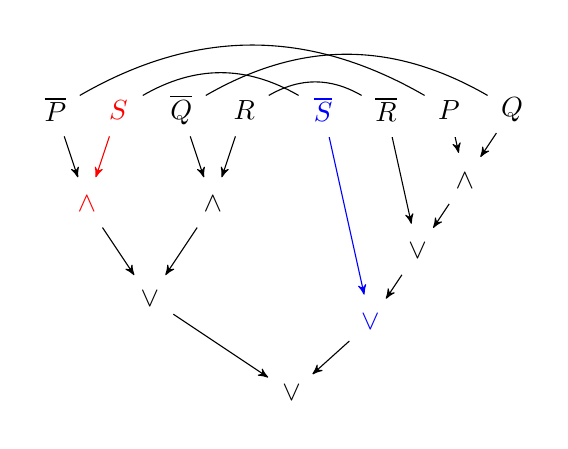
\begin{tikzpicture}
  \tikzstyle{every node}=[circle, minimum size=20pt, inner sep=2pt]
  \draw (0, 0) node (par1) {$\cor$};
  \draw (1, 0.9) node (par3) {\color{blue} $\cor$};
  \draw (-1.8, 1.2) node (par2) {$\cor$};
  \draw (-2.6, 2.4) node (tens1) {\color{red} $\cand$};
  \draw (-1, 2.4) node (tens2) {$\cand$};
  \draw (-2.2, 3.6) node (S) {\color{red} $S$};
  \draw (-0.6, 3.6) node (R) {$R$};
  \draw (-3, 3.6) node (nP) {$\overline{P}$};
  \draw (-1.4, 3.6) node (nQ) {$\overline{Q}$};
  \draw (0.4, 3.6) node (nS) {\color{blue} $\overline{S}$};
  \draw (1.6, 1.8) node (par4) {$\cor$};
  \draw (2.2, 2.7) node (tens3) {$\cand$};
  \draw (2, 3.6) node (P) {$P$};
  \draw (2.8, 3.6) node (Q) {$Q$};
  \draw (1.2, 3.6) node (nR) {$\overline{R}$};
  \draw (par2) -- (par1) [->];
  \draw (par3) -- (par1) [->];
  \draw (tens1) -- (par2) [->];
  \draw (tens2) -- (par2) [->];
  \draw (nP) -- (tens1) [->];
  \draw (S) -- (tens1) [->, color=red];
  \draw (nQ) -- (tens2) [->];
  \draw (R) -- (tens2) [->];
  \draw (nS) -- (par3) [->, color=blue];
  \draw (nR) -- (par4) [->];
  \draw (tens3) -- (par4) [->];
  \draw (P) -- (tens3) [->];
  \draw (Q) -- (tens3) [->];
  \draw (par4) -- (par3) [->];
  \draw (nP) to [bend left] (P);
  \draw (nQ) to [bend left] (Q);
  \draw (S) to [bend left] (nS);
  \draw (R) to [bend left] (nR);
\end{tikzpicture}

\caption{A unification net and its frame. The colored part shows how the
dependency ${\color{red} \exists x} \rightarrow {\color{blue} \forall z}$ is
transformed.}
\end{center}
\end{figure}

We have the following results: 

Let $u$ and $v$ be atoms or quantifiers in a unification structure $\theta$. Then they are connected by a switching path in the unification structure if, and only if, their corresponding nodes are connected by a switching path in $\theta_m$.

Consider now a switching graph $H$ of a unification structure $\theta$ of $A$.

If $H$ contains a cycle, then the corresponding switching graph of $\theta_m$
also contains a cycle. Hence, by applying the propositional results (Theorem 7)
from \cite{retore:03}, we conclude that there exists a chordless, alternating, and elementary cycle in the bicoloured graph ($W, E_W \uplus L_W$), which corresponds to an induced bimatching in the linked fograph. (Note that the linked fograph (cograph) corresponding to $\theta_m$ is equivalent to the one corresponding to $\theta$.)

\end{proof}
\end{proposition}

\subsection{From contraction/weakening to skew bifibrations}

We first introduce the atomic contraction rule, the medial rule, and two rules
on quantifiers.

\begin{center}
\begin{prooftree}
  \hypo{\vdash S\{a \cor a\}}
  \infer1[$\acD$]{\vdash S\{a\}}
\end{prooftree}
\qquad
\begin{prooftree}
  \hypo{\vdash S\{(A \cand B) \cor (C \cand D)\}}
  \infer1[$\me$]{\vdash S\{(A \cor C) \cand (B \cor D)\}}
\end{prooftree}
\\[1.5ex]
\begin{prooftree}
  \hypo{\vdash S\{\exists x A \cor \exists x B\}}
  \infer1[$\mee$]{\vdash S\{\exists x (A \cor B)\}}
\end{prooftree}	
\qquad
\begin{prooftree}
  \hypo{\vdash S\{\forall x A \cor \forall x B\}}
  \infer1[$\meee$]{\vdash S\{\forall x (A \cor B)\}}
\end{prooftree}	
\end{center}

Here, we also consider the equivalence generated by the associativity, commutativity of $\cor$ and the equations $\ttt \cor A \equiv \ttt$ and $\fff \cor A \equiv A$.

Now we have the following lemma:

\begin{lemma}
\label{lemma_ctr}
The contraction rule $\cD$ is derivable for $\{\acD, \me, \mee, \meee\}$.
\end{lemma}
\begin{proof}
	We prove that there is always $\vlderivation{\vlde{}{\{\acD, \me, \mee,
	\meee\}}{A}{\vlhy {A \cor A}}}$ by structural induction on $A$.
\begin{itemize}
  \item If $A = \ttt$ or $A = \fff$, we have 
	  \begin{prooftree} 
	    \hypo{\vdash S\{A \cor A\}}
	    \infer1[$\equiv$]{\vdash S\{A\}}
	  \end{prooftree}. (the premiss and the conclusion are equivalent)
  \item If $A = a$, then we have 
	  \begin{prooftree}
	    \hypo{\vdash S\{a \cor a\}}
	    \infer1[$\acD$]{\vdash S\{a\}}.
	  \end{prooftree}
  \item If $A = A_1 \cor A_2$, then by the induction hypothesis, we have 
	  $\vlderivation{\vlde{}{\{\acD, \me, \mee,
	\meee\}}{A_i}{\vlhy {A_i \cor A_i}}}$ for $i = 1, 2$.
	
	Hence, we have
	\begin{prooftree}
	  \hypo{\vdash S\{(A_1 \cor A_2) \cor (A_1 \cor A_2)\}}
	  \infer1[$\equiv$]{\vdash S\{(A_1 \cor A_1) \cor (A_2 \cor A_2)\}}
	  \ellipsis{$\{\acD, \me, \mee, \meee\}$}
		   {\vdash S\{A_1 \cor (A_2 \cor A_2)\}}
	  \ellipsis{$\{\acD, \me, \mee, \meee\}$}
		   {\vdash S\{A_1 \cor A_2\}}
	\end{prooftree}
  \item If $A = A_1 \cand A_2$, then by the induction hypothesis, we have 
$\vlderivation{\vlde{}{\{\acD, \me, \mee, \meee\}}{A_i}
	      {\vlhy {A_i \cor A_i}}}$ for $i = 1, 2$.

 	Hence, we have
	\begin{prooftree}
	  \hypo{\vdash S\{(A_1 \cand A_2) \cor (A_1 \cand A_2)\}}
	  \infer1[$\me$]{\vdash S\{(A_1 \cor A_1) \cand (A_2 \cor A_2)\}}
	  \ellipsis{$\{\acD, \me, \mee, \meee\}$}
		   {\vdash S\{A_1 \cand (A_2 \cor A_2)\}}
	  \ellipsis{$\{\acD, \me, \mee, \meee\}$}
		   {\vdash S\{A_1 \cand A_2\}}
	\end{prooftree}
  \item If $A = \exists x A'$, then by the induction hypothesis, we have $\vlderivation{\vlde{}{\{\acD, \me, \mee,
	\meee\}}{A'}{\vlhy {A' \cor A'}}}$.

	Hence, we have
	\begin{prooftree}
	  \hypo{\vdash S\{\exists x A' \cor \exists x A'\}}
 	  \infer1[$\mee$]{\vdash S\{\exists x (A' \cor A')\}}
	  \ellipsis{$\{\acD, \me, \mee, \meee\}$}
		   {\vdash S\{\exists x A'\}}
	\end{prooftree}
  \item If $A = \forall x A'$, then by the induction hypothesis, we have $\vlderivation{\vlde{}{\{\acD, \me, \mee,
	\meee\}}{A'}{\vlhy {A' \cor A'}}}$.

	Hence, we have
	\begin{prooftree}
	  \hypo{\vdash S\{\forall x A' \cor \forall x A'\}}
 	  \infer1[$\meee$]{\vdash S\{\forall x (A' \cor A')\}}
	  \ellipsis{$\{\acD, \me, \mee, \meee\}$}
		   {\vdash S\{\forall x A'\}}
	\end{prooftree}

\end{itemize}

\end{proof}

\begin{lemma}
The rules $\mee$ and $\meee$ are derivable for $\{\wD, \cD\}$.
\end{lemma}

\begin{proof}
We have:
\begin{center}
\begin{prooftree}
  \hypo{\vdash S\{\exists x A\}}
  \infer1[$\equiv$]{\vdash S\{\exists x (A \cor \fff)\}}
  \infer1[$\wD$]{\vdash S\{\exists x (A \cor B)\}}
\end{prooftree}
\hspace{0.5cm}
and 
\hspace{0.5cm}
\begin{prooftree}
  \hypo{\vdash S\{\exists x B\}}
  \infer1[$\equiv$]{\vdash S\{\exists x (\fff \cor B)\}}
  \infer1[$\wD$]{\vdash S\{\exists x (A \cor B)\}}
\end{prooftree}
\end{center}
Thus, we have:

\begin{center}
\begin{prooftree}
  \hypo{\vdash S\{\exists x A \cor \exists x B\}}
  \ellipsis{}{\vdash S\{\exists x (A \cor B) \cor \exists x (A \cor B)\}}
  \infer1[$\cD$]{\vdash S\{\exists x (A \cor B)\}}
\end{prooftree}
\end{center}
Similar for $\meee$.
\end{proof}

Now we define a propositional encoding for first-order formulas.

\begin{definition}
The propositional encoding $\PE{A}$ of a formula $A$ is defined inductively by:

\begin{centering}
	$\PE{a} = a$ for every atom $a$

	$\PE{(A \cor B)} = \PE{A} \cor \PE{B}$ \hspace{2cm} $\PE{(A \cand B)} =
	\PE{A} \cand \PE{B}$

	$\PE{(\forall x A)} = U_x \cor \PE{A}$ \hspace{2cm} $\PE{(\exists x A)}
	= E_x \cand \PE{A}$

\end{centering}
where $U_x$ and $E_x$ are fresh nullary atoms.

\end{definition}

Similarly, we can define the propositional encoding $\PE{S}$ of a context $S$
inductively by setting $\PE{\Box} = \Box$. Note that $\PE{S}$ is also a context.

We have the following facts:

\begin{proposition}
For any context $S$ and any formula $A$:
\begin{itemize}
  \item $\PE{A}$ is a formula containing no quantifier for any formula $A$.
  \item $\graphof(\PE{A}) = \graphof(A)$ by confounding the atoms $U_x$, $E_x$ with the variable
	  $x$. Thus, a map $f : \graphof(\PE{A}) \rightarrow \graphof(\PE{B})$ can be seen as a map
		$f : \graphof(A) \rightarrow \graphof(B)$.
  \item $\PE{(S\{A\})} = \PE{S}\{\PE{A}\}$.
\end{itemize}

\end{proposition}

\begin{proposition}
\label{prop311}
Let $A$ and $B$ be two formulas such that
$\od{\odd{\odh {A}}{}{B}{\{\wD, \cD\}}}$. Then 
$\od{\odd{\odh {\PE{A}}}{}{\PE{B}}{\{\wD, \cD\}}}$.
\end{proposition}
\begin{proof}
  Trivial by induction.
\end{proof}

\begin{lemma}
\label{mlem}
	Given two formulas $A$ and $B$ and a derivation $\od{\odd{\odh {A}}
	{\Delta}{B}{\{\wD, \cD\}}}$, then there exists a skew bifibration $G(A)
	\rightarrow G(B)$.
\end{lemma}

\begin{proof}
By Lemma \ref{lemma_ctr}, there exists a derivation $\od{\odd{\odh {A}}
	{\Delta}{B}{\{\wD, \acD, \me, \mee, \meee \}}}$.
	
For each rule from $\{\wD, \acD, \me, \mee, \meee \}$, we define a map and show that it is a skew fibration.

\begin{itemize}
  \item \begin{prooftree}
  \hypo{\vdash S\{\fff \}}
  \infer1[$\wD$]{\vdash S\{A\}}
\end{prooftree}:

  the map $wk$ maps $\fff$ to anything and is identity elsewhere.   
 
  \item
    \begin{prooftree}
      \hypo{\vdash S\{a \cor a\}}
       \infer1[$\acD$]{\vdash S\{a\}} 
    \end{prooftree}: 
    
    the map $ac$ maps the two $a$-labelled literals in the premise to the $a$-labelled literal in the conclusion.

  \item 
    \begin{prooftree}
      \hypo{\vdash S\{(A \cand B) \cor (C \cand D)\}}
      \infer1[$\me$]{\vdash S\{(A \cor C) \cand (B \cor D)\}}
    \end{prooftree}:
    
    the map $m$ is the canonical identity that maps $A$ to $A$, $\cdots$, $D$ to $D$.
  \item 
    \begin{prooftree}
      \hypo{\vdash S\{\exists x A \cor \exists x B\}}
      \infer1[$\mee$]{\vdash S\{\exists x (A \cor B)\}}
    \end{prooftree}: 
   
    the map $m_1$ maps the two $x$-labelled binders in the premise to the $x$-labelled binder in the conclusion,  $A$ to $A$ and $B$ to $B$.
  \item
    \begin{prooftree}
      \hypo{\vdash S\{\forall x A \cor \forall x B\}}
      \infer1[$\meee$]{\vdash S\{\forall x (A \cor B)\}}
    \end{prooftree}:
    
    the map $m_2$ maps the two $x$-labelled binders in the premise to the $x$-labelled binder in the conclusion,  $A$ to $A$ and $B$ to $B$. 

\end{itemize}

By considering propositional encodings, the maps defined are label-preserving
skew fibrations on the underlying fographs according to
\cite{str:07:RTA}.

Now we prove that each map $g \in \{wk, ac, m, m_1, m_2 \}$ is a skew bifibration. To do that, it suffices to prove that $g$ is a fibration between the corresponding binding graphs since it is already a skew fibration on the corresponding fographs and it is label-preserving and existential-preserving.
\begin{center}
for each $x$-binder $b$ in $\graphof(\PE{B})$, for each vertex $v \in V(\graphof(\PE{A}))$
such that $g(v)$ is bound by $b$, there exists a unique binder $b'$ such
that $b'$ binds $v$.
\end{center}

\begin{itemize}
  \item $wk$ and $m$ are clearly fibrations: the binding relations of the premise and the conclusion are exactly the same.
  \item $ac$ is a fibration: suppose that $a$ that in the conclusion $a$ is bound by some quantifier $b$ in $S$, then for each of its preimages by $ac$, there exists exactly one binder (in fact, $b$) in $S$ that binds it.
  \item $m_1$ and $m_2$ are fibrations: in the conclusion, for every atom $a$ in $A \cor B$ bound by the $x$-labelled quantifier, $a$ has exactly one preimage and it is bound by the $x$-llabelled quantifier in the premise.
\end{itemize}

  Therefore, all of these maps are skew bifibrations and since skew bifibrations
on fographs compose (Lemma 10.32, \cite{hughes:fopws}), there exists a skew
bifibration from $\graphof(A)$ to $\graphof(B)$.

\end{proof}

\begin{theorem_}
If a formula $A$ is provable in $\LK$, then it has a combinatorial proof.
\end{theorem_}

\begin{proof}
By Theorem \ref{thm1}, there exists a formula $A'$ such that there is a proof
$\Pi$ of $A'$ in $\FOMLL$ and a derivation $D$ from $A'$ to $A$ consisting of
the $\wD$ and $\cD$ rules only. The proof $\Pi$ corresponds to a unique
unification net which is equivalent to the fonet corresponding to $\Pi$, i.e.,
the fograph $\graphof(A')$ together with the links of $\Pi$. By Lemma \ref{mlem}, 
there exists a skew bifibration $\graphof(A') \rightarrow \graphof(A)$. We have thus a
combinatorial proof of $A$.

\end{proof}

\subsection{From skew bifibrations to contraction/weakening}

\begin{theorem_}
Let $A$ and $B$ be two formulas and $f: G(A) \rightarrow G(B)$ a skew bifibration. Then there exists a derivation $\od{\odd{\odh {A}}{\Delta}{B}{\{\wD, \cD\}}}$.
\end{theorem_}

$f$ can be seen as a skew fibration from $G(\PE{A})$ to $G(\PE{B})$, which gives the existence of the propositions $A'$ and $B'$, and of the following derivation:
  \[\od{\odd{\odd{\odd{\odh{\PE{A}} }
  {\Delta }{A'}{\me} }
  {\Delta' }{B'}{\acD} }
  {\Delta''}{\PE{B}}{\wD}} \]

\begin{lemma} there exists $B''$ such that $\PE{B''}$ = $B'$.

\begin{proof}
Consider the dervation $\Delta''$. If some $U_x$ (or $E_x$) is introduced
via weakening, then all the atoms it binds in $\PE{B}$ should also be introduced 
via weakening. In fact, an atom of $\PE{B}$ is introduced via weakening is 
equivalent to the fact that its corresponding vertex is not in the image of $f$. 
Since there is an edge from $U_x$ (resp. $E_x$) to all the literals it binds in the 
binding graph $\overrightarrow{\graphof(B)}$, if one of the atoms is in the image, 
$U_x$ (resp. $E_x$) should also be in the image since $f$ is a fibration on binding graphs.

This means that a such $B''$ can be obtained from $B$ by erasing all the $U_x$ and $E_x$ introduced via weakening and all the atoms they bind.
\end{proof}
\end{lemma}

We introduce new (atomic) symbols $E_x^*$ and $U_x^*$ which are used to
represent disjunctions of $E_x$ and $U_x$ respectiveley.

We define a translation $(\cdot)^*$ inductively by:
\begin{itemize}
  \item $(E_x \cor \cdots \cor E_x)^* = E_x$
  \item $(U_x \cor \cdots \cor U_x)^* = U_x$
  \item structural recursion in all the other cases.
\end{itemize}

Then the derivation:
 \[\od{\odd{\odd{\odh{\PE{A}} }
  {\Delta }{A'}{\me} }
  {\Delta' }{\PE{B''}}{\acD}} \]
can be translated to the derivation:
\[\od{\odd{\odh{(\PE{A})^*} }
{\Delta^* }{(\PE{B''})^*}{}} \]

where $\Delta^*$ is the derivation obtained by replacing all the formulas $F$
with $F^*$ and by applying the following rule transformation:

\begin{center}
\mbox{
\begin{prooftree}
  \hypo{S\{Q_x\}}
  \infer1[$\acD$]{S\{Q_x\}}
\end{prooftree}

$\leadsto$

\begin{prooftree}
  \hypo{S\{Q_x\}}
  \infer1[$=$]{S\{Q_x\}}
\end{prooftree}

}
\vspace{0.4cm}

\mbox{
\begin{prooftree}
  \hypo{S\{(E_x \cand C) \cor (E_x \cand D)\}}
  \infer1[$\me$]{S\{E_x \cand (C \cor D)\}}
\end{prooftree}

$\leadsto$

\begin{prooftree}
  \hypo{S\{(E_x \cand C) \cor (E_x \cand D)\}}
  \infer1[$\me'$]{S\{E_x \cand (C \cor D)\}}
\end{prooftree}

}
	
\end{center}
where $Q_x$ stands for $E_x$ or $U_x$.

$\Delta^*$ can now be transformed into a valid derivation $\Delta_1$ by using the two
transformation rules above and by applying them in a bottom-up style:
\[\od{\odd{\odh{(\PE{A})^*} }
{\Delta_1 }{(\PE{B''})^*}{\acD, \me, \me'}} \]

\begin{lemma}
Every line of $\Delta_1$ is a propositional encoding.

\begin{proof}
We proceed by bottom-up induction in the derivation.
Clearly, $(\PE{B''})^*$ is a propositional encoding as there is no disjunction of $Q_x$
in it.

First consider the $\acD$ rule:
\begin{prooftree}
  \hypo{C \cor C}
  \infer1[$\acD$]{C}
\end{prooftree}

It is clear that if $C$ is a propositional encoding, then so is $C \cor C$.

Now consider the $\me$ rule:
\begin{center}
\begin{prooftree}
  \hypo{S\{(C \cand D) \cor (E \cand F)\}}
  \infer1[$\me$]{S\{(C \cor E) \cand (D \cor F)\}}
\end{prooftree}
\end{center}
Suppose that $(C \cor E) \cand (D \cor F) = \PE{G}$ for some $G$.
Since $C \cor E$ cannot be $Q_x$ (otherwise, the rule applied would be
$\me'$), $G$ can be written as $G_1 \cand G_2$ with $C \cor E = \PE{G_1}$ and $D
\cor F = \PE{G_2}$.

We have thus $G_i = \forall x_i H_i$ or $J_i \cor K_i (i = 1, 2)$.

If $G_i = \forall x H_i$ for some $i$, then there will be a conjunction of $U_x$
and some formula which can never be eliminated by the rules $\me$, $\me'$ and
$\acD$. However, there exists no such conjunction in ${\PE{A}}^*$, which leads to a
contradiction.

Hence, $G_i$ can be written as $J_i \cor K_i$ for $i = 1, 2$. We now have $(C
\cand D) \cor (E \cand F) = \PE{((J_1 \cand J_2) \cor (K_1 \cand
K_2))}$.

Finally, consider the $\me'$ rule:
\begin{center}
\begin{prooftree}
  \hypo{S\{(E_x \cand C) \cor (E_x \cand D)\}}
  \infer1[$\me'$]{S\{E_x \cand (C \cor D)\}}
\end{prooftree}
\end{center}
Suppose that $E_X \cand (C \cor D)$ = $\PE{F}$ for some $F$. It is clear
that $F = \exists x G$ with $\PE{G} = C \cor D$ for some $G$.
We distinguish two cases:
\begin{itemize}
  \item $G = \forall y H$: in this case, $(E_x \cand C) \cor (E_x \cand
D)$ has a subformula $(E_x \cand U_y)$, which cannot be eliminated by the
	rules $\me$, $\me'$, $\acD$. It is clear that ${\PE{A}}^*$ does not
have a subformula of this form, which leads to a contradiction.
  \item $G = G_1 \cor G_2$: in this case, $(E_x \cand C) \cor (E_x \cand
  D) = \PE{((\exists x G_1) \cor (\exists x G_2))}$.
\end{itemize}

\end{proof}	
\end{lemma}


\hrule
    \begin{itemize}
    \item If none of
    the four principal formulas in the premise is $x$ or $x\vlor F$ or
    $x\vlan F$ for some formula $F$ and $x\in\VAR$, then this instance
    of $\me$ can trivially be lifted, and and we can proceed by
    induction hypothesis.
  \item If exactly one of the four principal formulas in the premise
    is $x$ for some $x\in\VAR$, then this $x$ is the encoding of an existential in the
    premise and of an universal in the conclusion. This is impossible,
    as $\phi$ has to preserve existentials.
  \item If two of the four principal formulas in the premise
    are $x$ for some $x\in\VAR$, then we are in the following special case of~\eqref{eq:mac}:
      \begin{equation*}
        \vlderivation{
          \vlin{\acDeq}{}{\Scons{x\vlan(C\vlor D)}}{
            \vlin{\me}{}{\Scons{(x\vlor x)\vlan(C\vlor D)}}{
              \vlhy{\Scons{(x\vlan C)\vlor (x\vlan D)}}}}}
      \end{equation*}
      which can be lifted immediately to
      \begin{equation*}
        \vlinf{\mexD}{}{\Scons{\exists x.(C\vlor D)}}{\Scons{(\exists x.C)\vlor(\exists x.D)}}
      \end{equation*}



  \item $\me/\acDx$ as in situation~\eqref{eq:mac}: We must have
    $R_1\cons{x}\fequ x\vlor E$ for some $E$ and $R_2\cons{x}\fequ
    x\vlor F$ for some $F$ with $R\cons{x}\fequ x\vlor E\vlor
    F$. Otherwise, the application of $\acDeq$ would not be correct.
    We have the following four cases: 
%    \begin{itemize}
    \item $E$ and $F$ are both non-empty: Then~\eqref{eq:mac} is (modulo
      omitted applications of $\fequ$):
      \begin{equation*}
        \vlderivation{
          \vlin{\acDeq}{}{\Scons{(x\vlor E\vlor F)\vlan(C\vlor D)}}{
            \vlin{\me}{}{\Scons{((x\vlor E)\vlor (x\vlor F))\vlan(C\vlor D)}}{
              \vlhy{\Scons{((x\vlor E)\vlan C)\vlor ((x\vlor F)\vlan D)}}}}}
      \end{equation*}
      which can be lifted to
      \begin{equation*}
        \vlderivation{
          \vlin{\mfaD}{}{\Scons{(\forall x.(E\vlor F))\vlan(C\vlor D)}}{
            \vlin{\me}{}{\Scons{((\forall x. E)\vlor (\forall x. F))\vlan(C\vlor D)}}{
              \vlhy{\Scons{((\forall x. E)\vlan C)\vlor ((\forall x. F)\vlan D)}}}}}
      \end{equation*}
    \juihsuan{maybe need some words to exclude the case in which $C$ (or $D$)
is a propositional variable.}\lutz{shit. (you mean a ``first order variable'') this actually can happen. then we have another $\mexD$}
    \item $E$ is empty and $F$ is not: Then~\eqref{eq:mac} becomes
      \begin{equation*}
        \vlderivation{
          \vlin{\acDeq}{}{\Scons{(x\vlor F)\vlan(C\vlor D)}}{
            \vlin{\me}{}{\Scons{(x\vlor (x\vlor F))\vlan(C\vlor D)}}{
          \vlhy{\Scons{(x\vlan C)\vlor ((x\vlor F)\vlan D)}}}}}
      \end{equation*}
      The conclusion is the propositional encoding of $\Scons{(\forall
        x. F)\vlan(C\vlor D)}$ and the premise is the propositional
      encoding of $\Scons{(\exists x.C)\vlor ((\forall x. F)\vlor
        D)}$. Also note that no $\me$-instance can break up the
      conjunction in $x\vlan C$ in the premise. Hence, $\phi$ maps an
      existential to a universal, which is ruled out by the
      definition. Hence, this case cannot occur.
    \item $E$ is non-empty and $F$ is empty: This case is similar to the
      previous subcase.
    \item   $E$ and $F$ are both empty: Then~\eqref{eq:mac} is
      \begin{equation*}
        \vlderivation{
          \vlin{\acDeq}{}{\Scons{x\vlan(C\vlor D)}}{
            \vlin{\me}{}{\Scons{(x\vlor x)\vlan(C\vlor D)}}{
              \vlhy{\Scons{(x\vlan C)\vlor (x\vlan D)}}}}}
      \end{equation*}
      which can be lifted immediately to
      \begin{equation*}
        \vlinf{\mexD}{}{\Scons{\exists x.(C\vlor D)}}{\Scons{(\exists x.C)\vlor(\exists x.D)}}
      \end{equation*}
    \end{itemize}



% An example of a floating figure using the graphicx package.
% Note that \label must occur AFTER (or within) \caption.
% For figures, \caption should occur after the \includegraphics.
% Note that IEEEtran v1.7 and later has special internal code that
% is designed to preserve the operation of \label within \caption
% even when the captionsoff option is in effect. However, because
% of issues like this, it may be the safest practice to put all your
% \label just after \caption rather than within \caption{}.
%
% Reminder: the "draftcls" or "draftclsnofoot", not "draft", class
% option should be used if it is desired that the figures are to be
% displayed while in draft mode.
%
%\begin{figure}[!t]
%\centering
%\includegraphics[width=2.5in]{myfigure}
% where an .eps filename suffix will be assumed under latex, 
% and a .pdf suffix will be assumed for pdflatex; or what has been declared
% via \DeclareGraphicsExtensions.
%\caption{Simulation results for the network.}
%\label{fig_sim}
%\end{figure}

% Note that the IEEE typically puts floats only at the top, even when this
% results in a large percentage of a column being occupied by floats.


% An example of a double column floating figure using two subfigures.
% (The subfig.sty package must be loaded for this to work.)
% The subfigure \label commands are set within each subfloat command,
% and the \label for the overall figure must come after \caption.
% \hfil is used as a separator to get equal spacing.
% Watch out that the combined width of all the subfigures on a 
% line do not exceed the text width or a line break will occur.
%
%\begin{figure*}[!t]
%\centering
%\subfloat[Case I]{\includegraphics[width=2.5in]{box}%
%\label{fig_first_case}}
%\hfil
%\subfloat[Case II]{\includegraphics[width=2.5in]{box}%
%\label{fig_second_case}}
%\caption{Simulation results for the network.}
%\label{fig_sim}
%\end{figure*}
%
% Note that often IEEE papers with subfigures do not employ subfigure
% captions (using the optional argument to \subfloat[]), but instead will
% reference/describe all of them (a), (b), etc., within the main caption.
% Be aware that for subfig.sty to generate the (a), (b), etc., subfigure
% labels, the optional argument to \subfloat must be present. If a
% subcaption is not desired, just leave its contents blank,
% e.g., \subfloat[].


% An example of a floating table. Note that, for IEEE style tables, the
% \caption command should come BEFORE the table and, given that table
% captions serve much like titles, are usually capitalized except for words
% such as a, an, and, as, at, but, by, for, in, nor, of, on, or, the, to
% and up, which are usually not capitalized unless they are the first or
% last word of the caption. Table text will default to \footnotesize as
% the IEEE normally uses this smaller font for tables.
% The \label must come after \caption as always.
%
%\begin{table}[!t]
%% increase table row spacing, adjust to taste
%\renewcommand{\arraystretch}{1.3}
% if using array.sty, it might be a good idea to tweak the value of
% \extrarowheight as needed to properly center the text within the cells
%\caption{An Example of a Table}
%\label{table_example}
%\centering
%% Some packages, such as MDW tools, offer better commands for making tables
%% than the plain LaTeX2e tabular which is used here.
%\begin{tabular}{|c||c|}
%\hline
%One & Two\\
%\hline
%Three & Four\\
%\hline
%\end{tabular}
%\end{table}


% Note that the IEEE does not put floats in the very first column
% - or typically anywhere on the first page for that matter. Also,
% in-text middle ("here") positioning is typically not used, but it
% is allowed and encouraged for Computer Society conferences (but
% not Computer Society journals). Most IEEE journals/conferences use
% top floats exclusively. 
% Note that, LaTeX2e, unlike IEEE journals/conferences, places
% footnotes above bottom floats. This can be corrected via the
% \fnbelowfloat command of the stfloats package.



\end{document}
